%\begin{sidewaysfigure}
%  \begin{center}
%  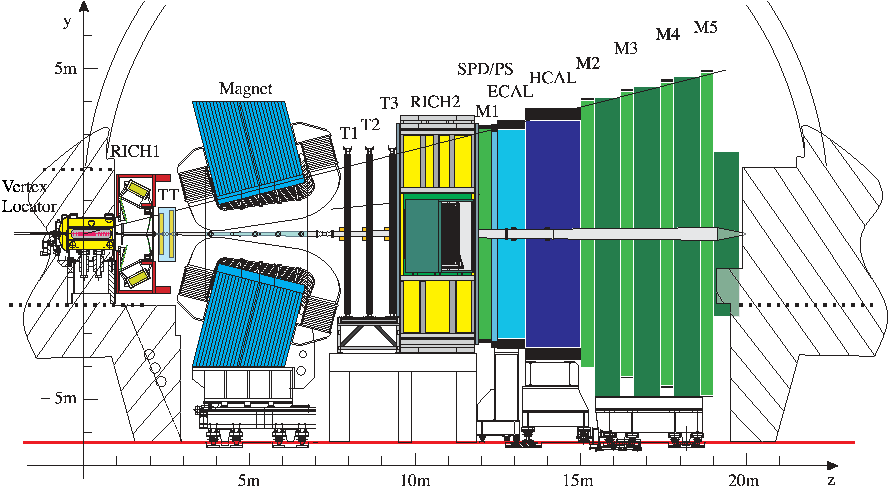
\includegraphics[width=0.8\textheight]{lhcb-detector-cross-section}
%  \caption[Cross-section view of \LHCb, cut in the non-bending $y$--$z$ plane]%
%    {Cross-section view of \LHCb, cut in the non-bending $y$--$z$ plane.}
%  \label{fig:LHCbCrossSection}
%  \end{center}
%\end{sidewaysfigure}



\chapter{Measurement of the $\nu_\mu$ charged current inclusive cross-section on Pb}
\label{chap:CrossSectionMeasurement}
This chapter presents the measurement of the $\nu_\mu$ CC inclusive cross-section on Pb using the ND280 ECals.  This chapter details the measurement method, the samples used in the measurement, the assessment of the systematic uncertainties, validation of the measurement method and finally the measurement itself.

\section{Measurement method}
\label{sec:MeasurementMethod}
The chosen method fits a prediction to measured data using multiple data samples~\cite{PhysRevD.78.032003, PhysRevD.83.012005}\Yoshi{}{ADDRESSED - I put the references at the end of the sentence because the text doesn't flow well if the first sentence in the chapter is cut off after just ``The chosen method''.}.  \Yoshi{Here, a ``sample'' refers to, for example, selected events in a particular ECal module.}{ADDRESSED - because ``sample could mean anything (e.g., different run periods or something), and without some idea of what it refers to, it is hard to follow the rest.} The core of the analysis method is a $\chi^2$ fit which tries to minimise the difference between the prediction and the data.  The $\chi^2$ is defined as 
\begin{equation}
  \chi^2 = \Delta \vec{N}^{\textrm{T}} \left(\underline{\underline{V}}^{\textrm{syst}} + \underline{\underline{V}}^{\textrm{stat}} \right)^{-1} \Delta \vec{N},
  \label{eqn:Chi2Def}
\end{equation}
where $\underline{\underline{V}}^{\textrm{syst}}$ and $\underline{\underline{V}}^{\textrm{stat}}$ are the systematic and statistical covariance matrices for the sample and $\Delta\vec{N}$ contains the difference between the data and the prediction for each sample.  If the number of samples used is $M$, $\Delta\vec{N}$ is defined as 
\begin{equation}
  \Delta\vec{N} = 
  \begin{pmatrix}
    N^{\textrm{data}}_1 - N^{\textrm{pred}}_1 \\
    \vdots \\
    N^{\textrm{data}}_M - N^{\textrm{pred}}_M
  \end{pmatrix}.
  \label{eqn:VecNDef}
\end{equation}
For sample $j$ of the sample set $M$, $N^{\textrm{data}}_j$ and $N^{\textrm{pred}}_j$ are the number of measured data events and number of predicted events.  The extractable information from the fit is located in $N^{\textrm{pred}}_j$ which can be subdivided into a set of templates, each of which are assigned a normalisation parameter, namely
\begin{equation}
  N^{\textrm{pred}}_j = \sum_j R_{i}n_{ij},
  \label{eqn:NPredDef}
\end{equation}
where $n_{ij}$ is the number of events in template $i$ of sample $j$ and $R_{i}$ is the normalisation assigned to that template.  The normalisation parameters are free to float in the fit and so it  is in the normalisation parameters that the desired physical information is located.
\section{Input samples to the fit}
\label{sec:InputSamples}
The DS ECal provides the main signal sample which will be used to extract the cross-section.  As shown in table~\ref{table:FinalEffPur}, the selected sample in the DS ECal has the highest purity and efficiency in the whole selection making the sample the natural choice to extract the cross-section.
\newline
\newline
The method outlined above allows for the simultaneous constraint of physical parameters and the background contamination of a set of input samples.  The method works particularly well when the input samples do not share the same sensitivity to a particular background type.  For example, in ND280, each ECal module is exposed to a different beam intensity and energy spectrum and so is exposed to a unique amount of \Yoshi{beam-induced}{ADDRESSED - was beam induced. But this is a compound adjective} background.  Each ECal module can be thought of as a separate input sample which fits well with the method outlined above.  So, while the DS ECal will provide the target in which the cross-section will be extracted, the barrel ECals are to also be included in the fit as a background constraint.  To further allow the barrel ECals to achieve this, an additional sample set of barrel ECal events are to be included.  This additional sample set, called the 'reverse' sample set,  comes from the same data set as the selected sample described in chapter~\ref{chap:NeutrinoInteractionSelection}.  However, the events in the reverse sample set are events which pass the fiducial volume cuts but fail any other cut.  An example of a selected sample compared with a reverse sample is shown in Fig.~\ref{fig:NuEnergyReactionCodeBottomLeft}.  There are clear differences in the shape of the energy spectrum between Fig.~\ref{fig:NuEnergyReactionCodeBottomLeftSignal} and Fig.~\ref{fig:NuEnergyReactionCodeBottomLeftReverse}\Yoshi{,}{ADDRESSED - comma} which suggests that the selection is biased towards \Yoshi{lower-energy}{ADDRESSED - was lower energy; a compound adjective} neutrino interactions, despite the flat efficiency curves shown in Fig.~\ref{fig:EffPurSummedTopologiesBarrel}. The apparent bias is actually an effect of higher\Yoshi{-}{ADDRESSED - }energy interactions creating a surplus of reconstructed objects, most of which are cut away by the selection.  The shape of the true neutrino energy spectrum (see Fig.~\ref{fig:NSignalEventsTruthNeutrinoEnergy} for an example) is actually more like the selected sample shown in Fig.~\ref{fig:NuEnergyReactionCodeBottomLeftSignal}.
\begin{figure}%
  \centering
  \subfloat[Selected sample.]{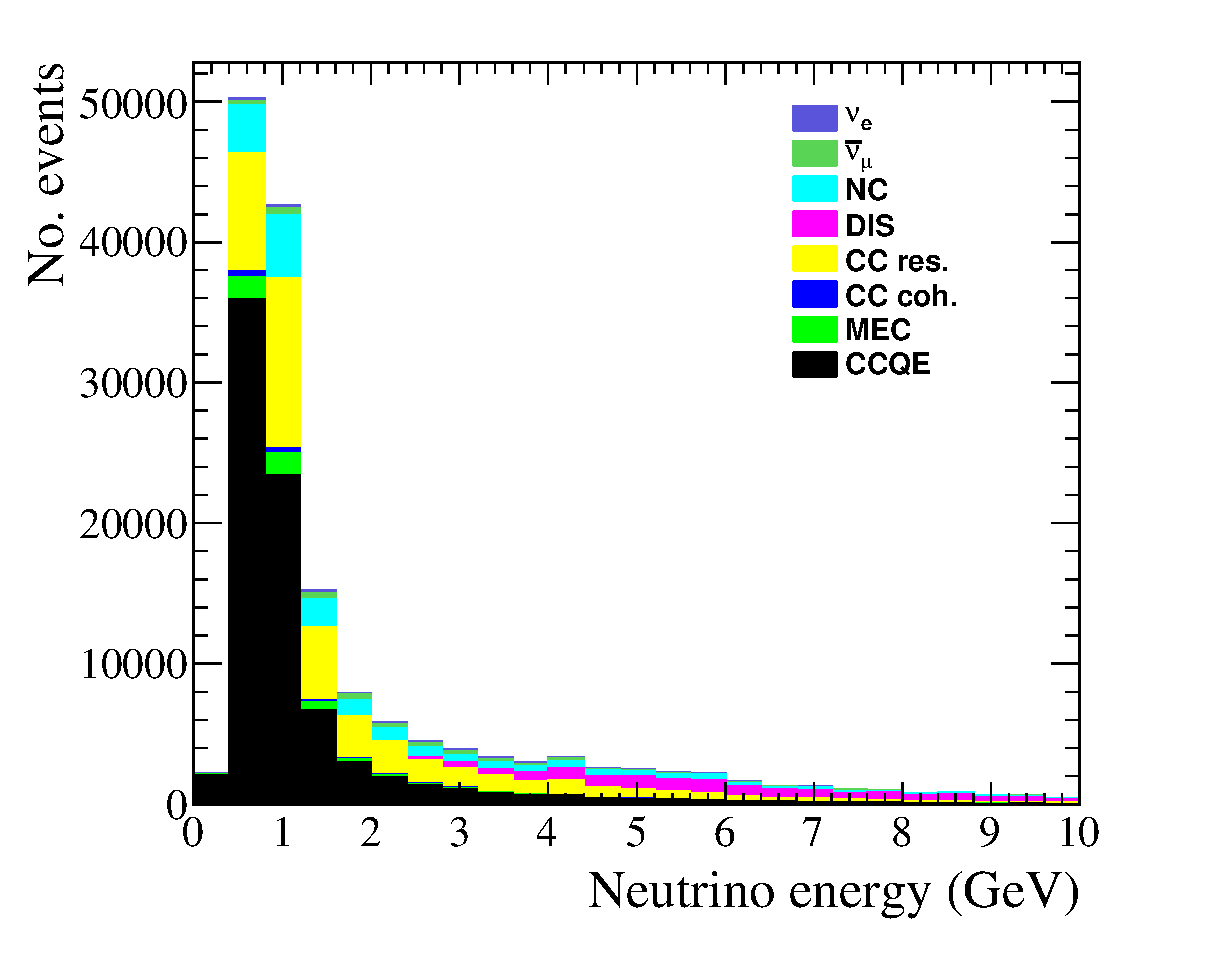
\includegraphics[width=8cm]{images/measurement/samples/NuEnergy_ReactionCode_BottomLeft_Signal.eps} \label{fig:NuEnergyReactionCodeBottomLeftSignal}}
  \subfloat[Reverse sample.]{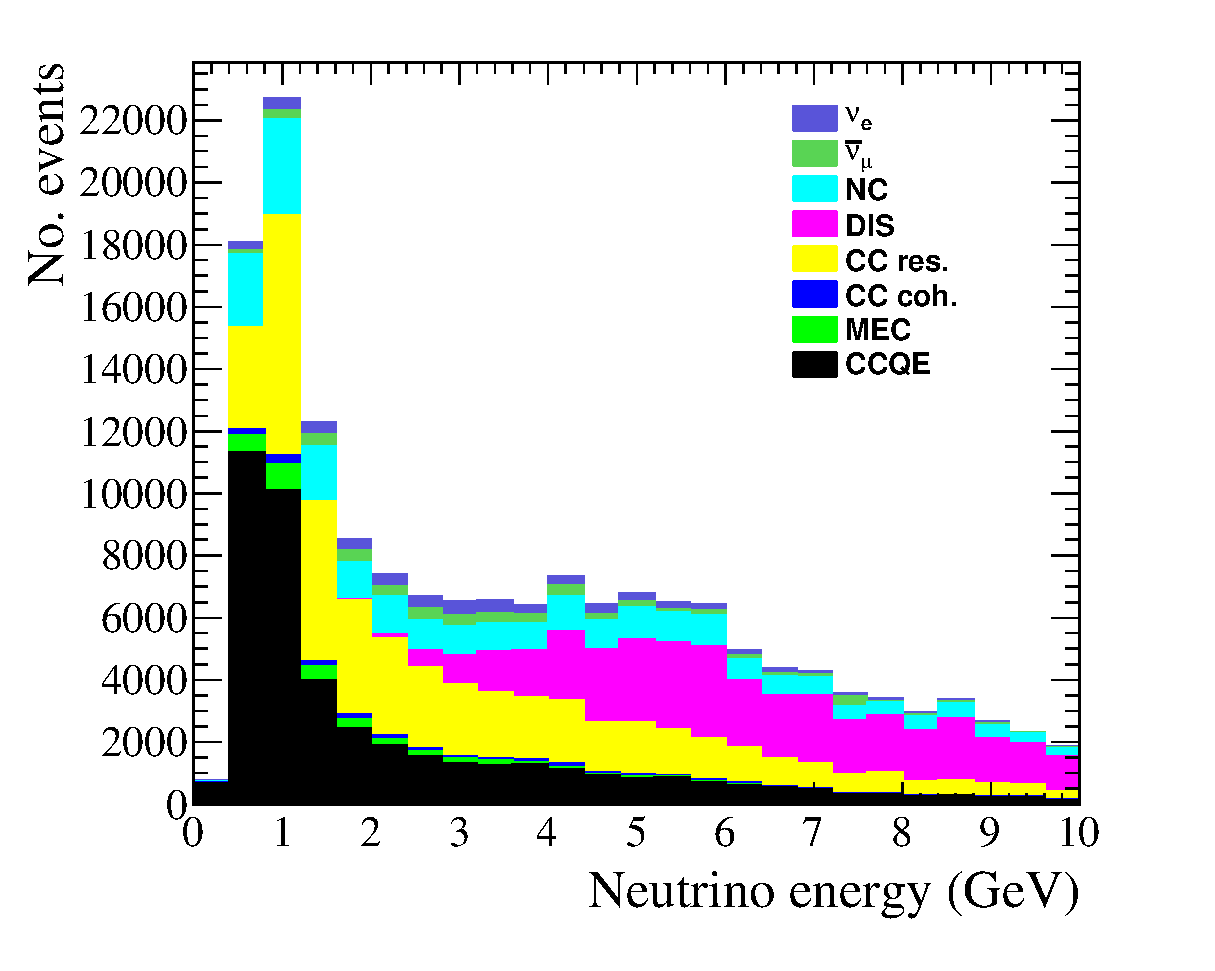
\includegraphics[width=8cm]{images/measurement/samples/NuEnergy_ReactionCode_BottomLeft_Reverse.eps} \label{fig:NuEnergyReactionCodeBottomLeftReverse}}
  \caption{The neutrino energy of events seen in the bottom-left ECal module broken down by the neutrino interaction mode. \Yoshi{The plots correspond to $3.949\times 10^{20}$~POT of simulated data.}{ADDRESSED - } \Yoshi{}{It would be nice to see the plots also with some sort of proxy for the energy as the horizontal axis---such as the total charge, or number of prongs etc. It would help the reader see what is going on.}}
  \label{fig:NuEnergyReactionCodeBottomLeft}
\end{figure}
\newline
\newline
As described in chapter~\ref{chap:NeutrinoInteractionSelection}, the developed selection does not distinguish between lead and carbon interactions, partly because such events are indistinguishable from one another.  It is\Yoshi{, however,}{ADDRESSED - } desirable to separate the two categories out\Yoshi{,}{ADDRESSED - comma} as the presented measurement purely involves lead.  As the ECal is not capable of simultaneously constraining the lead and carbon events by itself, an additional constraint is needed.  \Yoshi{Therefore}{ADDRESSED - was So}, a sample of CC interactions on carbon occurring in the FGD are also included, which are taken from the official ND280 oscillation input analysis~\cite{CCIncSelFGDTN}.
\newline
\newline
To summarise, there are many inputs samples to the measurement.  Specifically, there are \Yoshi{12 barrel ECal samples (6 selected and 6 reverse), the DS ECal sample and the FGD sample which totals to 14 input samples}{ADDRESSED - This adds up to 14 doesn't it?}.\Yoshi{}{ADDRESSED - I would also state the rough number of data and MC stats you expect in each sample---otherwise the ``samples'' sound very abstract. Something like ``The smallest sample among the ECALs is expected to contain approximately FIXME,000 real data events.''}.  To give a rough handle on the level of statistics, the DS-ECal sample, which will provide the primary interaction target events, is expected to contain 35000~events 
\newline
\newline
\Yoshi{Monte Carlo-simulated data of $3.949\times 10^{20}$~POT worth of NEUT events, which corresponds to 3 times the real data used}
{ADDRESSED - was ``In terms of statistics, $3.949\times 10^{20}$~POT worth of NEUT MC events'', but this seems a bit colloquial} are used for this measurement.
\Yoshi{}{ADDRESSED - You may also want to put this at the beginning of the section, if all plots use this amount of MC stats.}

\section{The ECal rate fit}
\label{sec:ECalRateFit}
Now that the general method and the input samples have been introduced, the fit used by the analysis can be introduced.  The fit itself is a data-driven constraint of the event rate in each ECal module where the Monte Carlo prediction is separated into templates whose normalisation is allowed to vary.  The machinery outlined in section~\ref{sec:MeasurementMethod} almost completely describes what is required to understand the fit\Yoshi{;}{ADDRESSED - was ``,''; see \url{http://www.nationalpunctuationday.com/semicolon.html}} however\Yoshi{,}{ADDRESSED - ditto} two specific definitions are needed.  The first is that there are 12 input samples to the fit.  The second is the definition of $N^{\textrm{pred}}_i$.  To constrain the lead event rate, three Monte Carlo templates are needed: a lead template which contains any reconstructed event associated with a $\nu_\mu$ CC interaction on lead\Yoshi{;}{ADDRESSED - was ``,'' but the list is set off with a colon, so a semi-colon is appropriate} a carbon template which contains any reconstructed event associated with a $\nu_\mu$ CC interaction on carbon\Yoshi{;}{ADDRESSED - ditto} and an 'other' template which contains any reconstructed event which does not fall into the above two categories.  \Yoshi{The number of predicted events in each sample $i$, }{ADDRESSED - Because you need to say somewhere what ``pred'' stands for}$N^{\textrm{pred}}_i$ is then defined as 
\begin{equation}
  N^{\textrm{pred}}_i = R^{\textrm{Pb}}n^{\textrm{Pb}}_i + R^{\textrm{C}}n^{\textrm{C}}_i + R^{\textrm{other}}n^{\textrm{other}}_i,
  \label{eqn:ECalFitPredDef}
\end{equation}
where $n^{\textrm{X}}_i$ is the number of events in template X of sample $i$ and $R^{\textrm{X}}_i$ is the variable normalisation of that template.
\newline
\newline
The rate fit allows $R^{\textrm{Pb}}_i$, $R^{\textrm{C}}_i$ and $R^{\textrm{other}}_i$ to vary with no prior constraint in an attempt to minimise the $\chi^{2}$ as defined in equation~\ref{eqn:Chi2Def}.  Once the minimum has been found, the fitted $R^{\textrm{Pb}}_i$ can then be used to extract the cross-section using the selected events in the DS ECal.  
\newline
\newline
The number of events in each input sample, broken down by the template contributions, is shown in Fig.~\ref{fig:NominalMCTemplates}.  As should be expected, the relative background contribution varies between each ECal module.
\begin{figure}
  \centering
  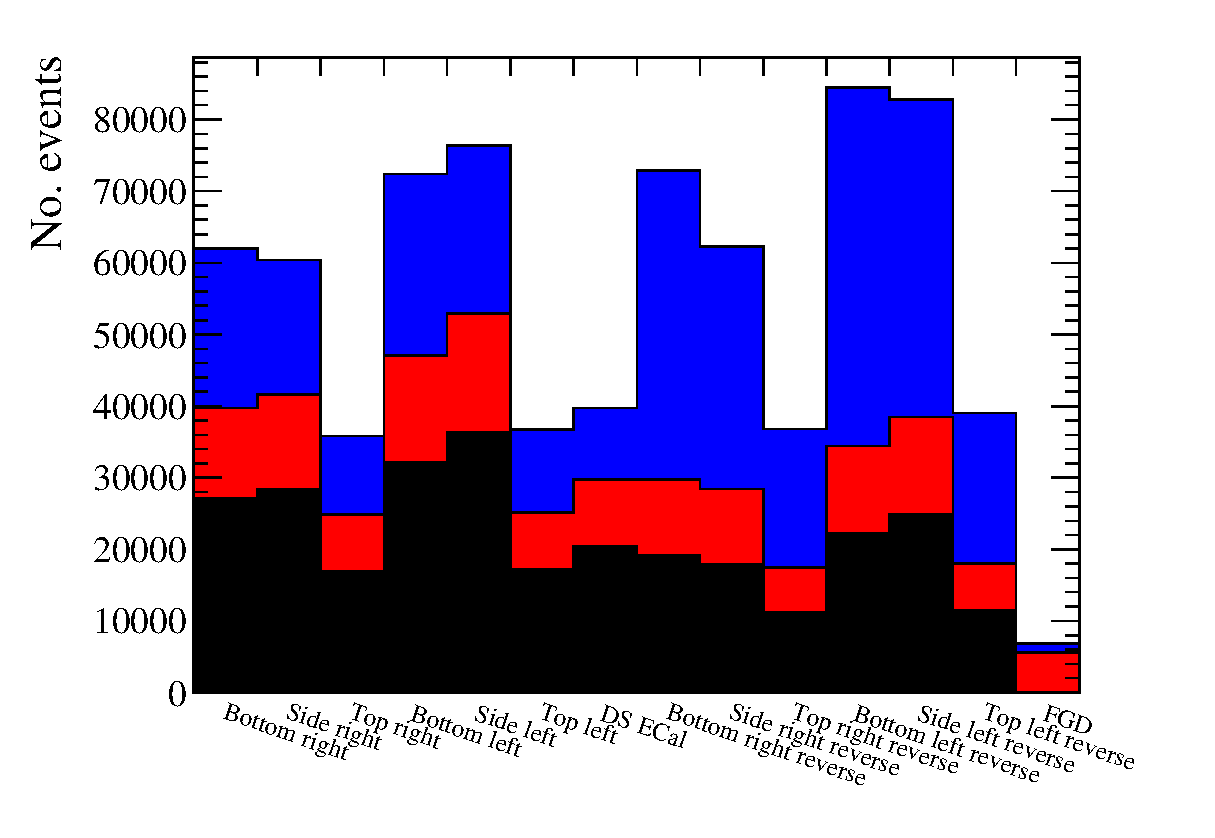
\includegraphics[width=15cm]{images/measurement/rate_fit/MC_Templates_Nominal.eps}
  \caption{The number of events in each input sample separated into the lead (black), carbon (red) and other (blue) templates.\Yoshi{}{ADDRESSED - Should really put the legend in the plot itself. Also say that ``ECal'' is omitted in all but the DS and FGD sample names}.  "ECal" has been omitted in all but the DS-ECal and FGD sample names.}
  \label{fig:NominalMCTemplates}
\end{figure}
\newline
\newline
The underlying fit machinery uses the Minuit2 algorithm provided by the ROOT TFitter framework, chosen primarily because of its ease of use.


\section{Systematic uncertainties}
\label{sec:SystematicUncertainties}
The $\chi^2$ definition shown in equation~\ref{eqn:Chi2Def} allows for systematic uncertainties to be directly included in the fit.  As the systematic uncertainty implementation takes the form of a covariance matrix for the input samples, a good understanding of not only the systematic uncertainties, but how the samples correlate with one another\Yoshi{,}{ADDRESSED - comma} is needed.  
\newline
\newline
As stated above, there are 12 input samples so the covariance matrix will be a 12$\times$12 symmetric matrix.  While it may be obvious that the contents of the matrix will be the covariances of each input sample, it may not be immediately clear what type of covariances are needed.  As described in section~\ref{sec:ECalRateFit}, the algorithm attempts to fit a set of predictions, separated into templates, to a set of measured data samples simultaneously.  The variation comes from the normalisations assigned to each template.  This means that the overall normalisation of the Monte Carlo prediction is free to vary without prior constraint and so \Yoshi{it is the shape difference between the prediction and data that constrains the parameters.}{ADDRESSED - This is an important sentence, so I would reword it with a bit more care; ``shape information between'' doesn't actually mean very much} Therefore the covariance matrix used in the fit should only contain uncertainties which account for the \Yoshi{variations}{ADDRESSED - is better than ``differences'', I think} in the shape of the samples which the systematic sources introduce.
\newline
\newline
The ND280 event simulation \Yoshi{can be}{ADDRESSED - ``is essentially'' is unneeded} broken down into three areas: Simulation of the neutrino flux\Yoshi{;}{ADDRESSED - } simulation of the neutrino interactions\Yoshi{;}{ADDRESSED - } and simulation of the detector response.  No matter how \Yoshi{sophisticated}{ADDRESSED - ``complicated'' is the wrong word} a simulation \Yoshi{is}{ADDRESSED - was can become}, it is unlikely to ever simulate reality with \Yoshi{perfect}{ADDRESSED - ``$100\%$'' is colloquial} accuracy.  The differences between what is simulated (be it flux, interaction or detector) and what happens in nature causes a systematic difference to be seen between collected data and Monte Carlo which must be accounted for.  As the simulation can be broken down into three key areas, the systematic assessment can be \Yoshi{broken down}{ADDRESSED - ``broken down'' appears five times in one page, which is excessive---replace with a few different ways of saying this} into the same three key areas, each of which are presented \Yoshi{below}{ADDRESSED - }.  
\newline
\newline
The actual assessment of a systematic uncertainty can be broken down into two areas: identification of a systematic error source and the propagation of that systematic error source through the analysis.  The identification stage is typically handled by \Yoshi{an official T2K working group}{ADDRESSED - a respective working group} or by an analyser \Yoshi{making use of }{ADDRESSED - with} \Yoshi{data taken outside of the analysis signal region}{ADDRESSED - I would reword ``external sources''} (e.g. control samples).  The propagation of the systematic error source has no strict recipe but it typically involves variation of the identified systematic uncertainty and then either a reweighting of events is applied or the analysis chain is re-run.  The systematic uncertainty treatment used in this analysis uses a \Yoshi{combination of these methods}{ADDRESSED - mixture of the above}.
\newline
\newline
To propagate \Yoshi{effects of the systematic uncertainties,}{ADDRESSED - was systematic uncertainty effect,} a Monte Carlo sample akin to the prediction sample set used in the fit is required.  \Yoshi{Therefore,}{ADDRESSED - So,} a $2.5\times10^{19}$ POT sub sample of beam and \Yoshi{sand Monte Carlo (see section~\ref{sec:MonteCarloSample} for definition)}{ADDRESSED - ``sand Monte Carlo'' is about as jargony as expressions come! Introduce it somewhere before this, and refer the reader there here} is used for this purpose.  All sample systematic covariance matrices are presented as fractional covariance matrices between each of the different detector samples.  For the barrel samples, the selected samples are labelled by their respective module name\Yoshi{,}{ADDRESSED - comma} and the reverse barrel samples (background\Yoshi{-}{ADDRESSED - compound adjective}enriched samples) are labelled with their module name and \Yoshi{`}{ADDRESSED - not '}reverse'.  The assessment of each systematic source is presented individually, resulting in a fractional covariance matrix for that source.  The final systematic covariance matrix is then found by summing all of the individual covariance matrices.
\subsection{Flux systematic evaluation}
\label{subsec:FluxSystematic}
The neutrino flux is one of the core components of the ND280 event simulation and any uncertainties associated with the flux have a direct impact on the measured ND280 event rates.  The associated flux uncertainties can be broken down into four categories\Yoshi{~\cite{PhysRevD.87.012001}}{ADDRESSED - Can this be referenced to one of the beam-related papers?}:
\begin{itemize}
  \item Properties of the proton beam such as profile and alignment
  \item Alignment of the target and focusing horns
  \item The current in the focusing horns and the magnetic field it generates
  \item Hadron production induced by beam interactions with the target
\end{itemize}
As the neutrino flux prediction is so important for all T2K analyses, the flux uncertainties are constrained using a range of measurements.  These include external measurements from the NA61/SHINE collaboration\Yoshi{~\cite{PhysRevC.84.034604}}{A lot of these need citations}, from the proton beam monitors, measurements of a spare magnetic horn and from the INGRID detector.  Measured uncertainties from each source are used to vary the flux in JNUBEAM which produces a covariance matrix for each source.  The covariance matrix to be used by the final analyser is the sum of each covariance matrix which is shown in Fig.~\ref{fig:FluxPredictionSyst}.  The covariance matrix is split into two detector sections: ND280 and SK.  Each detector section is then separated into two beam running modes ($\nu$ and $\bar{\nu}$ runnings) which are also separated into four neutrino flavours ($\nu_\mu$, $\bar{\nu}_\mu$, $\nu_e$ and $\bar{\nu}_e$).  Finally, each neutrino flavour is separated into a set of energy bins.  The presented analysis is a $\nu_\mu$ cross-section measurement using ND280, so only the ND280, $\nu$-running mode section of the covariance matrix needs consideration.
\begin{figure}
  \centering
  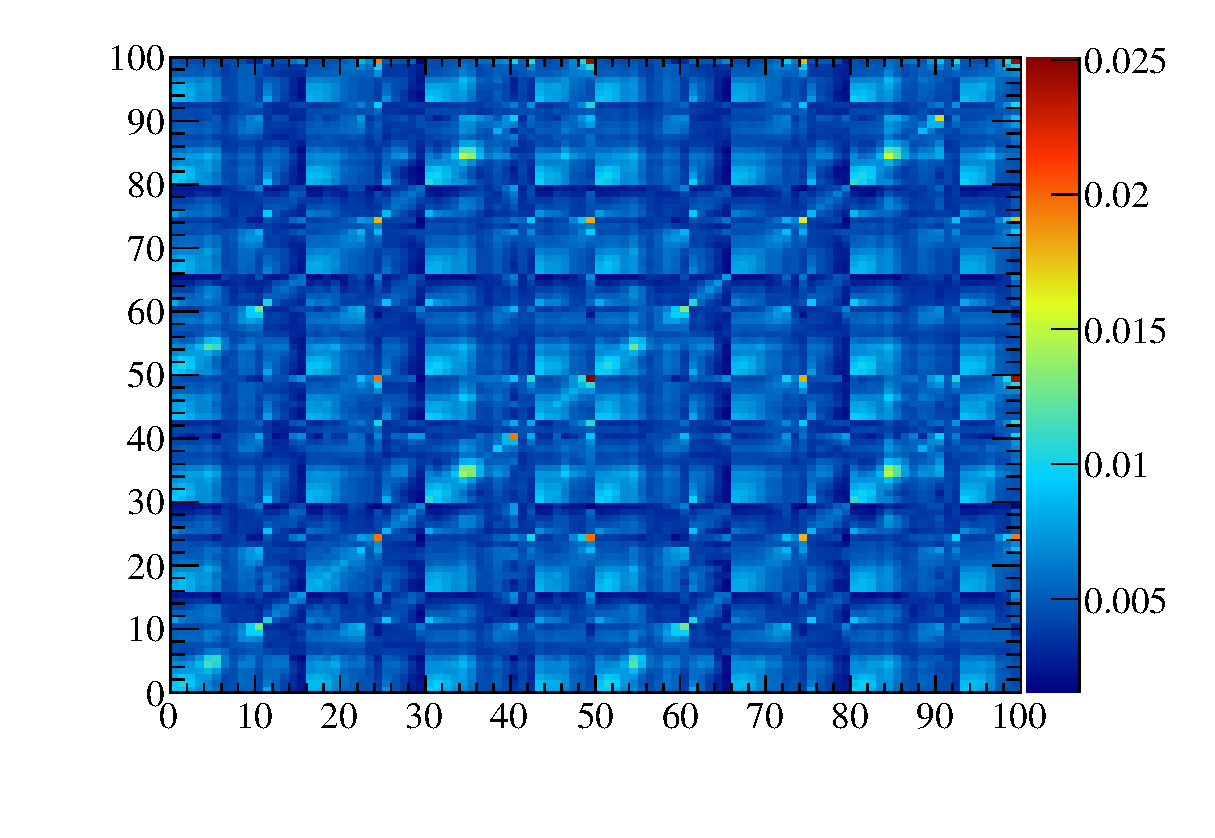
\includegraphics[width=12cm]{images/measurement/systematics/flux/flux_prediction_syst.eps}
  \caption{The flux prediction covariance matrix.  The matrix is binned in detector (SK and ND280), neutrino flavour and energy.}
  \label{fig:FluxPredictionSyst}
\end{figure}
The provided flux covariance matrix is a fractional covariance matrix, binned in neutrino energy and flavour.  As the neutrino energy and flavour information of events seen in this analysis is readily available, the flux covariance matrix can be used to reweight the events in the Monte Carlo sample to propagate the effect of the systematic uncertainty through the analysis.  To do this, the flux covariance matrix is Cholesky decomposed and the resulting matrix multiplied by a vector filled with random throws from a Gaussian of mean 0 and width 1.  Each element in this multiplied vector constitutes a fractional change in the number of a specific neutrino flavour and energy seen in the analysis.  So, the event weightings are generated by adding 1 to each element of this vector.  Every event selected in the sample is then weighted by the correct event weight (in this case defined by the neutrino flavour and energy) and this number of reweighted events is then recorded.  The above description describes a single throw of the flux systematic propagation.  This process is repeated 1000 times to build up the covariance matrix for the sample.  The sample covariance matrix elements are calculated as
\begin{equation}
  V_{\textrm{ab}} = \frac{1}{N^{\textrm{throws}}}\sum^{N^{\textrm{throws}}}_{i=1}\frac{\left(N_{\textrm{a}}^{i} - N_{\textrm{a}}^{\textrm{nom}}\right)\left(N_{\textrm{b}}^{i} - N_{\textrm{b}}^{\textrm{nom}}\right)}{N_{\textrm{a}}^{\textrm{nom}}N_{\textrm{b}}^{\textrm{nom}}},
  \label{eqn:CovarianceMatrixElementDef}
\end{equation}
where $N_{\textrm{a}}^{\textrm{nom}}$ is the number of events seen in the nominal Monte Carlo for sample 'a' and $N^{\textrm{throws}}$ is the number of systematic throws. $N_{\textrm{a}}^{i}$ is generically the number of events seen in sample 'a' for systematic throw $i$, but its definition depends on which kind of covariance matrix is being calculated.  For a shape+normalisation covariance matrix, $N_{\textrm{a}}^{i}$ is defined as 
\begin{equation}
  N_{\textrm{a}}^{i} = N^{i\prime}_{\textrm{a}}, 
  \label{eqn:NVariedDef}
\end{equation}
where $N^{i\prime}_{\textrm{a}}$ is simply the number of events in sample 'a' for throw $i$ after applying the systematic variation.  When considering a shape-only covariance matrix, $N_{\textrm{a}}^{i}$ is 
\begin{equation}
  N_{\textrm{a}}^{i} = N^{i\prime}_{\textrm{a}}\frac{\displaystyle\sum_{j=1}^{12}N_{\textrm{j}}^{\textrm{nom}}}{\displaystyle\sum_{j=1}^{12}N^{i\prime}_{\textrm{j}}}. 
  \label{eqn:NVariedShapeOnlyDef}
\end{equation}
The extra factor on the \Yoshi{right hand side}{ADDRESSED - was RHS} of equation~\ref{eqn:NVariedShapeOnlyDef} conserves the total number of events seen such that there are an equal total number of events before and after applying the systematic variation.  The sample covariance matrices found by applying the above process are shown in Fig.~\ref{fig:FluxCovarianceMatrices}.
\begin{figure}%
  \centering
  \subfloat[Shape+normalisation.]{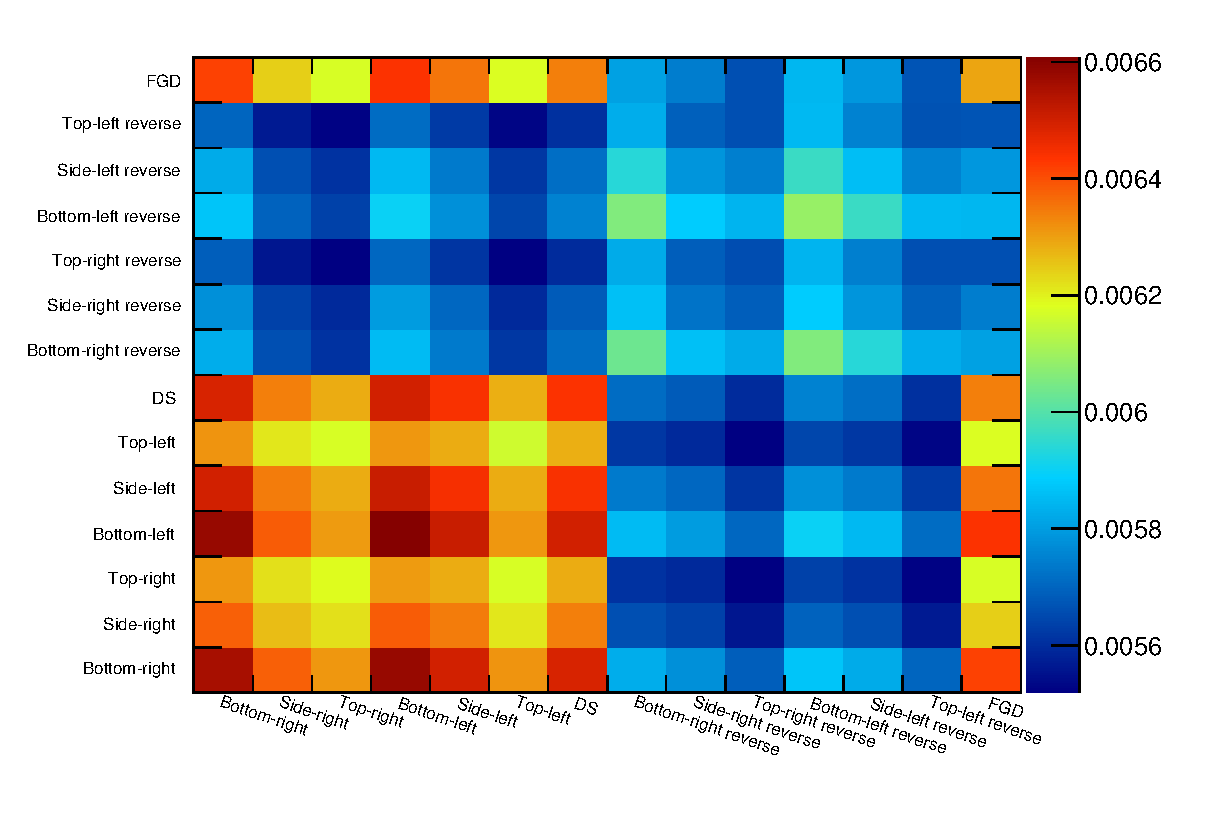
\includegraphics[width=8cm]{images/measurement/systematics/flux/flux_covariance_matrix.eps} \label{fig:FluxShapeNormCovarianceMatrix}}
  \subfloat[Shape-only.]{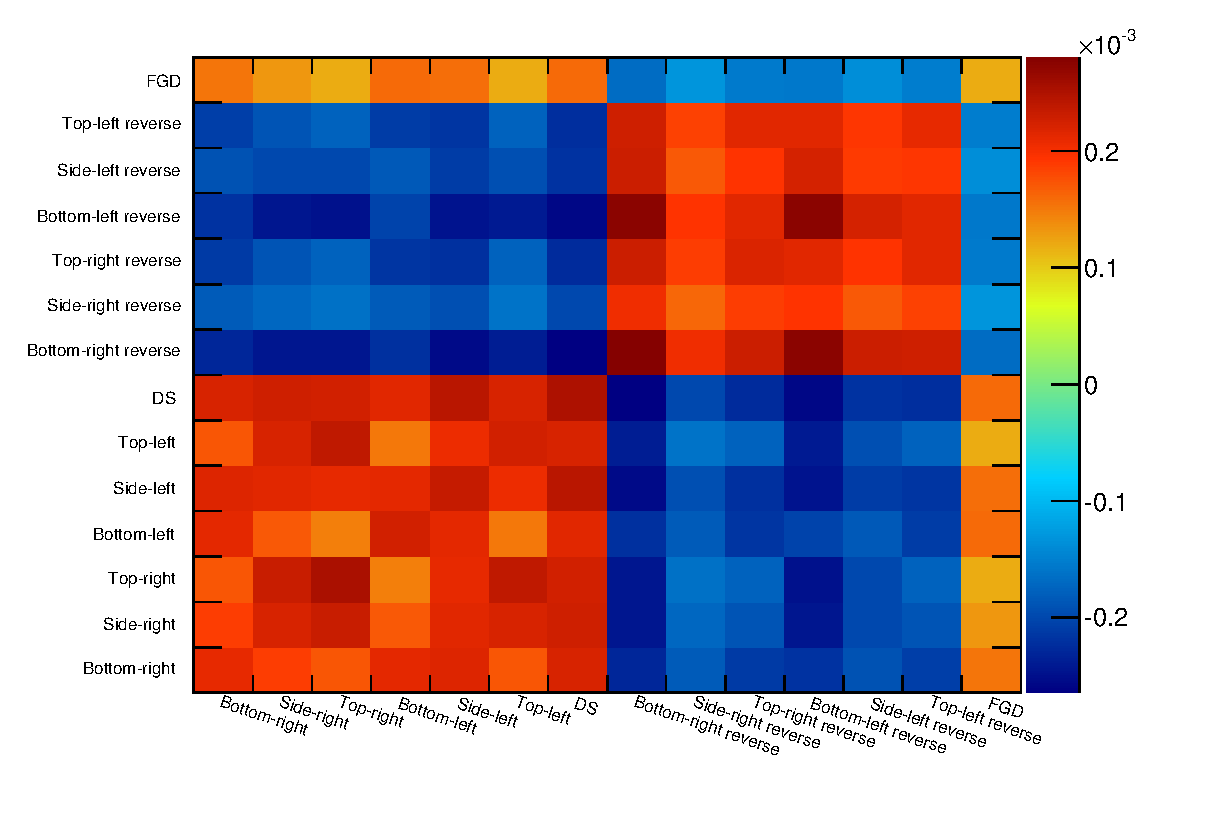
\includegraphics[width=8cm]{images/measurement/systematics/flux/flux_shape_covariance_matrix.eps} \label{fig:FluxShapeOnlyCovarianceMatrix}}
  \caption{The sample covariance induced by the flux uncertainties.}
  \label{fig:FluxCovarianceMatrices}
\end{figure}
\newline
\newline
The effect of the flux systematic on the selection efficiency of lead interactions was also evaluated.  As the main target used in this analysis is the DS ECal, the efficiency variation was evaluated for this detector only.  For each systematic throw described above, the selection efficiency was calculated and recorded.  By plotting the efficiency for each throw, the width of the efficiency distribution can be found which gives the efficiency uncertainty induced by the flux systematic.  This efficiency uncertainty was found to be 0.00097.  The lead selection efficiency in the DS ECal is nominally 0.539, which implies a fractional change of 0.18$\%$, which is essentially negligible.
\begin{figure}
  \centering
  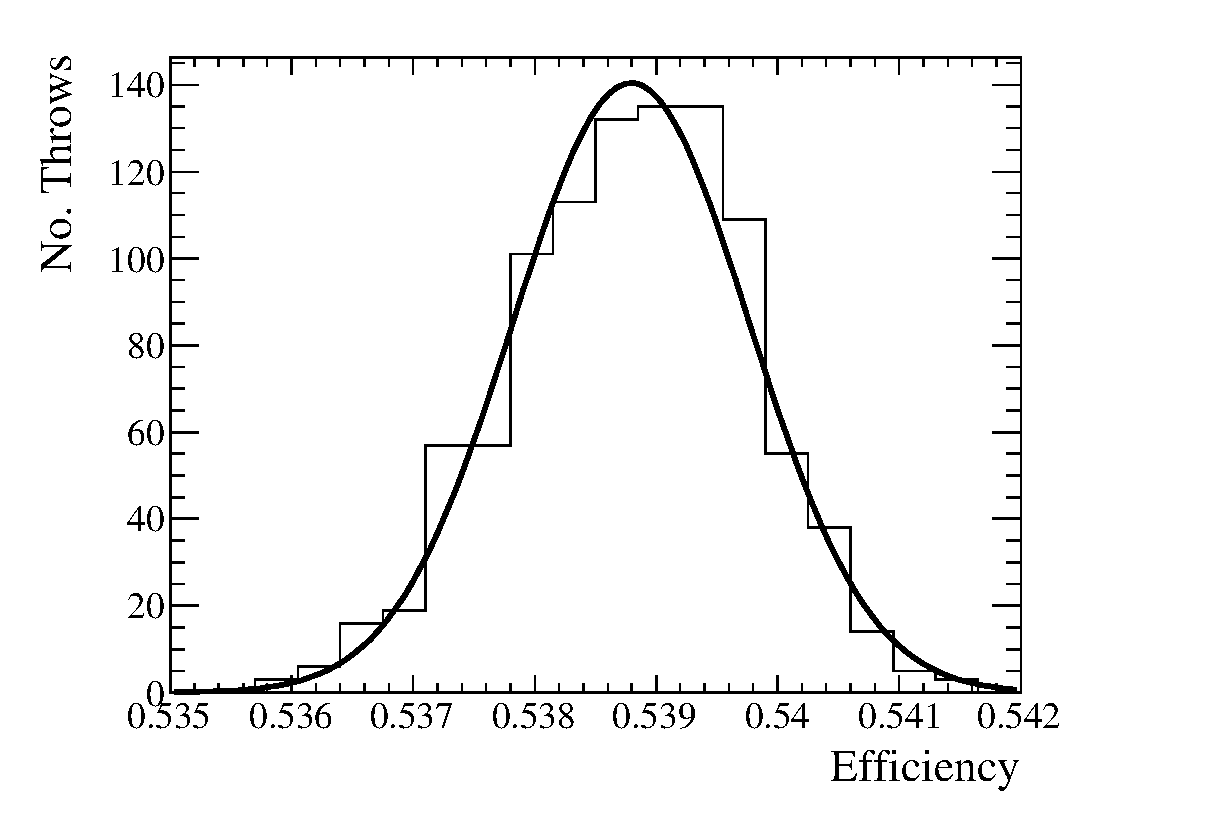
\includegraphics[width=12cm]{images/measurement/systematics/flux/flux_efficiency_variation.eps}
  \caption{The variation in the selection efficiency of lead interactions in the DS ECal caused by the flux systematic.}
  \label{fig:FluxEfficiencyVariation}
\end{figure}
\subsection{Cross-section systematic evaluation}
\label{subsec:CrossSectionSystematic}
The neutrino cross-section picture is still a very much open area of research.  The interaction model used by current neutrino interaction generators use a set of empirical parameters which are tuned on experimental results.  Uncertainties on any one of these empirical parameters will alter the simulated cross-section and thus the event rate seen in the ND280 simulation.  A dedicated working group handles the assessment of the empirical parameters and their corresponding uncertainties.  The parameter uncertainties are given as a covariance matrix along with the known correlations which is shown in Fig.~\ref{fig:XSecPredictionSyst}.  The interaction parameter assessment is chiefly undertaken with the T2K oscillation analyses in mind which means that the nuclear model parameters are only considered for carbon and oxygen.  In the presented analysis, iron and aluminium are two major sources of background interactions which must also be treated in the systematic assessment.  The chosen treatment is to assign a data-motivated, normalisation uncertainty to such backgrounds.  The iron uncertainty is taken from the iron cross-section measurement using INGRID~\cite{PhysRevD.90.052010}.  The aluminium uncertainty is taken from the total $\nu_\mu$ cross-section on aluminium measurement using the IHEP-JINR detector~\cite{Anikeev:1995dj}.  The IHEP-JINR detector was exposed to a neutrino beam with a 3~GeV to 30~GeV energy range which is samples a higher energy than the T2K neutrino beam.  Because of this fact, it was decided to double the quoted aluminium cross-section uncertainty.  As element specific parameters for lead do not appear in Fig.~\ref{fig:XSecPredictionSyst}, such parameters are additionally assessed separately using NEUT.
\begin{figure}
  \centering
  %INSERT XSEC COVARIANCE MATRIX
  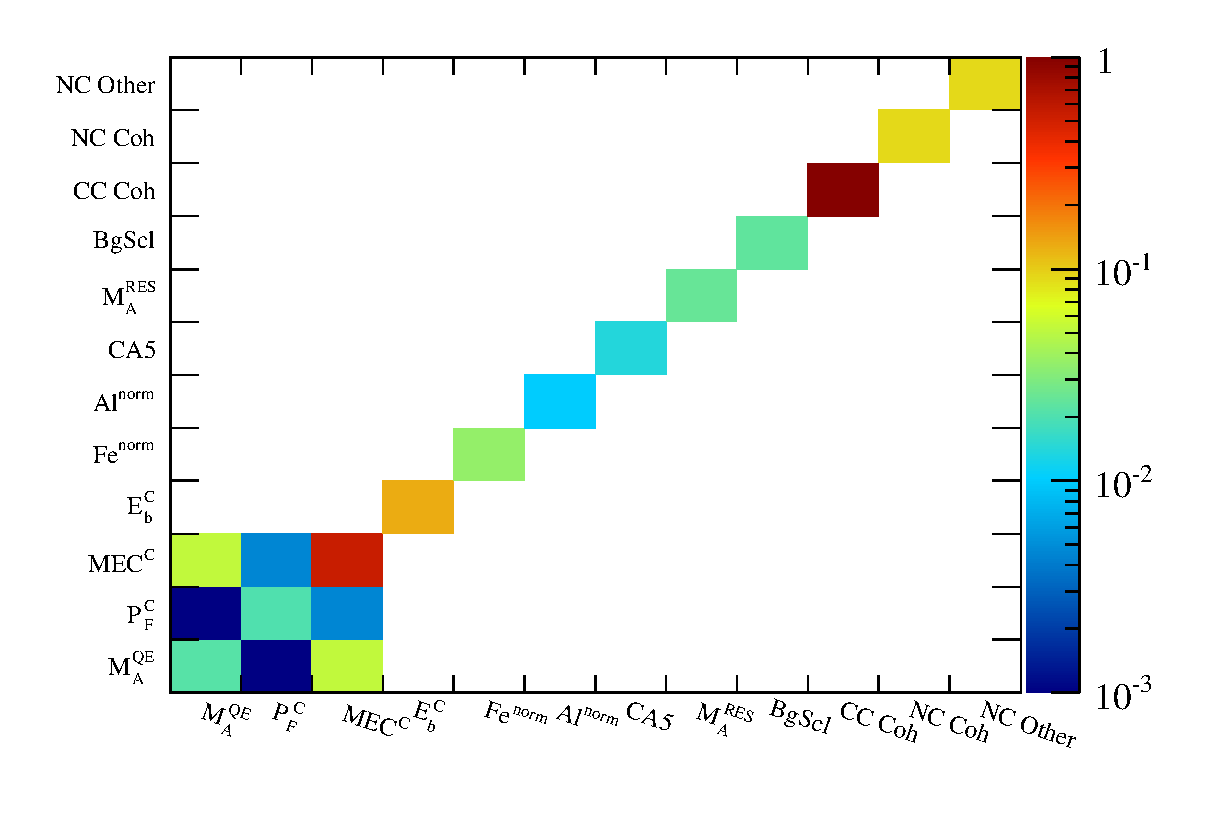
\includegraphics[width=12cm]{images/measurement/systematics/xsec/xsec_prediction_syst.eps}
  \caption{The neutrino cross-section model covariance matrix.}
  \label{fig:XSecPredictionSyst}
\end{figure}
\newline
\newline
To propagate the effect of the cross-section systematic through the analysis, the covariance matrix shown in Fig.~\ref{fig:XSecPredictionSyst} was Cholesky decomposed and the resultant matrix multiplied by a vector of random numbers thrown from a Gaussian (the same approach as described in section~\ref{subsec:FluxSystematic}).  However, the re-weighting in this case is more complicated.  The T2KReWeight~\cite{T2KReWeightTN} software takes the parameters errors from the throw along with the simulated NEUT vertex which is matched to the event being varied.  T2KReWeight then calculates a weight based on the inputted errors and the NEUT vertex in question.  Using the T2KReWeight machinery, 1000 systematic throws from the covariance matrix shown in Fig.~\ref{fig:XSecPredictionSyst} were made and sample covariance matrices were calculated, which are shown in Fig.~\ref{fig:XSecCovarianceMatrices}.
\begin{figure}[t!]
  \centering
  \subfloat[Shape+normalisation.]{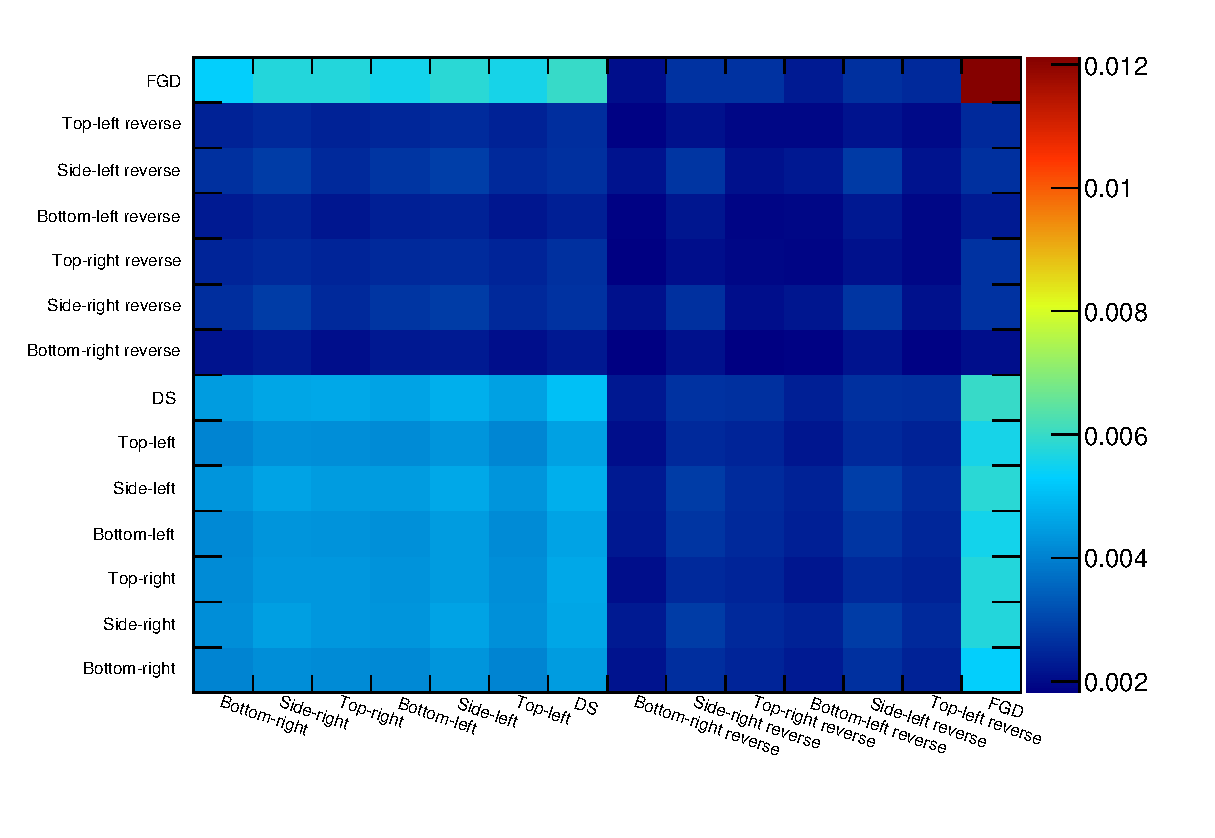
\includegraphics[width=8cm]{images/measurement/systematics/xsec/xsec_covariance_matrix.eps} \label{fig:XSecShapeNormCovarianceMatrix}}
  \subfloat[Shape-only.]{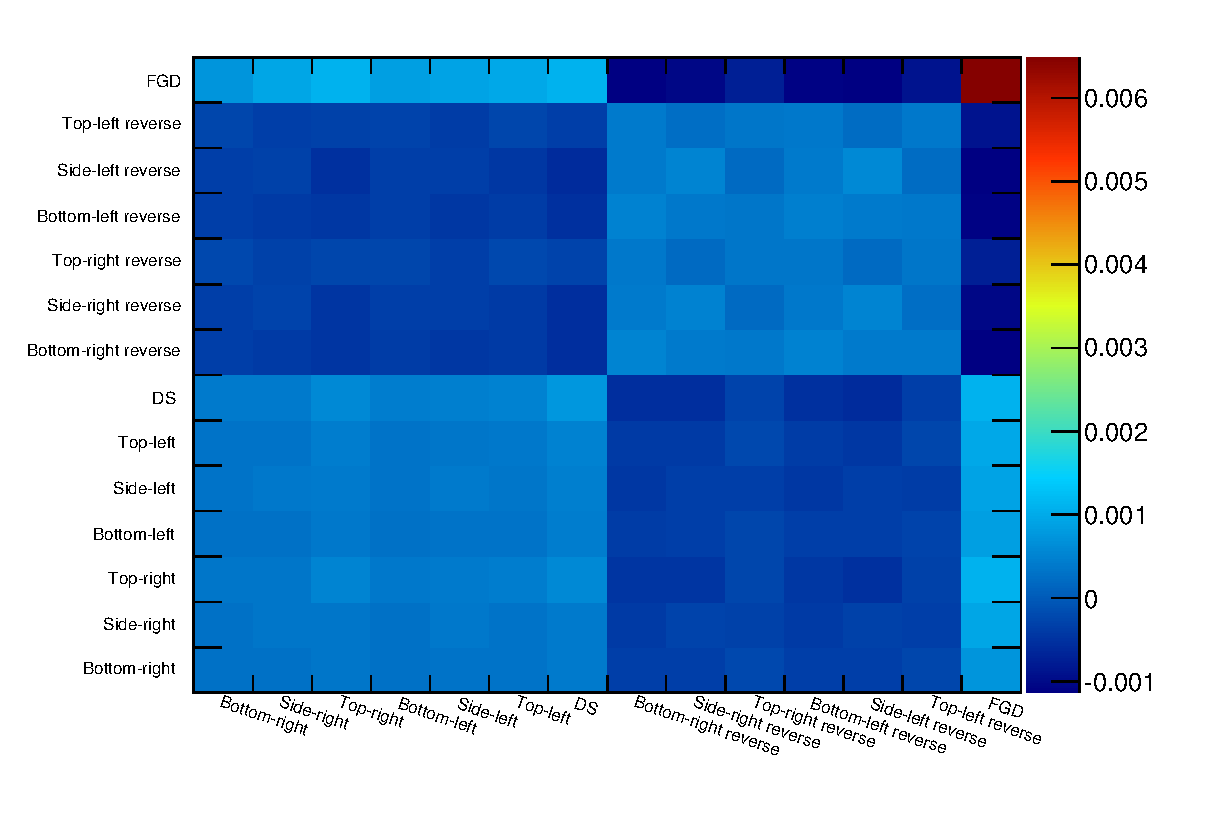
\includegraphics[width=8cm]{images/measurement/systematics/xsec/xsec_shape_covariance_matrix.eps} \label{fig:XSecShapeOnlyCovarianceMatrix}}
  \caption{The sample covariance induced by the cross-section model uncertainties.}
  \label{fig:XSecCovarianceMatrices}
\end{figure}
\newline
\newline
As with the flux systematic, the uncertainty in the selection efficiency for lead interactions in the DS ECal due to the cross-section model systematic was found by recording the efficiency for each throw.  The variation in the efficiency is shown in Fig.~\ref{fig:XSecEfficiencyVariation}.  The efficiency uncertainty was found to be 0.001 which corresponds to a 0.2$\%$ error which is, again, negligible.
\begin{figure}[b!]
  \centering
  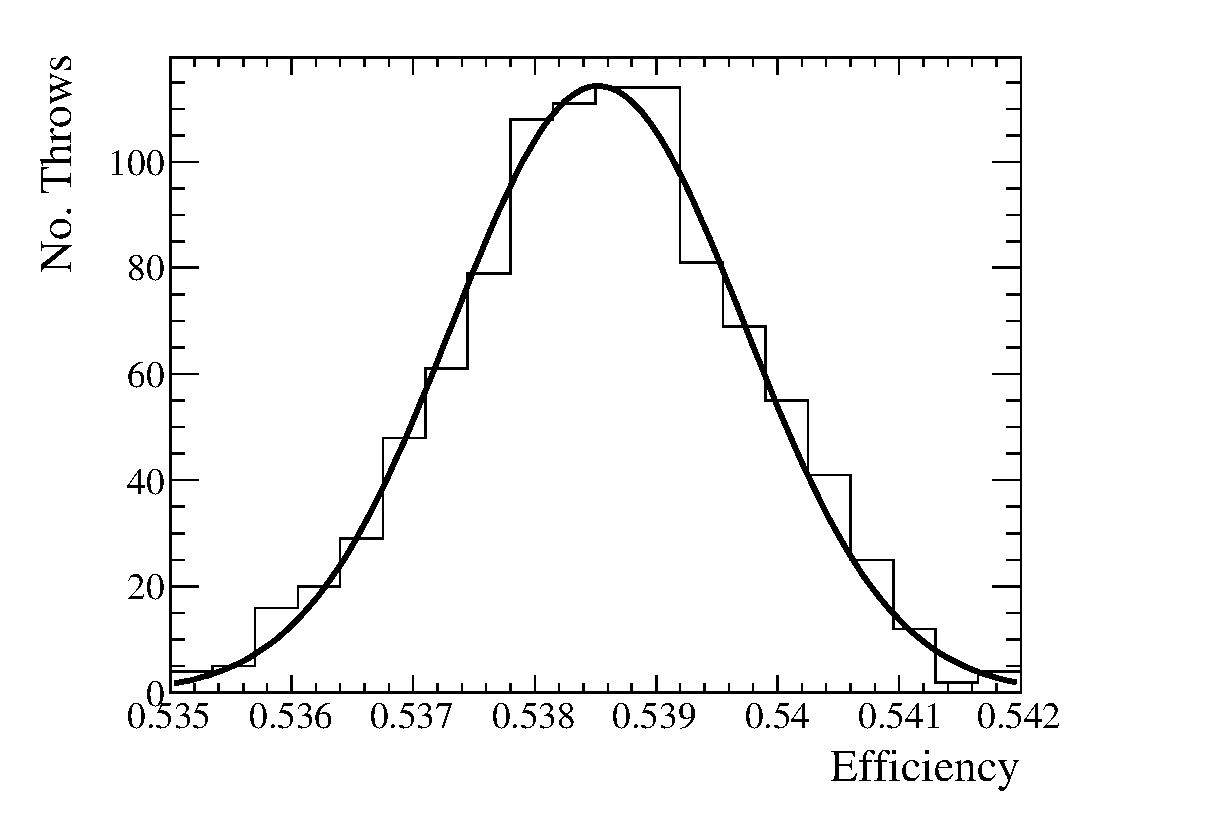
\includegraphics[width=10cm]{images/measurement/systematics/xsec/xsec_efficiency_variation.eps}
  \caption{The variation in the selection efficiency of lead interactions in the DS ECal caused by the cross-section model systematic.}
  \label{fig:XSecEfficiencyVariation}
\end{figure}
\newline
\newline
As discussed above, the re-weighting of element specific parameters for events matched to lead interactions was not possible using T2KReWeight.  As meson-exchange current interactions for lead interactions are not implemented in NEUT, the only parameters necessary to vary are $P_{\textrm{F}}^{\textrm{Pb}}$ and $E_{\textrm{b}}^{\textrm{Pb}}$ which are the Fermi-momentum and binding energy for lead respectively.  So, NEUT was used to produce 10,000 neutrino interactions on lead with uniform energy between 0~GeV and 10~GeV for the nominal parameters and $\pm\upsigma$ variations of the parameters.  The associated uncertainties were not readily available in the literature so 1.5 times the carbon parameter uncertainties were used as a conservative estimate.  The NEUT events were used to plot the ratio of the varied cross-section to the nominal cross-section as a function of energy.  The ratios for $P_{\textrm{F}}^{\textrm{Pb}}$ and $E_{\textrm{b}}^{\textrm{Pb}}$ are shown in Fig.~\ref{fig:PbXSecPfRatio} and Fig.~\ref{fig:PbXSecEbRatio} respectively.  The variation in the cross-section caused by variation in $E_{\textrm{b}}^{\textrm{Pb}}$ is sub-percent so there should be a negligible variation in the event rate which means this can be ignored.  However, there is significant variation in the cross-section at low energy due to variations in $P_{\textrm{F}}^{\textrm{Pb}}$ so this effect must be propagated through the analysis.  To do this, the ratio distributions shown in Fig.~\ref{fig:PbXSecPfRatio} were treated as a set of events weights.  The $+\upsigma$ and $-\upsigma$ weights were applied to the sample separately, creating two systematic throws.  The results of the systematic throws were used to generate the sample covariances, which are shown in Fig.~\ref{fig:PbXSecCovarianceMatrices}.
\begin{figure}%
  \centering
  \subfloat[$P_{\textrm{F}}^{\textrm{Pb}}$]{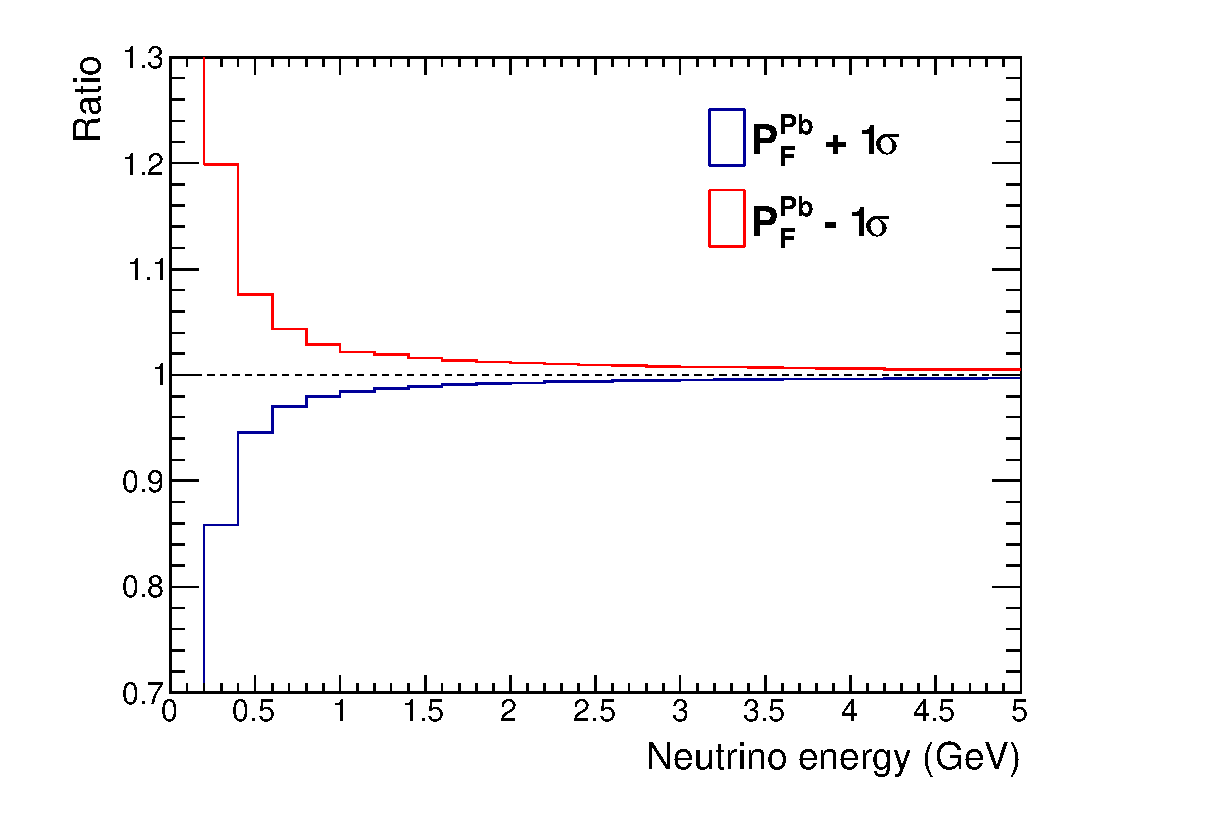
\includegraphics[width=8cm]{images/measurement/systematics/xsec/pbxsec_pf_ratio.eps} \label{fig:PbXSecPfRatio}}
  \subfloat[$E_{\textrm{b}}^{\textrm{Pb}}$]{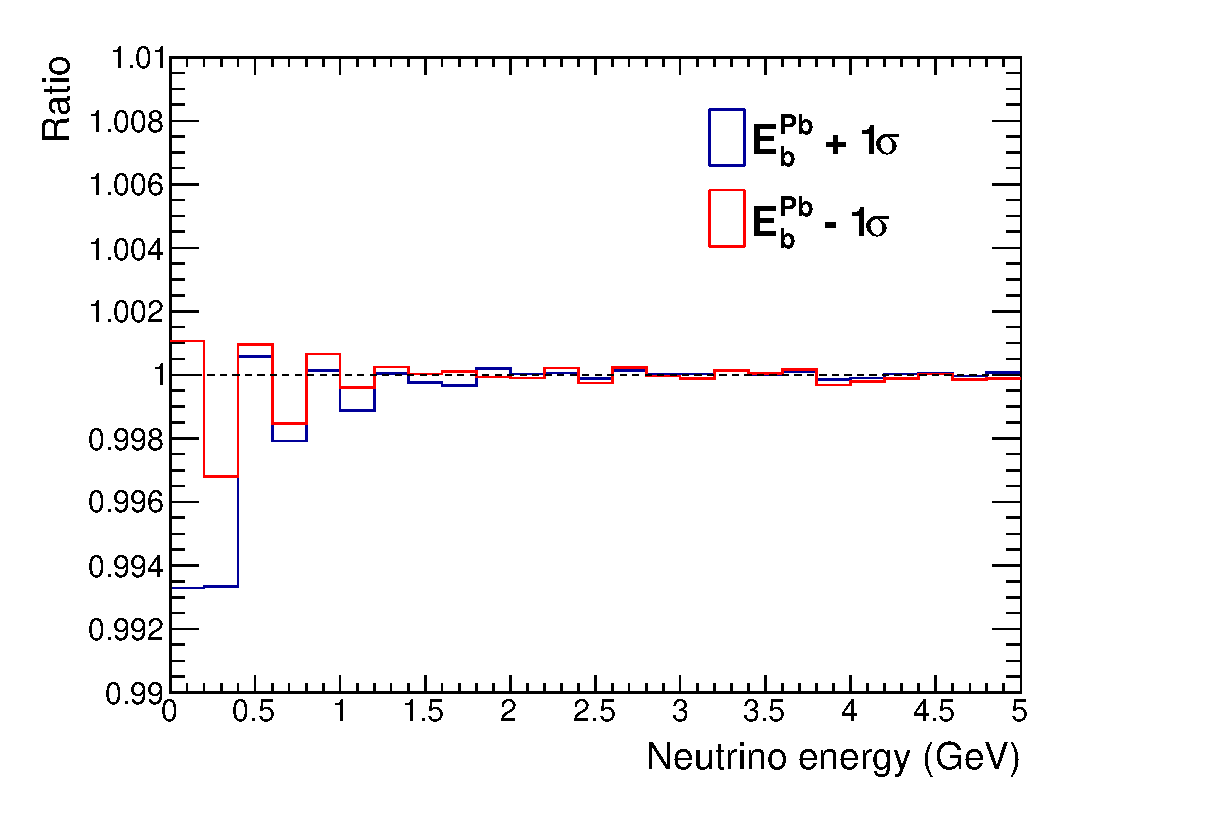
\includegraphics[width=8cm]{images/measurement/systematics/xsec/pbxsec_eb_ratio.eps} \label{fig:PbXSecEbRatio}}
  \caption{The ratio of the $\pm$$\upsigma$ cross-section to the nominal cross-section for lead as a function of neutrino energy.  Distributions produced by W. Ma.}
  \label{fig:PbXSecRatios}
\end{figure}
\begin{figure}%
  \centering
  \subfloat[Shape+normalisation.]{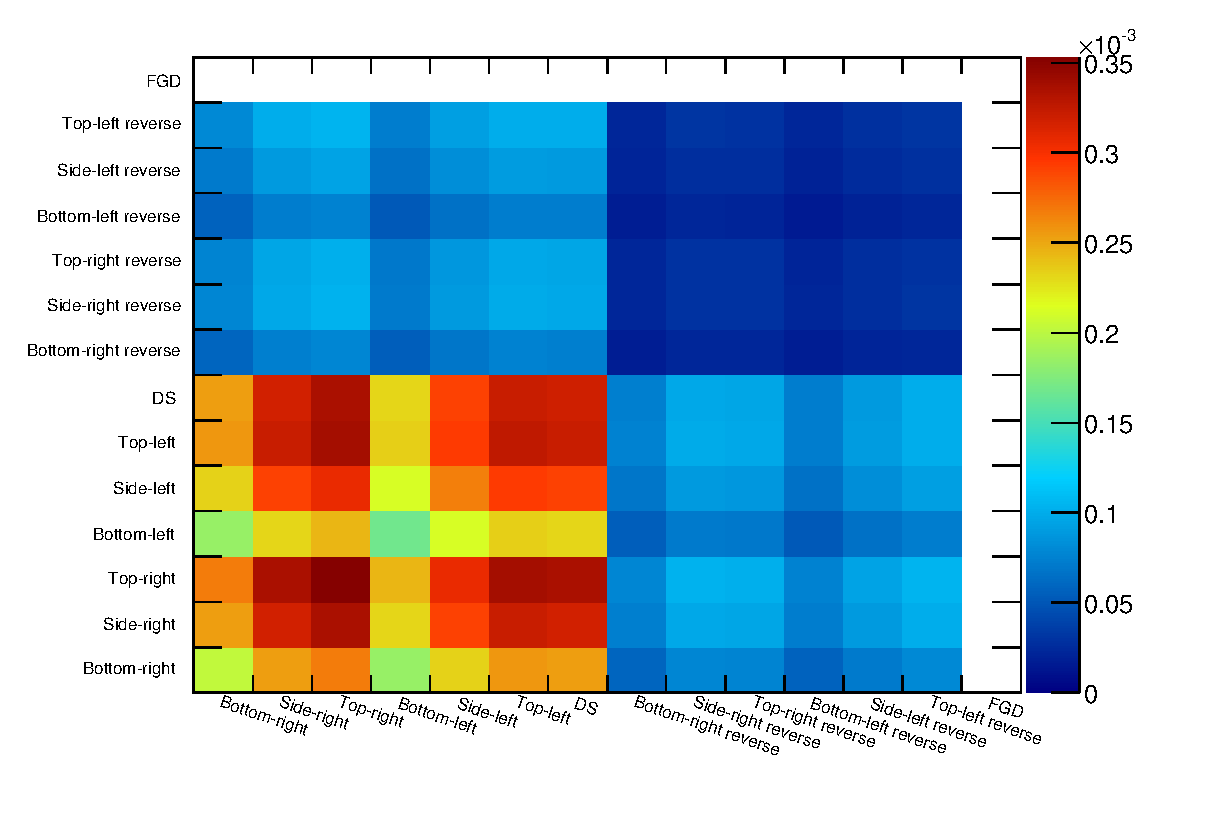
\includegraphics[width=8cm]{images/measurement/systematics/xsec/pb_xsec_covariance_matrix.eps} \label{fig:PbXSecShapeNormCovarianceMatrix}}
  \subfloat[Shape-only.]{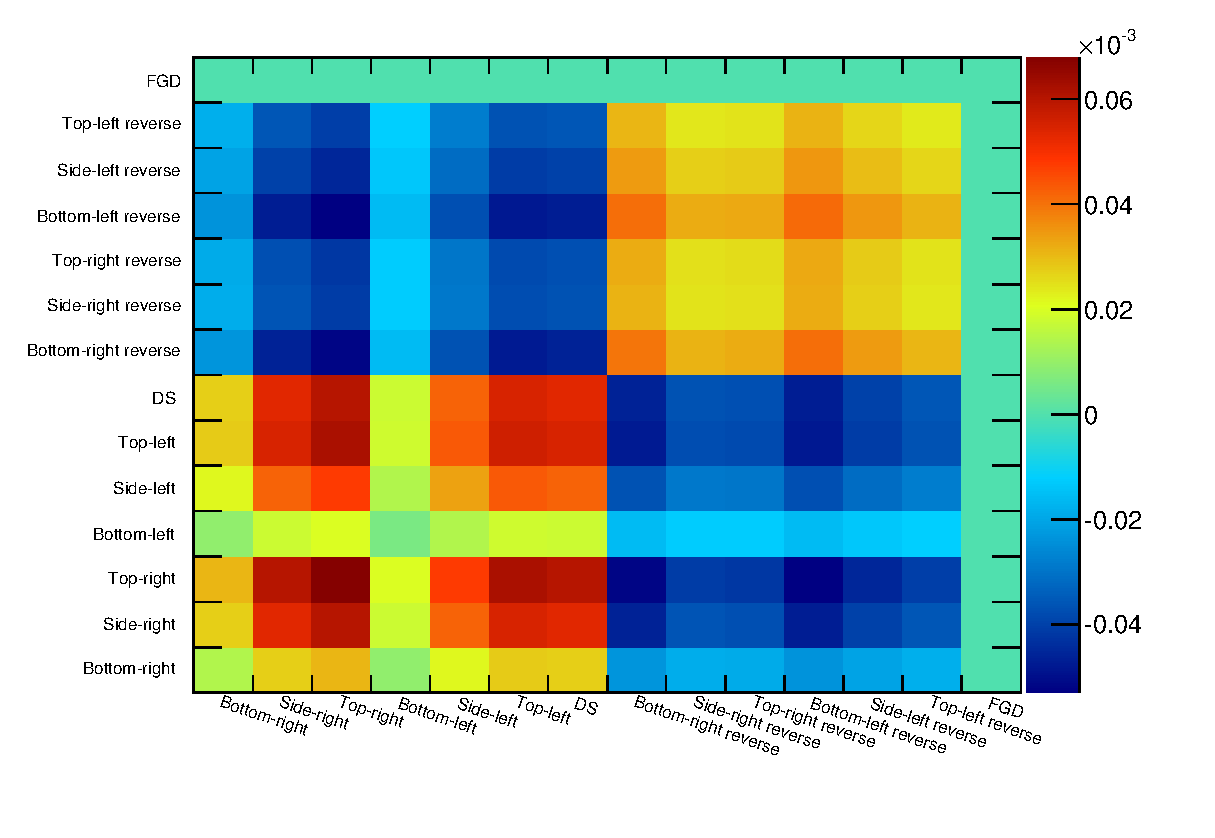
\includegraphics[width=8cm]{images/measurement/systematics/xsec/pb_xsec_shape_covariance_matrix.eps} \label{fig:PbXSecShapeOnlyCovarianceMatrix}}
  \caption{The sample covariance induced by variation of $P_{\textrm{F}}^{\textrm{Pb}}$.}
  \label{fig:PbXSecCovarianceMatrices}
\end{figure}
\newline
\newline
Final-state interactions (FSI) within the nucleus after a neutrino interaction has occurred could also cause a variation in the event rate.  While the selection used in this analysis is CC inclusive, the method used separates events out into prong topologies.  Any uncertainty in the FSI could cause migration of events from one prong topology to another.  The Neutrino Interaction Working Group (NIWG) assesses these uncertainties and provides a set of parameters for an analyser to vary, all of which are associated with $\pi^{\pm}$ interactions.  There are six parameters associated with FSI:
\begin{itemize}
  \item Low energy quasi-elastic scattering (FSIQEL)
  \item High energy quasi-elastic scattering (FSIQEH)
  \item Pion production (FSIINEL)
  \item Pion absorption (FSIABS)
  \item Low energy single charge exchange (FSICXL)
  \item High energy single charge exchange (FSICXH)
\end{itemize}
The NIWG provides combinations of the $1\upsigma$ errors for the parameters highlighted above which span the whole FSI parameter space.  The errors are provided as weights in 16 parameters sets which represent the $1\upsigma$ contour for the FSI parameter space and are shown in table~\ref{table:FSIErrors}.  Each parameter set can be used to generate one systematic throw, by passing the parameters to T2KReWeight and subsequently re-weighting the events.  As with the cross-section model systematics described above, the parameter variations only affect carbon and oxygen.  The FSI systematic throws were used to generate the sample covariance matrices which are shown in Fig.~\ref{fig:FSICovarianceMatrices}.
%\newline
%\newline
%It is not trivial how to assess how the FSI uncertainties affect the lead interactions as the T2KReWeight machinery can not be used.  FSI should cause a mixing between the different CC interaction final states which means that there will be migration from one prong topology to another.  Based on the efficiencies in table~\ref{table:SelEfficiency}, the main concern would be from 2 prong topology events migrating to 1 prong topology events in the barrel where such events would be exposed to a stream of cuts which are 12$\%$ less efficient.  Assuming that the variation in event rate induced by the FSI variation for carbon/oxygen is similar for lead, the change in events seen would be 
\begin{table}
  \begin{tabular}{ c c c c c c c }
    Parameter set & FSIQEL & FSIQEH & FSIINEL & FSIABS & FSICXL & FSICXH \\ \hline \hline
    Nominal & 1.0 & 1.8 & 1.0 & 1.1 & 1.0 & 1.8 \\
    15 & 0.6 & 1.1 & 1.5 & 0.7 & 0.5 & 2.3 \\
    16 & 0.6 & 1.1 & 1.5 & 0.7 & 1.6 & 2.3 \\
    17 & 0.7 & 1.1 & 1.5 & 1.6 & 0.4 & 2.3 \\
    18 & 0.7 & 1.1 & 1.5 & 1.6 & 1.6 & 2.3 \\
    19 & 1.4 & 1.1 & 1.5 & 0.6 & 0.6 & 2.3 \\
    20 & 1.3 & 1.1 & 1.5 & 0.7 & 1.6 & 2.3 \\
    21 & 1.5 & 1.1 & 1.5 & 1.5 & 0.4 & 2.3 \\
    22 & 1.6 & 1.1 & 1.5 & 1.6 & 1.6 & 2.3 \\
    23 & 0.6 & 2.3 & 0.5 & 0.7 & 0.5 & 1.3 \\
    24 & 0.6 & 2.3 & 0.5 & 0.7 & 1.6 & 1.3 \\
    25 & 0.7 & 2.3 & 0.5 & 1.6 & 0.4 & 1.3 \\
    26 & 0.7 & 2.3 & 0.5 & 1.6 & 1.6 & 1.3 \\
    27 & 1.4 & 2.3 & 0.5 & 0.6 & 0.6 & 1.3 \\
    28 & 1.3 & 2.3 & 0.5 & 0.7 & 1.6 & 1.3 \\
    29 & 1.5 & 2.3 & 0.5 & 1.5 & 0.4 & 1.3 \\
    30 & 1.6 & 2.3 & 0.5 & 1.6 & 1.6 & 1.3 \\
  \end{tabular}
  \caption{FSI parameters, provided by the NIWG, representing the $1\upsigma$ contour in the FSI parameter space~\cite{NIWGErrorTN}.}
  \label{table:FSIErrors}
\end{table}
\begin{figure}%
  \centering
  \subfloat[Shape+normalisation.]{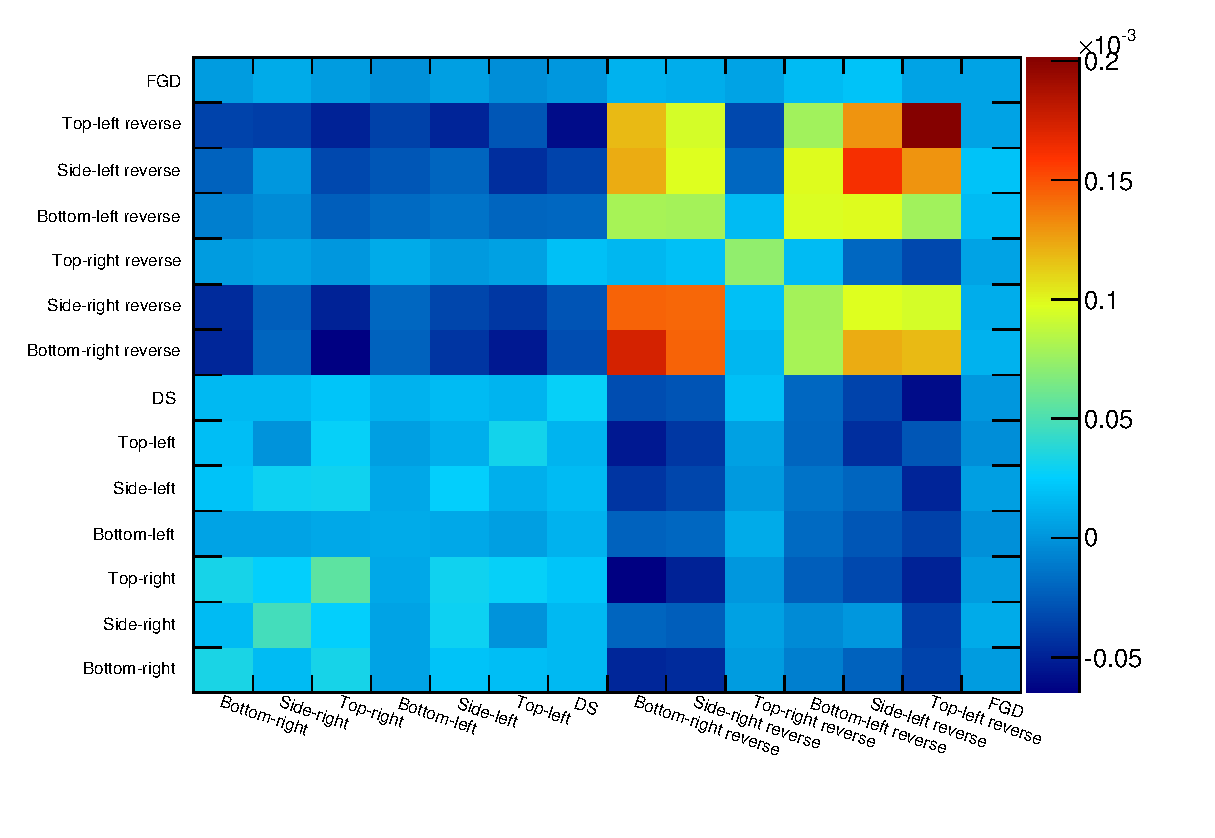
\includegraphics[width=8cm]{images/measurement/systematics/xsec/fsi_covariance_matrix.eps} \label{fig:FSIShapeNormCovarianceMatrix}}
  \subfloat[Shape-only.]{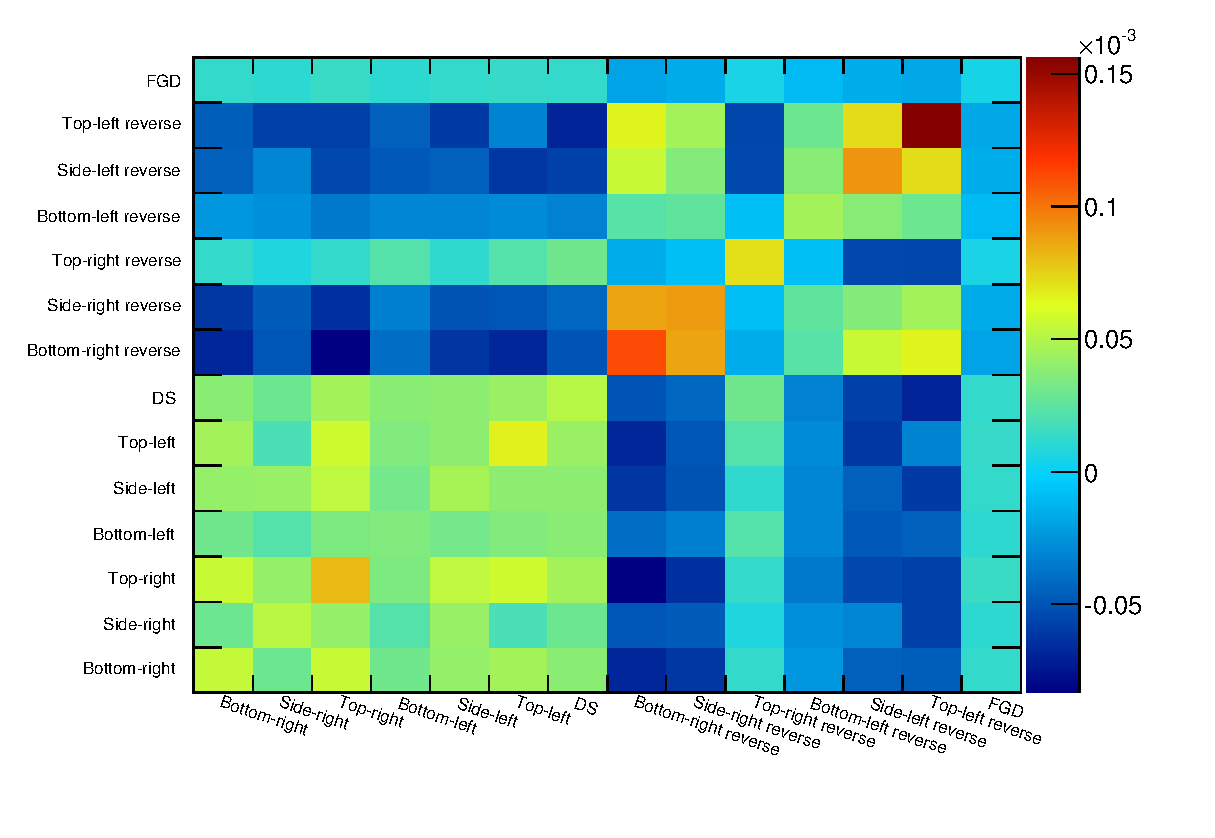
\includegraphics[width=8cm]{images/measurement/systematics/xsec/fsi_shape_covariance_matrix.eps} \label{fig:FSIShapeOnlyCovarianceMatrix}}
  \caption{The sample covariance induced by variation of of the FSI parameters outlined in table~\ref{table:FSIErrors}.}
  \label{fig:FSICovarianceMatrices}
\end{figure}
%really is just the number of in sample a for throw $i$ after applying the event weights.  For the shape-only covariance matrix, $N_{\textrm{a}}^{i}$ is defined as 
%\begin{equation}
%  N_{\textrm{a}}^{i} = 
%\end{equation}
\subsection{ECal detector systematic evaluation}
\label{subsec:ECalDetectorSystematic}
The analysis presented makes heavy use of a computational model of the ND280 ECal.  Any differences between this model and the real ND280 ECal could cause a systematic difference between the analysed Monte Carlo and the collected data used in this study.  So, several key areas have been identified which could cause such a systematic discrepancy, under the assumption that the differences exist.
\newline
\newline
The implemented selections uses the enhanced reconstruction, outlined in chapter~\ref{chap:EnhancedECalReconstruction}.  The enhanced reconstruction depends on a set of clustering algorithms which are outlined in section~\ref{sec:ECalEventReconstruction} and those clustering algorithms depend on the hit scintillator bars themselves.  Following this trail back, it can be argued that the vast majority of the ECal detector systematics can be covered by assessing the ability of the ECal to reconstruct individual hits.  Specifically, the vast majority of the ECal's systematic uncertainties can be assessed by investigating the hit efficiency of the scintillator bars.  
\newline
\newline
The aim of this study is to quantify the relative ECal hit inefficiency of collected data when compared to MC and use that information to invoke a similar ECal hit inefficiency in the MC.  The effect of the hit inefficiency can then be propagated through the reconstruction and analysis to study its effect on the number of selected events.  Fig.~\ref{fig:LayerEfficiencyCosmicData} shows the layer-by-layer efficiency of the ND280 ECals, measured using cosmic data~\cite{1748-0221-8-10-P10019}.  Cosmic rays, which are largely composed of MIPs, are typically through going and only hit one bar per layer.  So, the efficiencies shown in Fig.~\ref{fig:LayerEfficiencyCosmicData}, can be used as a proxy for the hit efficiency of the scintillator bars.  Fig.~\ref{fig:LayerEfficiencyCosmicData} contains almost all of the necessary information required to study this systematic uncertainty with the only missing information being the hit efficiency of the MC ECal.  Due to time constraints, it was necessary to make a couple of conservative assumptions:
\begin{figure}[t!]
  \centering
  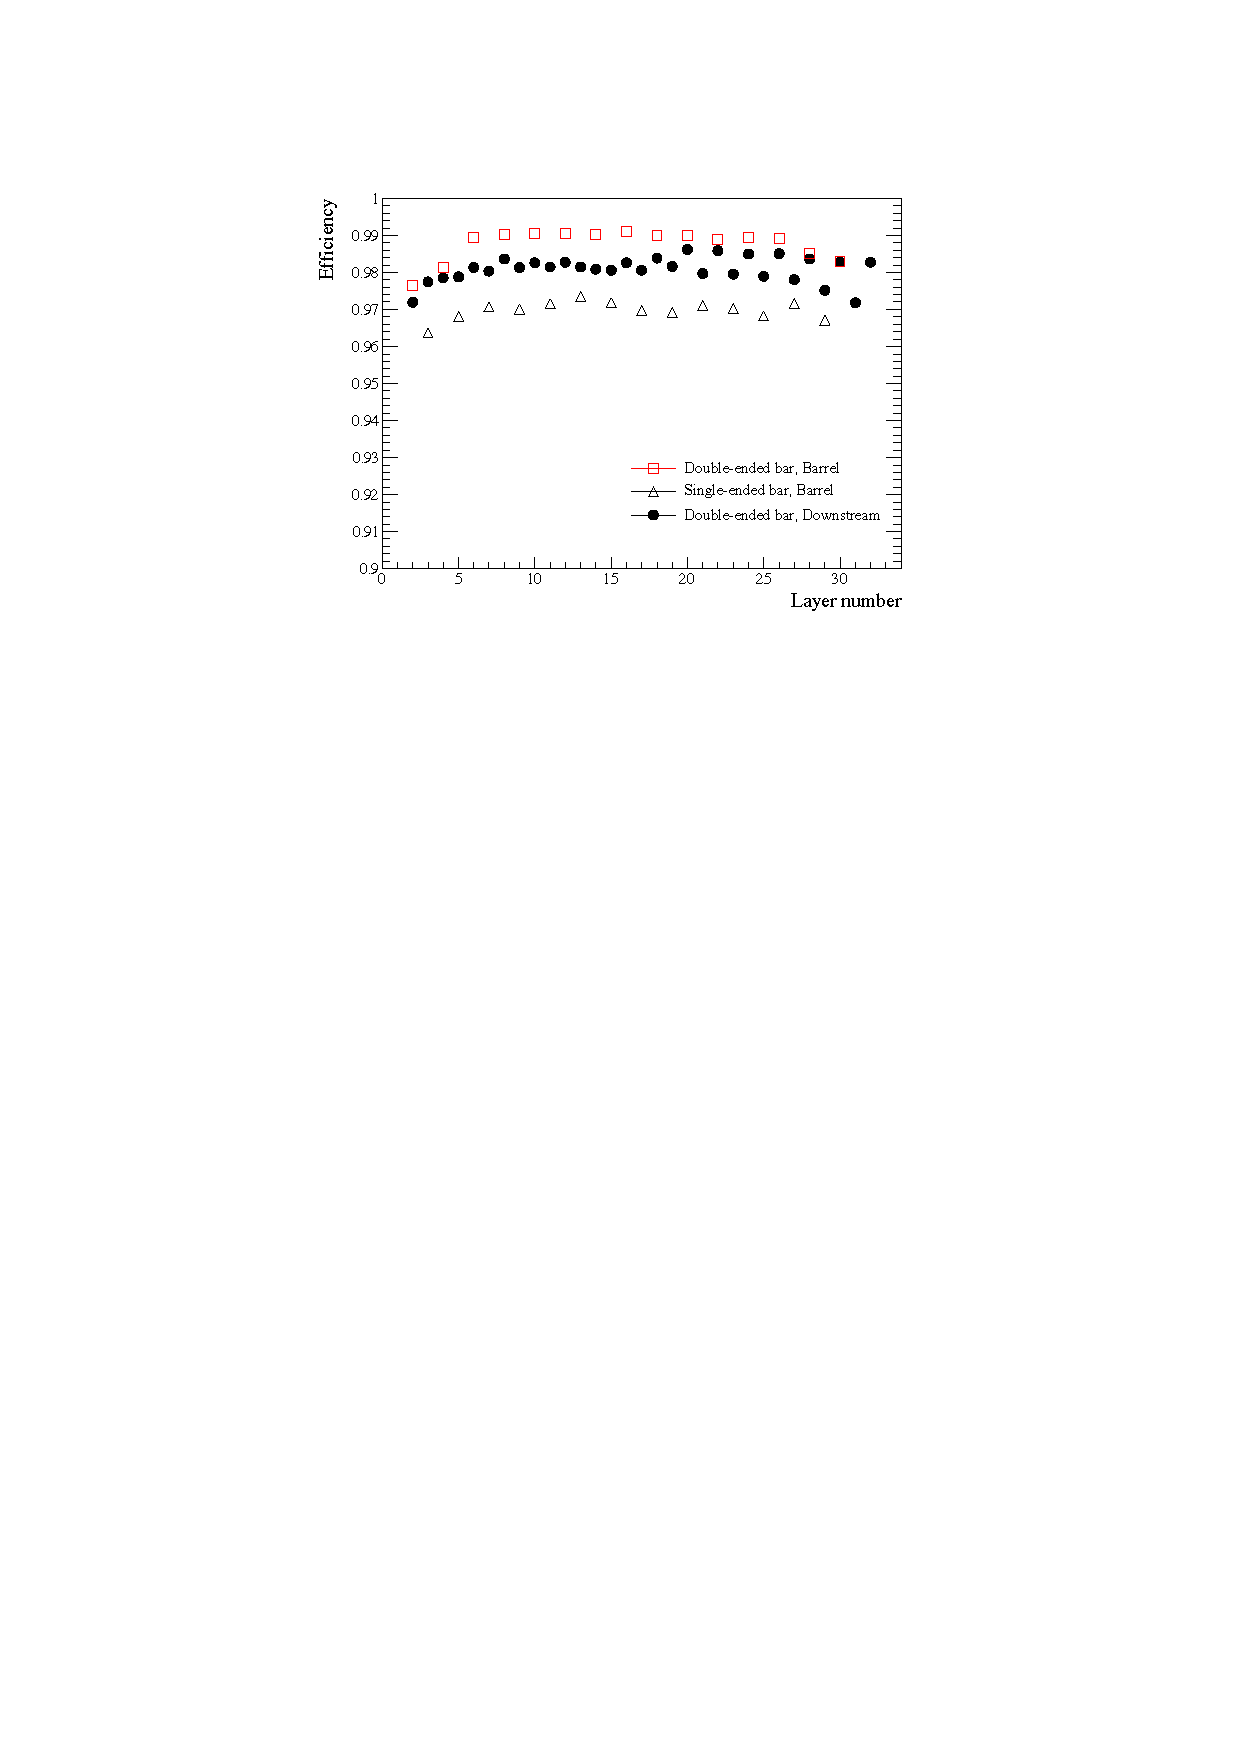
\includegraphics[width=10cm]{images/measurement/systematics/detector/threshold/layer_efficiency_cosmics_data.pdf}
  \caption{The layer-by-layer efficiency for the ND280 ECals, measured using cosmic data~\cite{1748-0221-8-10-P10019}.}
  \label{fig:LayerEfficiencyCosmicData}
\end{figure}
\begin{itemize}
\item The MC hit efficiency is 100$\%$.
\item The data hit efficiency for all bars is the lowest efficiency shown in Fig.~\ref{fig:LayerEfficiencyCosmicData}, which is 96.2$\%$.
\end{itemize}
Bearing the assumptions in mind, the hit inefficiency which must be applied to the MC is 3.8$\%$.  Care must be taken when attempting to apply the hit inefficiency to the MC.  Naively, one might attempt to randomly remove 3.8$\%$ of hits from the reconstruction\Yoshi{; however,}{ADDRESSED - was ``, however''} this would not best represent the hit inefficiency.  There are many reasons why a scintillator bar would not be $100\%$ efficient\Yoshi{; however,}{ADDRESSED - was ``, however''} the efficiency should correlate with the deposited charge.  So, to best model this systematic effect, the lowest 3.8$\%$ of hits should be removed from the MIP peak in charge space.  Fig.~\ref{fig:HitChargeCosmicMCPEU} shows the deposited charge for each hit created by MC cosmic rays.
\begin{figure}[b!]
  \centering
  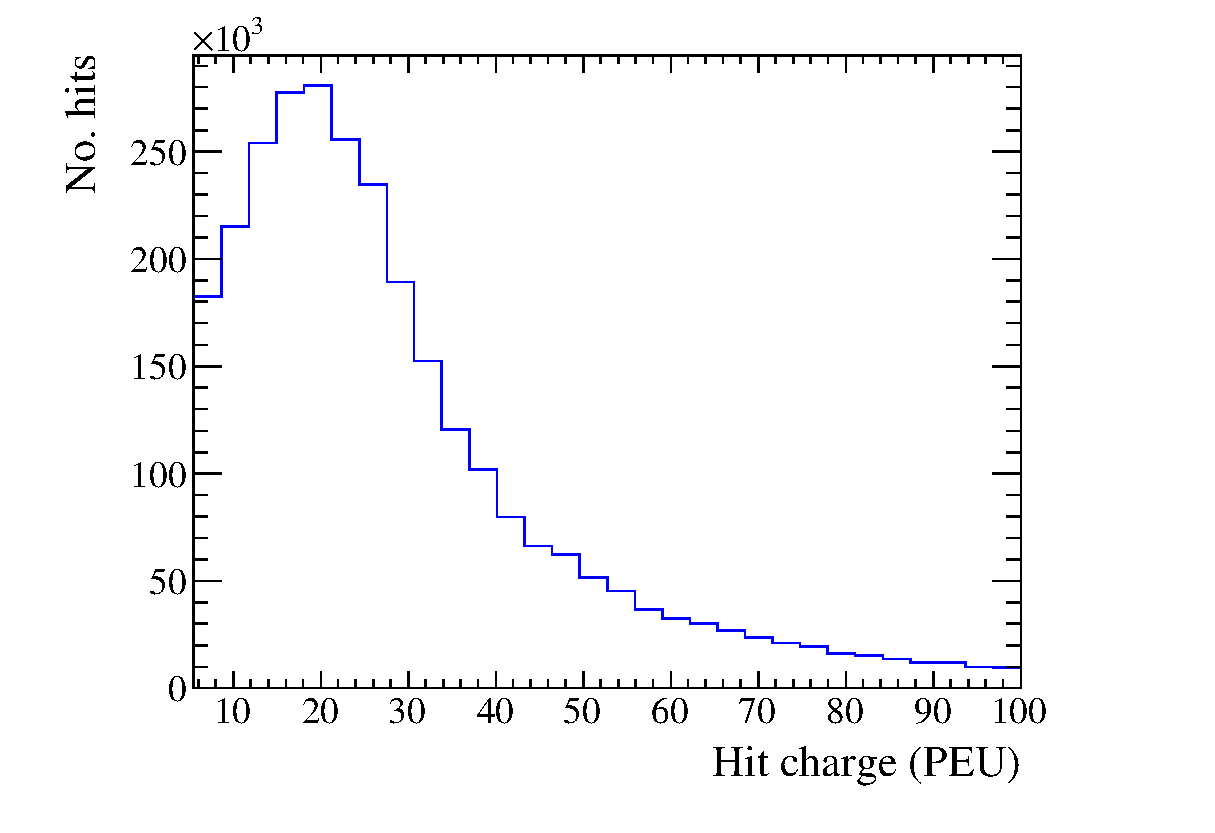
\includegraphics[width=10cm]{images/measurement/systematics/detector/threshold/hit_charge_cosmic_MC_PEU.eps}
  \caption{The charge distribution of scintillator bar hits created by MC cosmic rays.}
  \label{fig:HitChargeCosmicMCPEU}
\end{figure}
The distribution is cut off at 5.5 PEU as this is a minimum threshold for output hits in the calibration stage of the ND280 software.  The clearly visible MIP peak is very close to this threshold and is actually partially cut off by this limit.  So, to apply the hit inefficiency, a new threshold needs to be calculated which removes an extra 3.8$\%$ of the lowest charge hits.  By applying this logic to the hits used in Fig~\ref{fig:HitChargeCosmicMCPEU}, the new threshold was calculated to be 7.55~PEU.  This new threshold was applied as an initial stage of the reconstruction.  The reconstruction and selection was then reapplied to the sample.  This new sample was then compared to the nominal sample to construct the covariance matrices, which are shown in Fig.~\ref{fig:ECalThresholdCovarianceMatrices}.  The largest uncertainty for the samples was found to be 3.74$\%$.
\begin{figure}%
  \centering
  \subfloat[Shape+normalisation.]{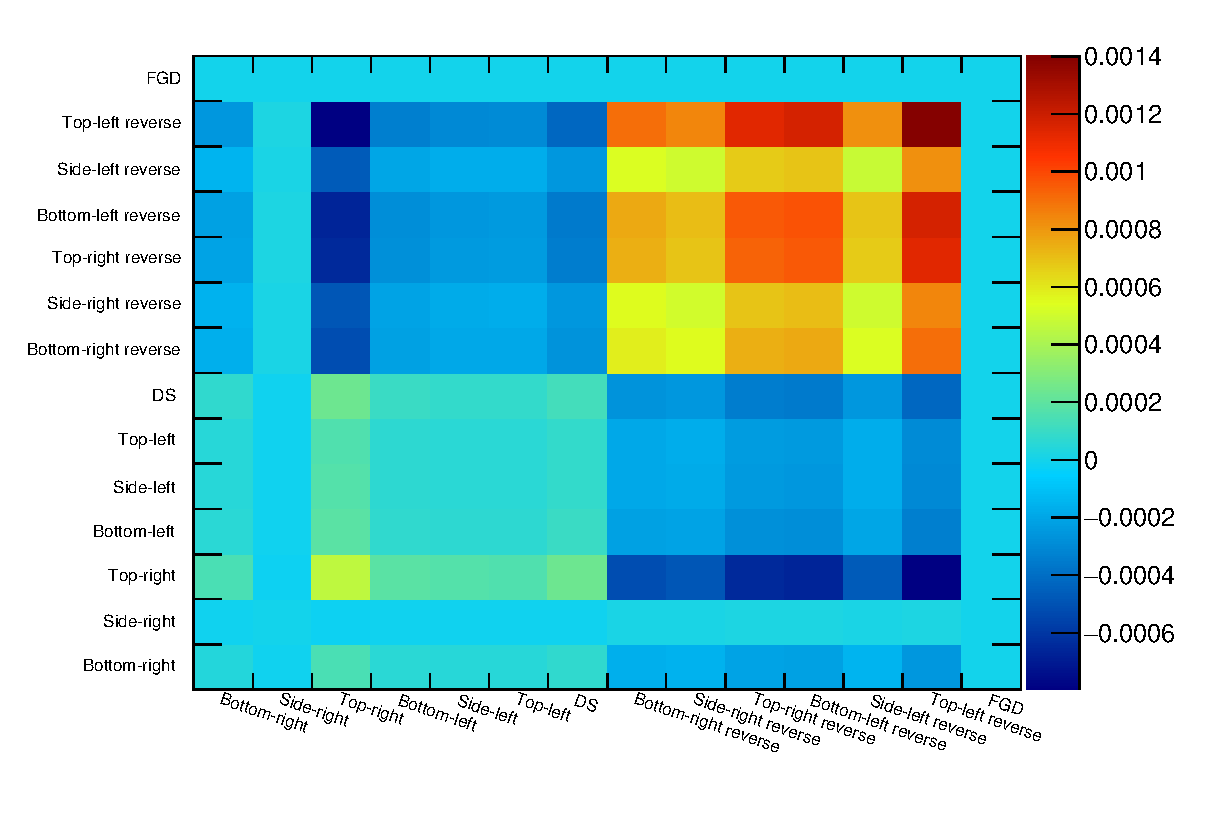
\includegraphics[width=8cm]{images/measurement/systematics/detector/threshold/ecal_threshold_covariance_matrix.eps} \label{fig:ECalThresholdShapeNormCovarianceMatrix}}
  \subfloat[Shape-only.]{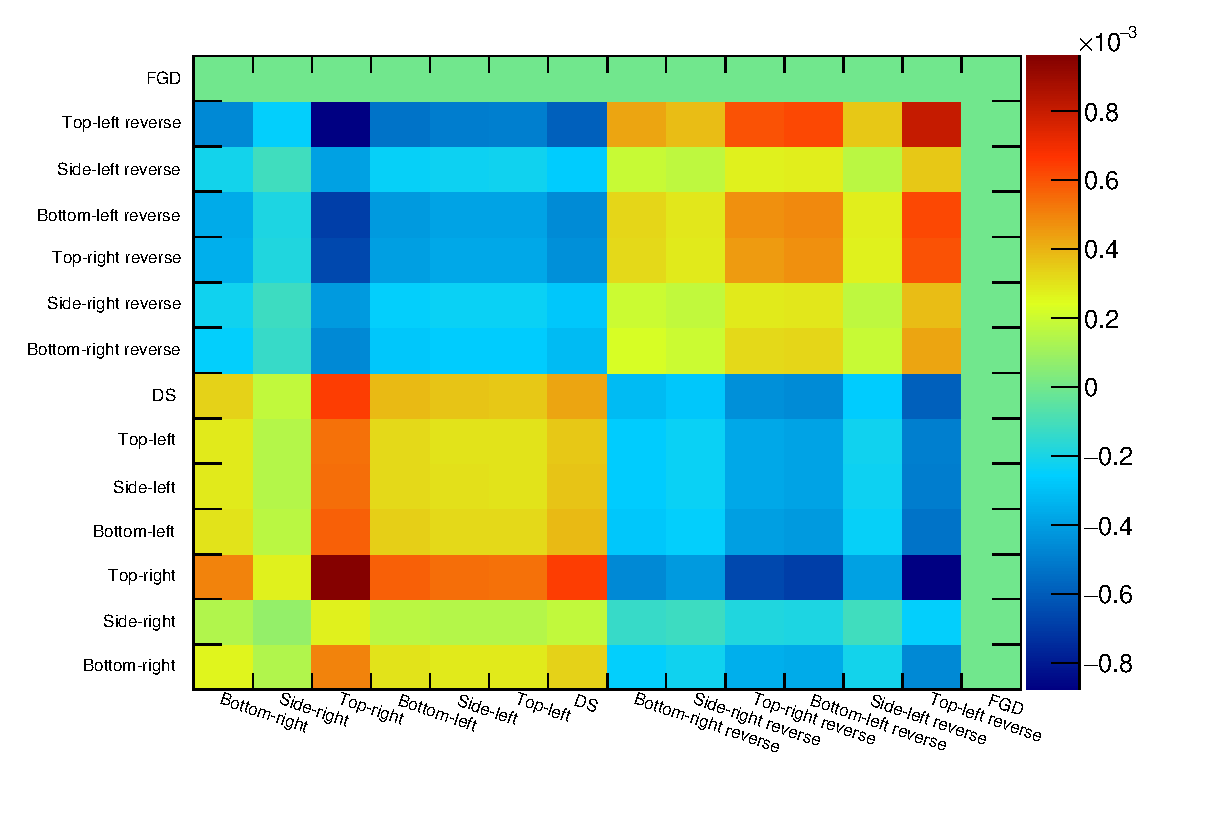
\includegraphics[width=8cm]{images/measurement/systematics/detector/threshold/ecal_threshold_shape_covariance_matrix.eps} \label{fig:ECalThresholdShapeOnlyCovarianceMatrix}}
  \caption{The sample covariance induced by the ECal hit inefficiency.}
  \label{fig:ECalThresholdCovarianceMatrices}
\end{figure}
\newline
\newline
The hit efficiency systematic uncertainty actually covers several areas of uncertainty.  Firstly, it addresses how a change in the core input to the reconstruction changes its output and so, by extension, addresses the efficiency of the reconstruction.  However, because the inefficiency is invoked by removing low charge hits, it also addresses how low charge hits, which could migrate below the minimum reconstruction threshold, could affect the analysis.  Because treatment of the charge by the hit efficiency systematic is partially covered, it is only necessary to additionally address how variation in the charge of the already reconstructed objects could alter the number of objects which pass the selection cuts.  To assess this, a well understood side-band sample is needed such that the hit charge in MC and data can be compared.  Any shift or smearing of the charge in data, relative to Monte Carlo must then be added to the reconstructed objects, which can then be passed through the selection, allowing the covariance matrices to be constructed.  To study the variation in the hit charge, a sample of cosmic MC and data was used.  The two samples were passed through the enhanced reconstruction and the charge of the hits associated to the reconstructed events were then analysed.  An example of the reconstructed hit charges is shown in Fig.~\ref{fig:HitChargeNominalCosmicsTLB}.  
\begin{figure}%
  \centering
  \subfloat[Data and nominal MC.]{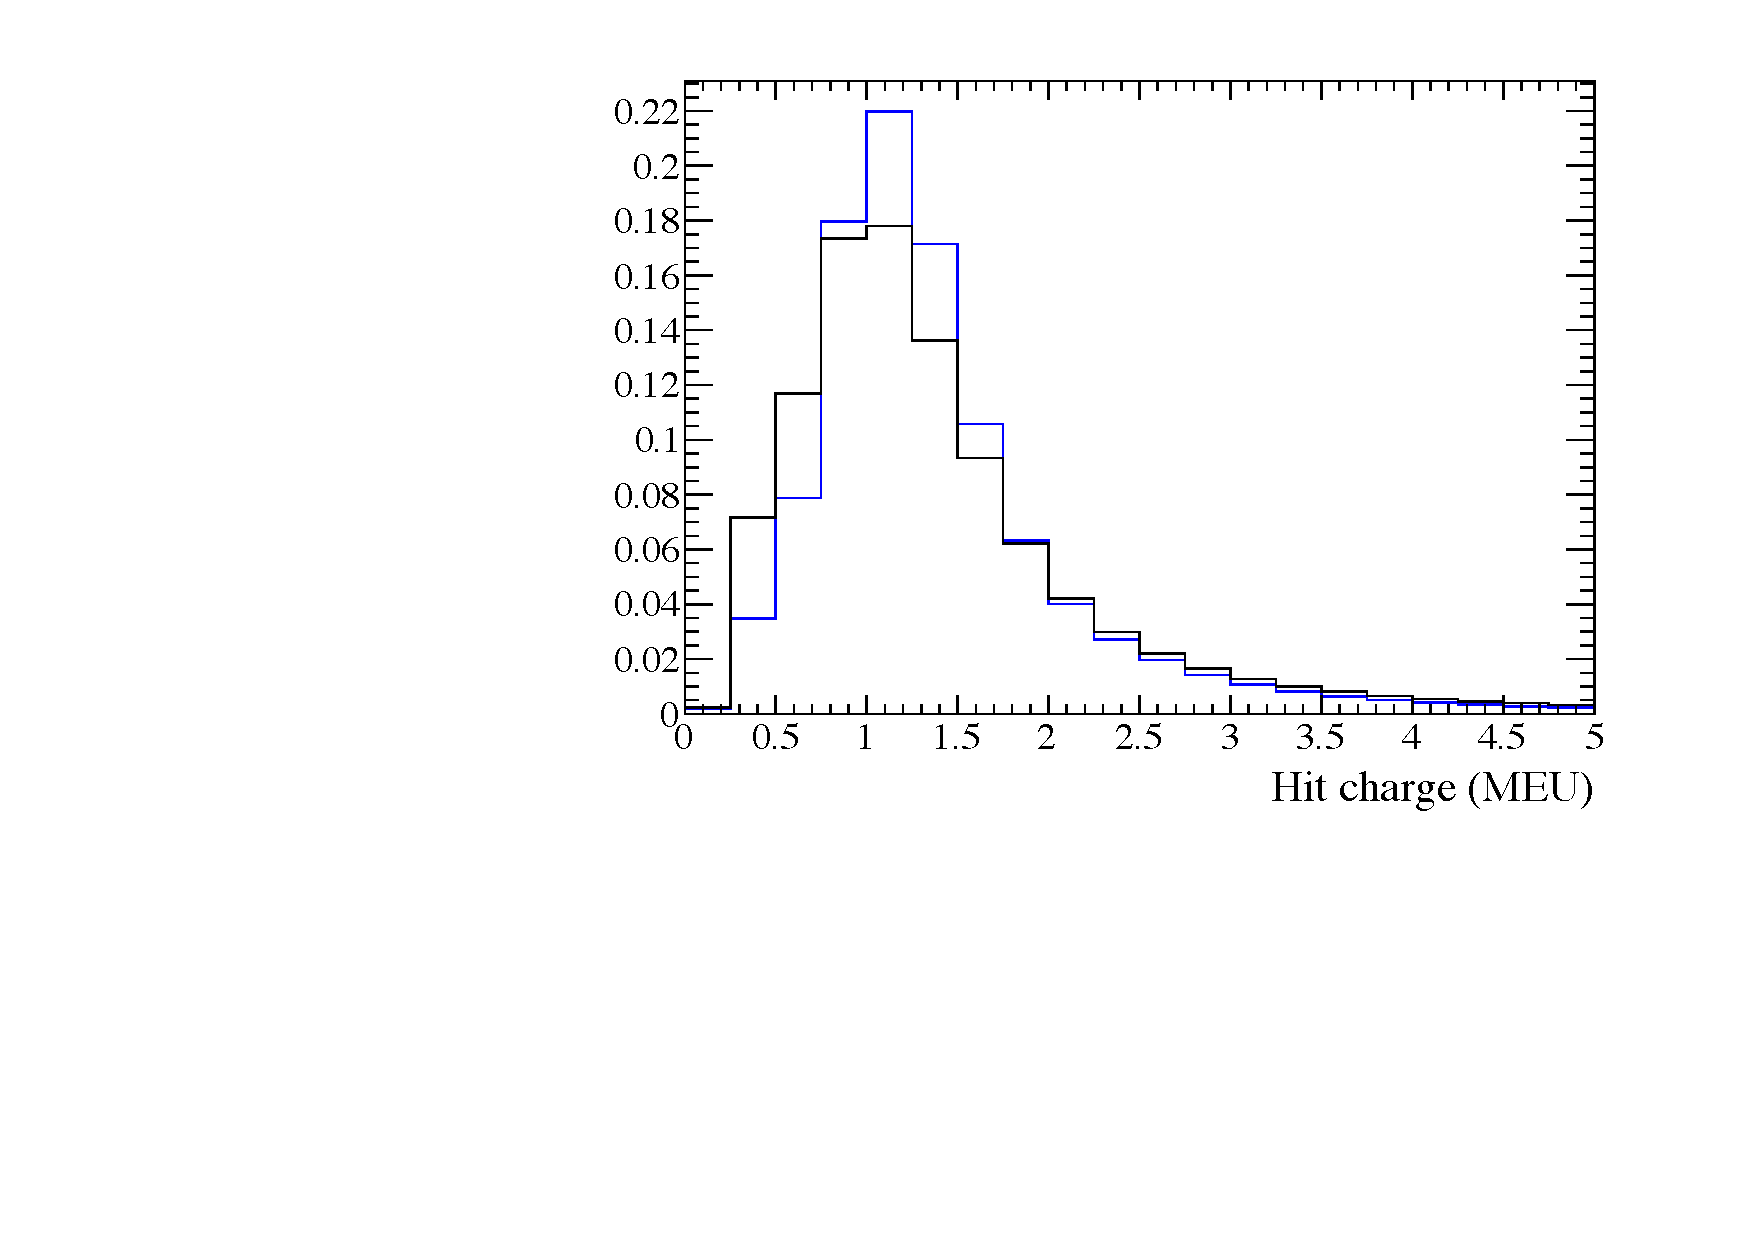
\includegraphics[width=8cm]{images/measurement/systematics/detector/charge/HitCharge_Cosmics_TLB.pdf} \label{fig:HitChargeNominalCosmicsTLB}}
  \subfloat[Data and shifted+smeared MC.]{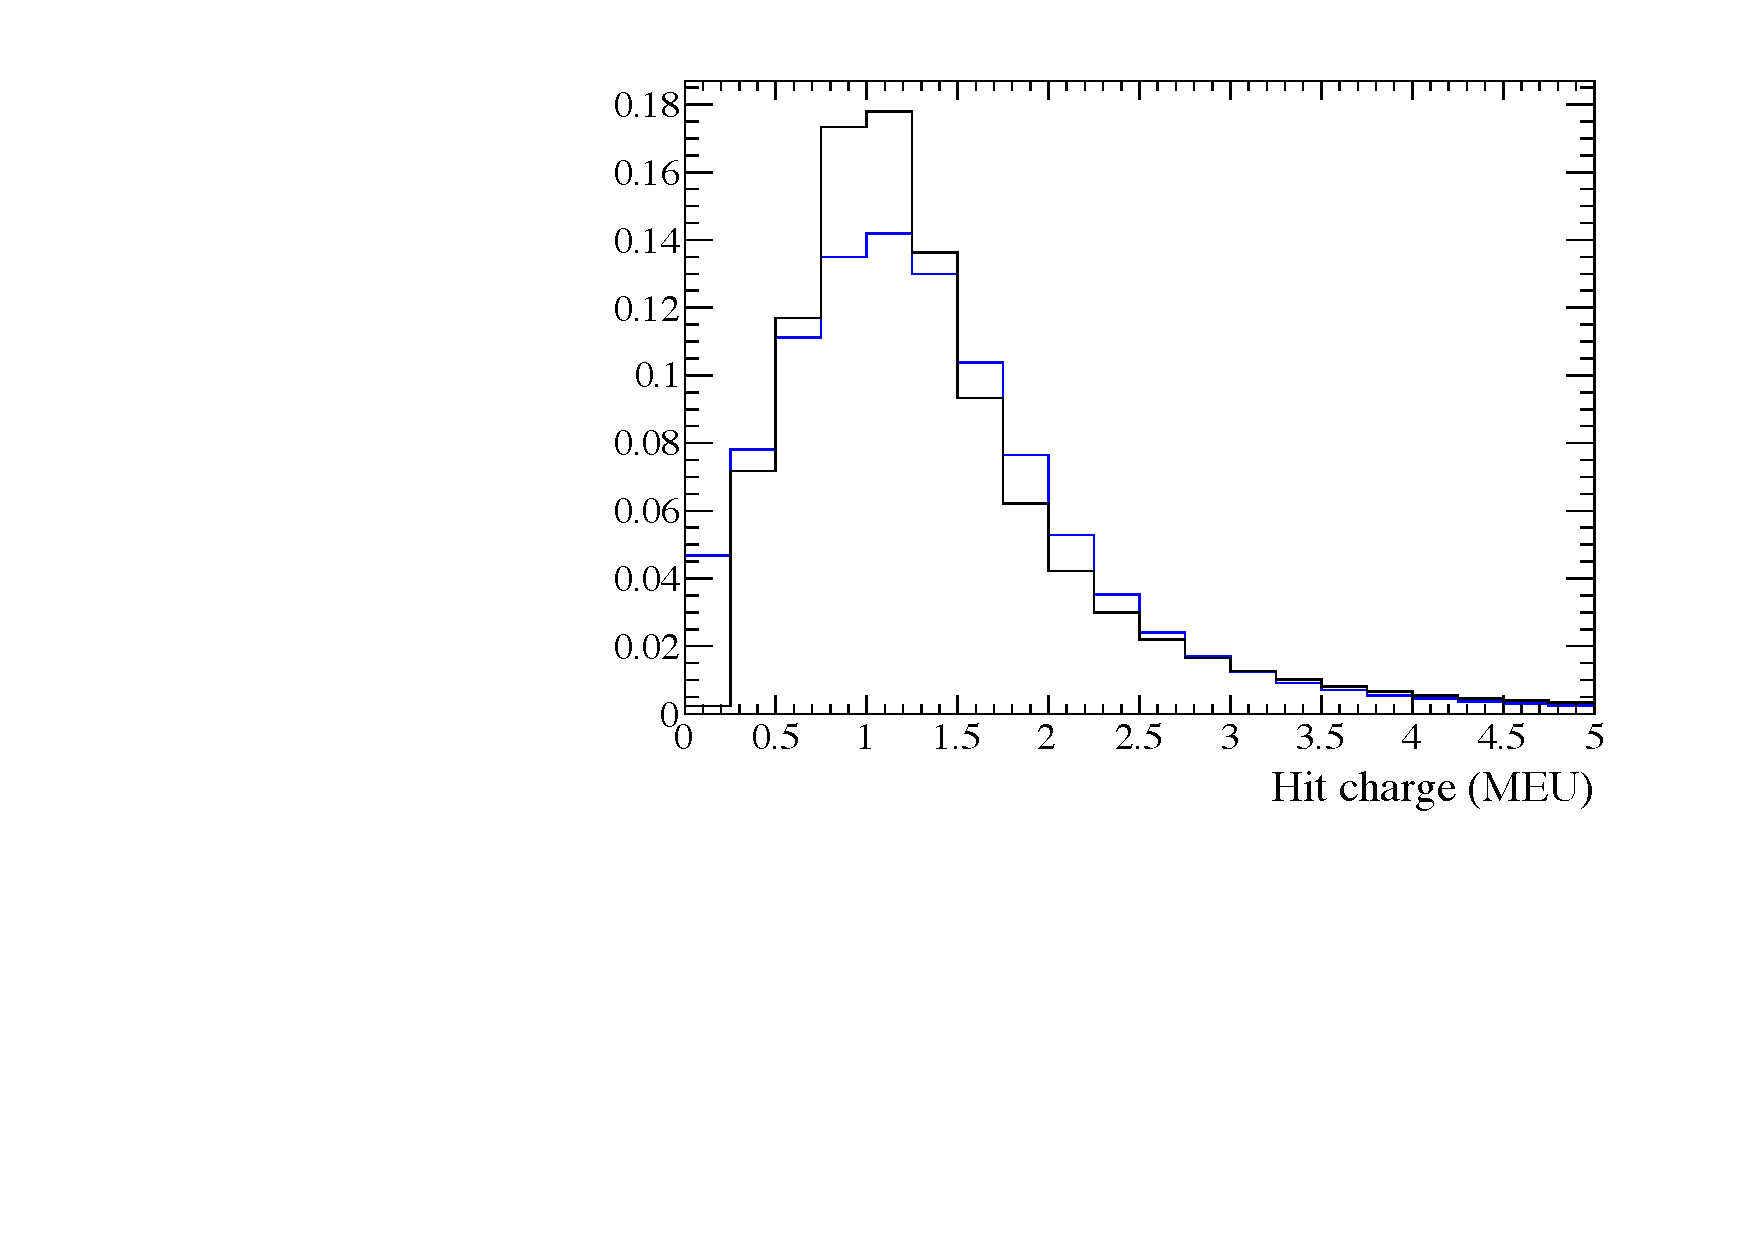
\includegraphics[width=8cm]{images/measurement/systematics/detector/charge/HitChargeCorrected_Cosmics_TLB.pdf} \label{fig:HitChargeCorrectedCosmicsTLB}}
  \caption{The charge of ECal hits after applying the enhanced reconstruction to run 3C cosmic events.  The distributions only show information for reconstructed objects in the top-left barrel ECal module.  The blue and black histograms are Monte Carlo and data respectively.}
  \label{fig:ECalThresholdCovarianceMatrices}
\end{figure}
There are clear differences in the shape of the two distributions; the data charge peak is wider than the MC peak.  To quantify this difference in the peak of the distributions, a Gaussian was fit to the top 66$\%$ of the two peaks which were then compared.  The relevant parameters for the comparison are the width of the data and MC fits, $\sigma_{\textrm{Data}}^{Q}$ and $\sigma_{\textrm{MC}}^{Q}$ respectively, and 
\begin{equation}
\Delta^Q = \mu_{\textrm{Data}}^Q - \mu_{\textrm{MC}}^Q,
\end{equation}
where $\mu_{\textrm{Data}}^Q$ and $\mu_{\textrm{MC}}^Q$ are the mean of the data and MC fits respectively.  $\Delta^Q$ measures the shift of the MC peak relative to data, while $\sigma_{\textrm{Data}}^{Q}$ and $\sigma_{\textrm{MC}}^{Q}$ can be used to quantify the relative width.  These values are shown in table~\ref{table:HitChargeFitValues}.  To truly quantify the difference in the charge distributions, not only is a well understood sample required, but also a clean set of reconstructed events to remove any additional effects which may mask the charge difference.  As the cosmic events will generally be almost parallel to the vertical axis, only the top and bottom ECal modules will be able to cleanly reconstruct the cosmic events, so only those events should be considered.  Ideally, the values shown in table~\ref{table:HitChargeFitValues}, would be used to correct and smear the MC peak to match data.  
\begin{table}
  \begin{tabular}{ c c c c }
   ECal module & $\Delta^{Q}$ (MEU) & $\sigma_{\textrm{Data}}^Q$ (MEU) & $\sigma_{\textrm{MC}}^Q$ (MEU) \\ \hline \hline
   Bottom-right & -0.095 & 0.37 & 0.51 \\
   Bottom-left & +0.045 & 0.37 & 0.61 \\
   Top-right & -0.003 & 0.38 & 0.58 \\
   Top-left & -0.099 & 0.38 & 0.50 \\ \hline
   Side-right & -0.225 & 0.83 & 0.64 \\
   Side-left & -0.315 & 0.85 & 0.55 \\
   DS & -0.472 & 0.87 & 0.46 \\
  \end{tabular}
  \caption{Summary of the lead absorbers for the ND280 Tracker ECals~\cite{1748-0221-8-10-P10019}.}
  \label{table:HitChargeFitValues}
\end{table}
However, due to time constraints, it was only possible to use said values to over-correct and over-smear the MC.  In terms of the individual hits, this meant using $\Delta^{Q}$ and $\sigma_{\textrm{Data}}^Q$ for the top-left ECal to apply a correction and smearing to the hit charges, regardless of which module the hit occurred in.  The top-left ECal module was chosen because it  has the largest value of $\Delta^{Q}$.  The adjusted hit charge is
\begin{equation}
Q' = Q + X
\label{eqn:HitChargeCorrection}
\end{equation}
where $Q$ is the nominal hit charge and $X$ is a random variable which is defined as 
\begin{equation}
X \sim N(\Delta^{Q},\sigma_{\textrm{Data}}^Q).
\label{eqn:HitChargeRandomVariable}
\end{equation}
It is important to note here that the width of the Gaussian distribution in which the adjustment is drawn from is $\sigma_{\textrm{Data}}^Q$.  By using this width, the MC hit charge is over-smeared relative to data.  An example application of equation~\ref{eqn:HitChargeCorrection} is shown in Fig.~\ref{fig:HitChargeCorrectedCosmicsTLB} which uses the same hit information as that in Fig.~\ref{fig:HitChargeNominalCosmicsTLB}, but with the correction applied to the MC hit charge.  As can be seen by comparing the two figures, the application of the over-smearing has caused the MC charge peak to be wider than the data peak.  To propagate the effect of this systematic, this smearing and correction needs to be applied to the reconstructed prongs before any selection takes place.  Unfortunately, hit level information is not available at the level where the selection is applied.  So, a slightly modified charge adjustment is needed.  If the total charge contained on a prong is $Q_{\textrm{prong}}$, then the total adjusted charge is
\begin{equation}
Q'_{\textrm{prong}} = Q_{\textrm{prong}} + X_{\textrm{prong}}
\label{eqn:ProngChargeRandomVariable}
\end{equation}
where $X_{\textrm{prong}}$ is a random variable and is defined as
\begin{equation}
X \sim N(\Delta^{Q}N_{\textrm{prong}},\sigma_{\textrm{Data}}^Q),
\label{eqn:HitChargeRandomVariable}
\end{equation}
where $N_{\textrm{prong}}$ is the number of hits contained on the prong.  Following the above description, the prong charge variation was applied to every reconstructed prong in the systematic sample and the selection was then applied.  This process was repeated 1000 times to build up the covariance matrices, which are shown in Fig.~\ref{fig:ECalChargeCovarianceMatrices}.
\begin{figure}%
  \centering
  \subfloat[Shape+normalisation.]{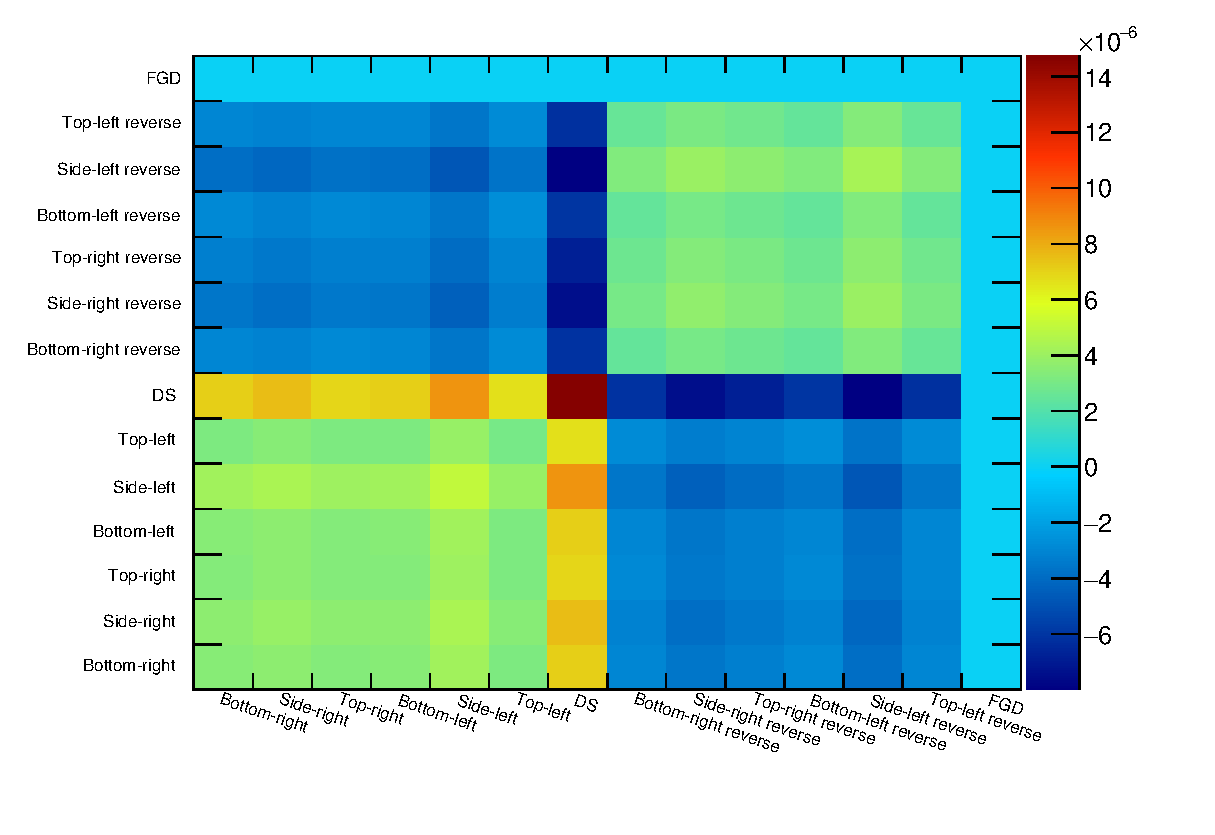
\includegraphics[width=8cm]{images/measurement/systematics/detector/charge/ecal_charge_covariance_matrix.eps} \label{fig:ECalChargeShapeNormCovarianceMatrix}}
  \subfloat[Shape-only.]{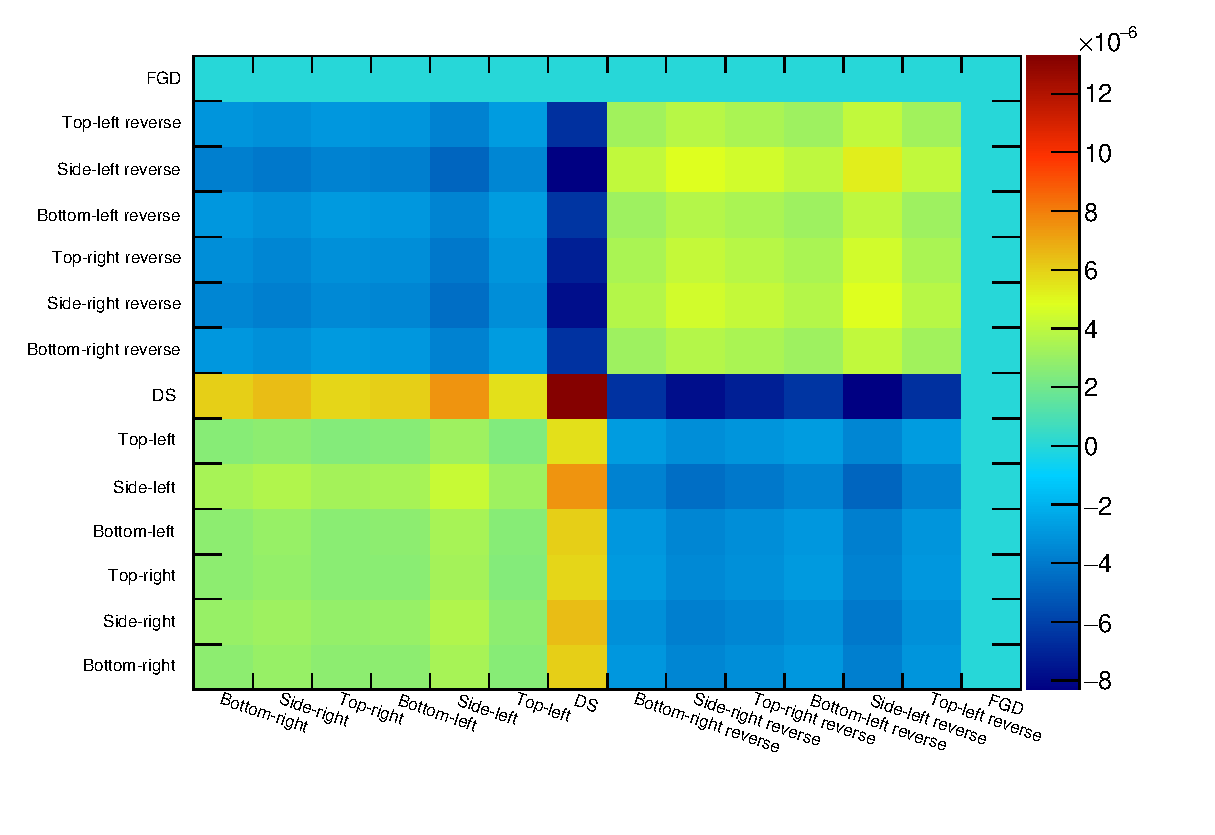
\includegraphics[width=8cm]{images/measurement/systematics/detector/charge/ecal_charge_shape_covariance_matrix.eps} \label{fig:ECalChargeShapeOnlyCovarianceMatrix}}
  \caption{The sample covariance induced by the ECal charge uncertainties.}
  \label{fig:ECalChargeCovarianceMatrices}
\end{figure}
\newline
\newline
While the hit efficiency and charge systematic assessments are fairly all-encompassing in terms of ECal detector uncertainties, they can not address how the inherent noise in the ECal can affect the reconstruction and, by extension, the selected number of events in this analysis.  There is only a need to address a noise systematic uncertainty if the simulated noise rate in the Monte Carlo is different to what actually happens in the ECal.  
\newline
\newline
To measure the noise rate, a control sample  of cosmic rays (for the barrel) and through-going muons (for the DS ECal) were passed through the reconstruction.  Before the clustering stages were initiated, the number of hits in the relevant ECal module were recorded.  Then, after the reconstruction chain was completed, the number of hits which formed the final reconstructed objects were also counted.  The difference between these two numbers forms the noise hit estimate.  To test this estimator, the true number of noise hits in the Monte Carlo were also counted.
\begin{figure}%
  \centering
  \subfloat[Cosmic control sample in the barrel ECals.]{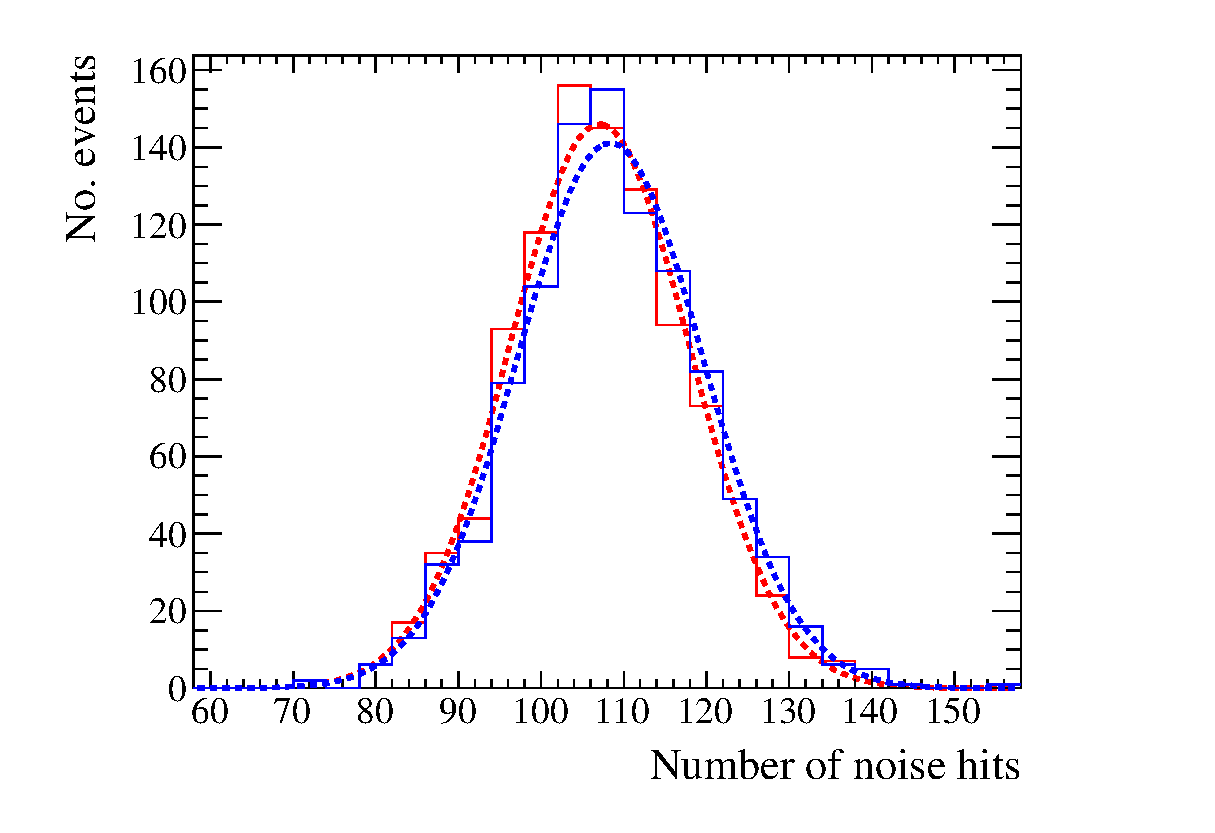
\includegraphics[width=8cm]{images/measurement/systematics/detector/noise/noise_mc_estimate_mc_true_barrel.eps} \label{fig:ECalNoiseMCEstimateMCTrueBarrel}}
  \subfloat[Through-going muon control sample in the DS ECal.]{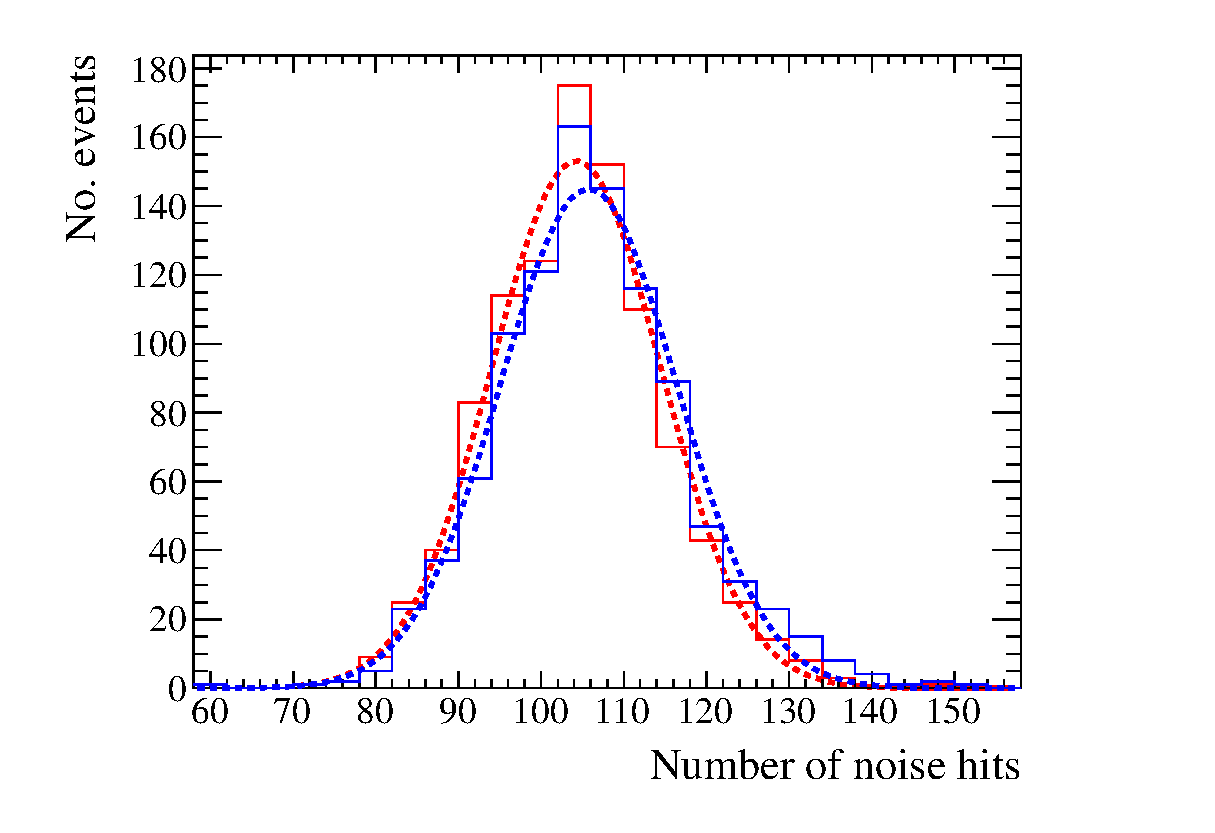
\includegraphics[width=8cm]{images/measurement/systematics/detector/noise/noise_mc_estimate_mc_true_ds.eps} \label{fig:ECalNoiseMCEstimateMCTrueDS}}
  \caption{The estimation of the number of noise hits (solid blue line) and the number of true noise hits (solid red line) per event in Monte Carlo.  The coloured dashed lines are the Gaussian fits to the respective distributions.}
  \label{fig:ECalNoiseMCEstimateMCTrue}
\end{figure}
The results of this test are shown in Fig.~\ref{fig:ECalNoiseMCEstimateMCTrue}.  The Gaussian fits to the distribution are used to quantify the noise levels per event (by using the mean and width of the fits).  These values are shown in table~\ref{table:NoiseRateSummary}.  The estimate is clearly in good agreement with the true noise levels in the Monte Carlo.  So, it was decided to apply this method to estimate the noise levels in the data samples, the results of which are shown in Fig.~\ref{fig:ECalNoiseMCEstimateDataEstimate} and also shown in table~\ref{table:NoiseRateSummary}.
\begin{figure}%
  \centering
  \subfloat[Cosmic control sample in the barrel ECals.]{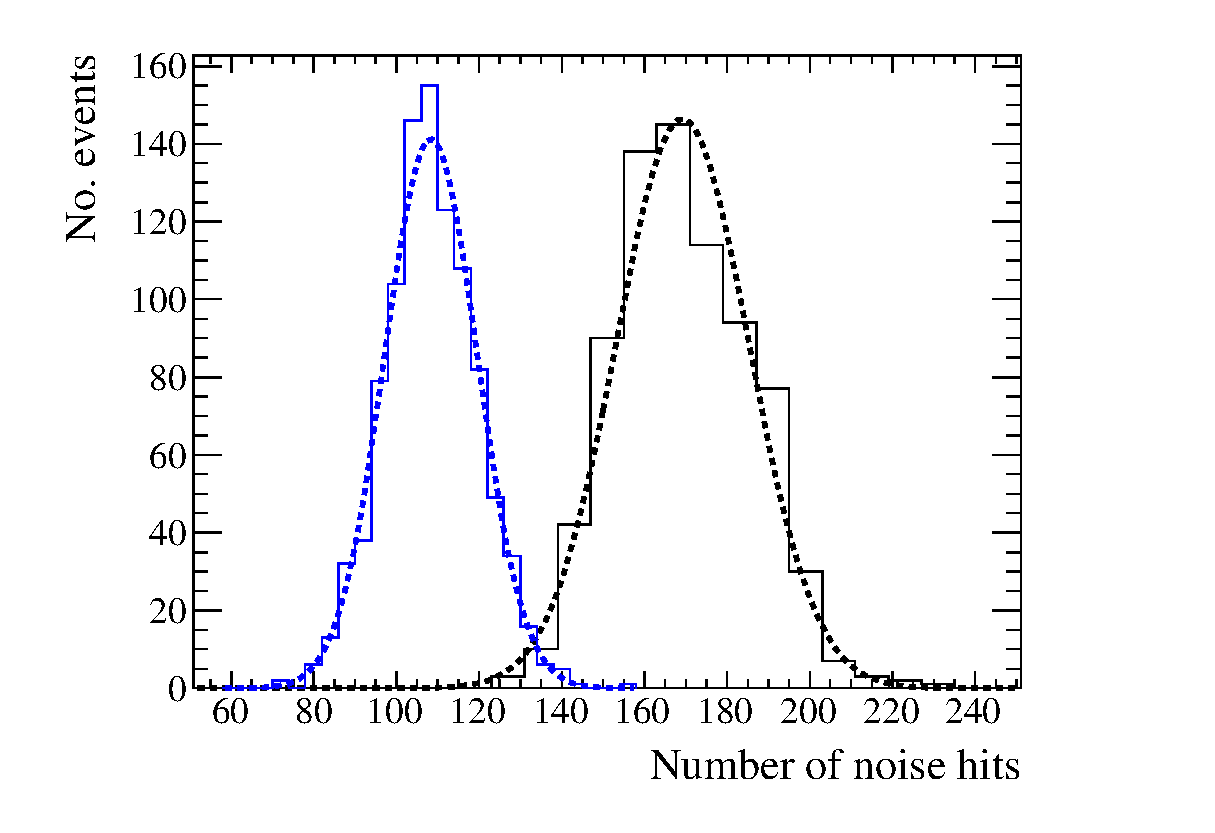
\includegraphics[width=8cm]{images/measurement/systematics/detector/noise/noise_mc_estimate_data_estimate_barrel.eps} \label{fig:ECalNoiseMCEstimateDataEstimateBarrel}}
  \subfloat[Through-going muon control sample in the DS ECal.]{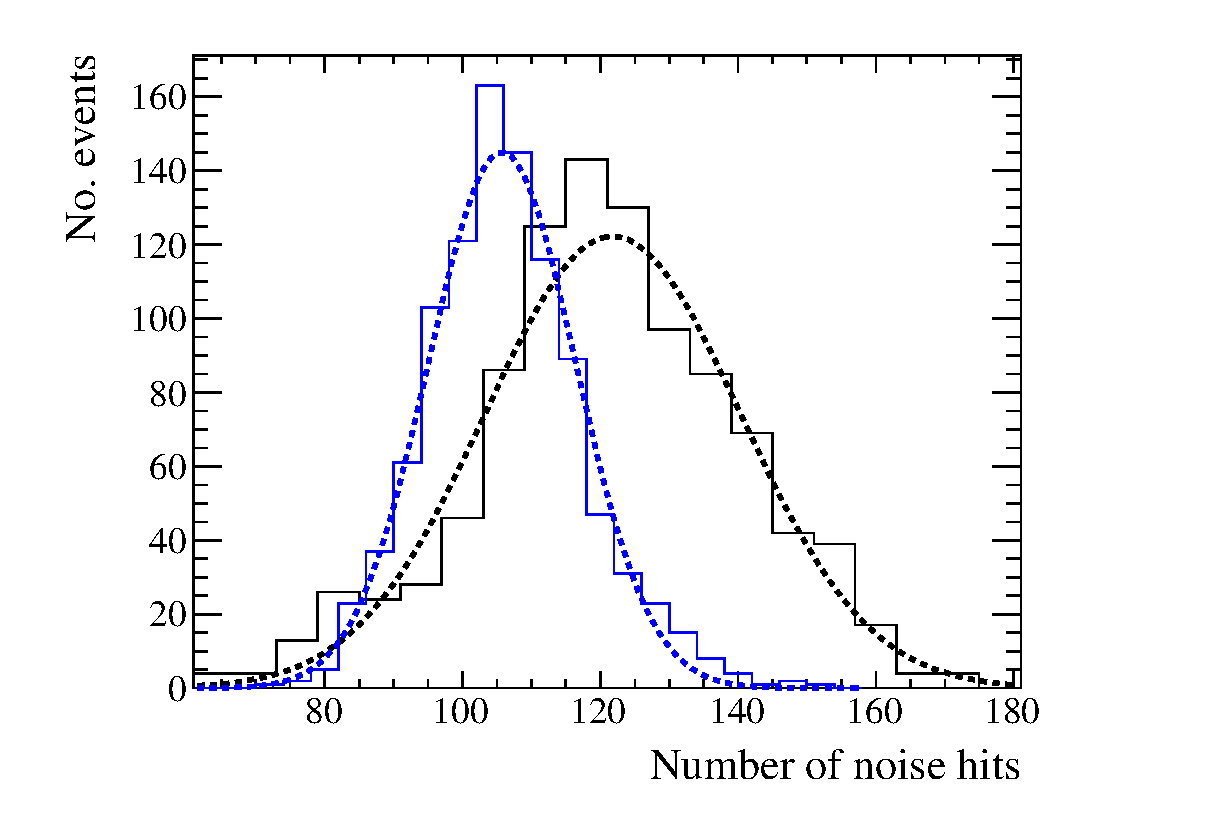
\includegraphics[width=8cm]{images/measurement/systematics/detector/noise/noise_mc_estimate_data_estimate_ds.eps} \label{fig:ECalNoiseMCEstimateDataEstimateDS}}
  \caption{The estimation of the number of noise hits in Monte Carlo (solid blue line) and data (solid black line) per event.  The coloured dashed lines are the Gaussian fits to the respective distributions.}
  \label{fig:ECalNoiseMCEstimateDataEstimate}
\end{figure}
\begin{table}
  \begin{tabular}{ c c c c}
  ECal module(s) & True (MC) & Estimated (MC) & Estimated (data)  \\ \hline \hline
  Barrel & $107\pm10$ & $108\pm11$ & $169\pm16$ \\
  DS & $104\pm10$ & $106\pm11$ & $122\pm18$ \\
  \end{tabular}
  \caption{Summary of the study to estimate the number of noise hits per event in the ECals.}
  \label{table:NoiseRateSummary}
\end{table}
It is clear that there are differences between the noise levels in data and Monte Carlo.  So, to propagate the effect of this systematic uncertainty, elecSim was retuned to produce the data-like noise levels in both the barrel and DS ECal.  The systematic sample was then passed through the modified elecSim and all pieces of the software chain downstream.  After this, the selection was applied to the modified sample.  This sample was then compared to nominal and the difference was used to construct the covariance matrices, which are shown in Fig.~\ref{fig:ECalNoiseCovarianceMatrices}.
\begin{figure}%
  \centering
  \subfloat[Shape+normalisation.]{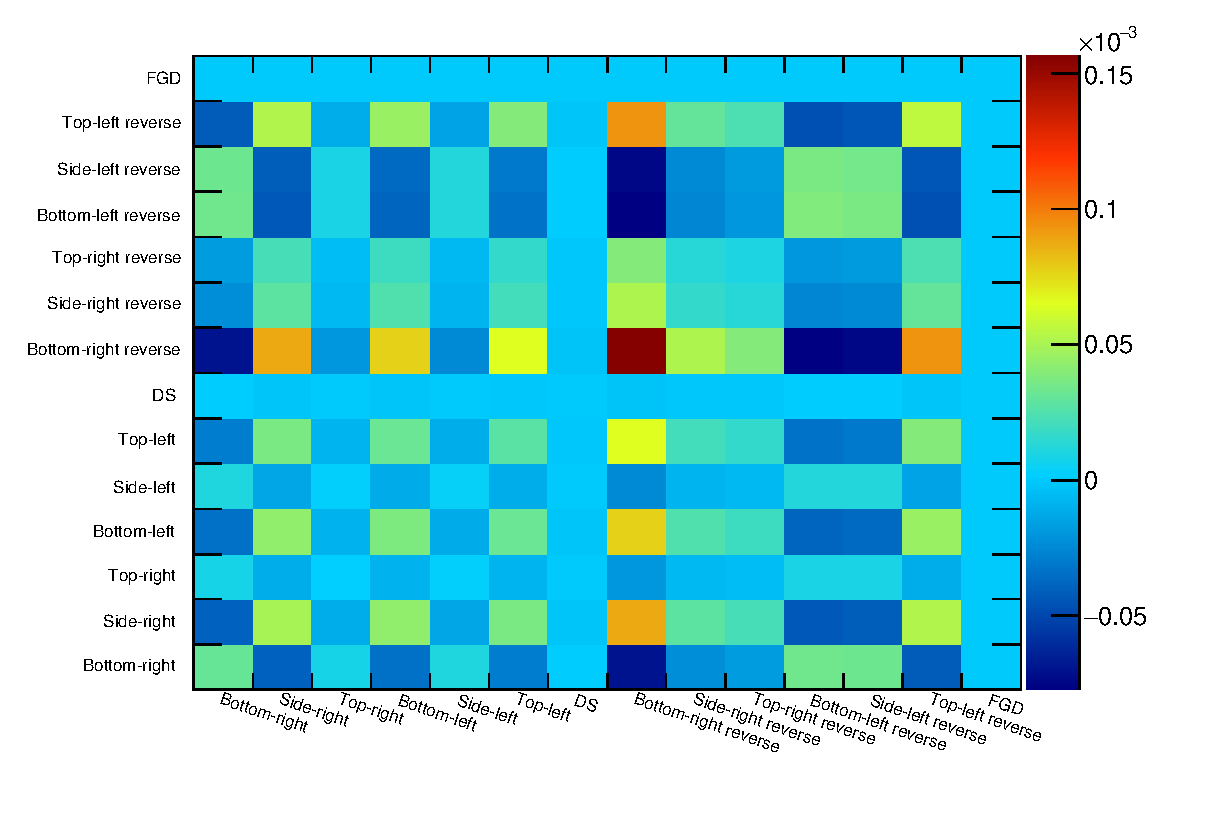
\includegraphics[width=8cm]{images/measurement/systematics/detector/noise/ecal_noise_covariance_matrix.eps} \label{fig:ECalNoiseShapeNormCovarianceMatrix}}
  \subfloat[Shape-only.]{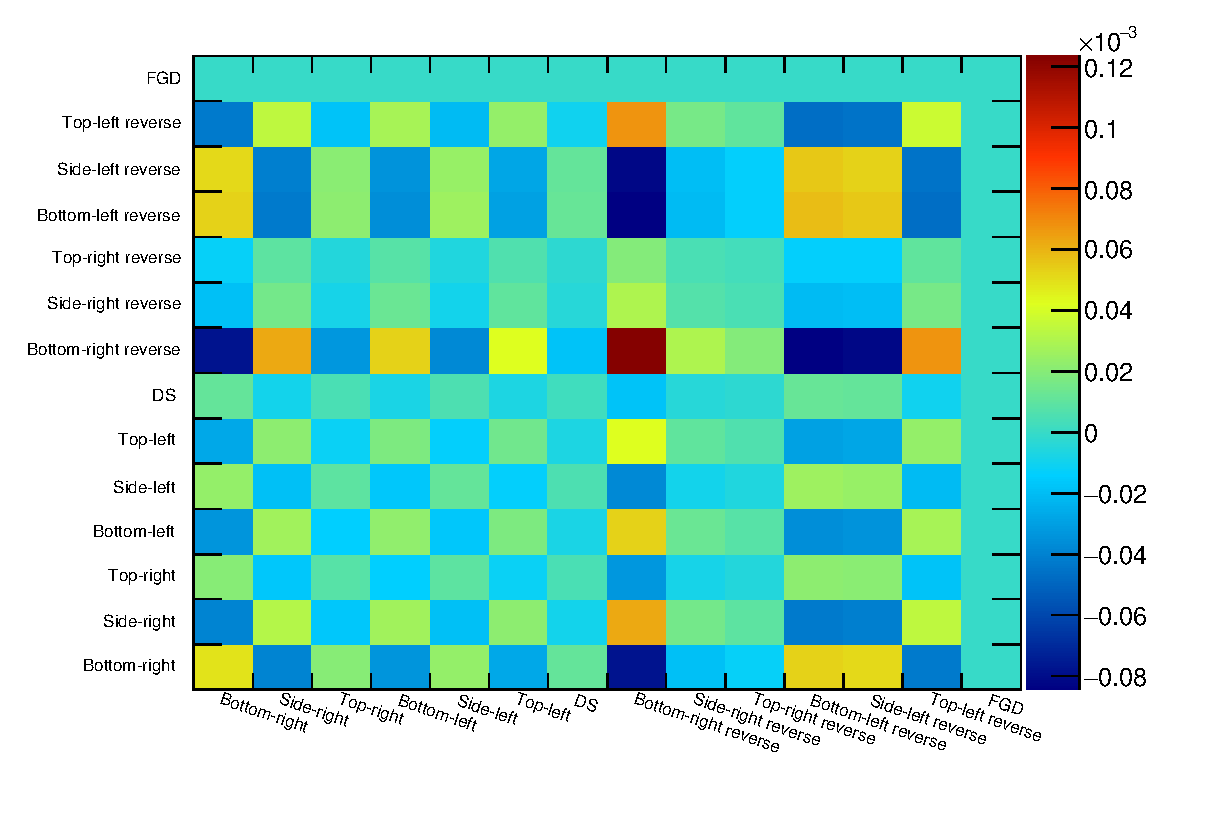
\includegraphics[width=8cm]{images/measurement/systematics/detector/noise/ecal_noise_shape_covariance_matrix.eps} \label{fig:ECalNoiseShapeOnlyCovarianceMatrix}}
  \caption{The sample covariance induced by the ECal noise uncertainties.}
  \label{fig:ECalNoiseCovarianceMatrices}
\end{figure}
\newline
\newline
The ECal model used in the simulation was based on the as built drawings and so should be an accurate model.  However, the components of each ECal module do have associated uncertainties which are not, and can not easily be, taken into account in the simulation, but could easily cause a systematic difference between data and Monte Carlo.  For example, if the DS ECal lead absorbers were thicker in the simulated model, one should expect to see a relative deficit of beam triggered events in the DS ECal collected data.  Provided that the component dimensions, compositions and uncertainties are known, toy Monte Carlo can be used to construct a set of toy ECal modules which model the variation in the module mass.  This can be expanded further, to construct a covariance matrix for the total mass of each contributing element.  This covariance matrix can then be used to re-weight the events, based on target element, in the Monte Carlo sample to model the effect of the ECal mass systematic.  
\newline
\newline
The ECal module designs are split into three types: side, top/bottom and DS.  It is only necessary to generate a mass covariance matrix for each of the three types.  All values used for the component dimensions/uncertainties are taken from~\cite{1748-0221-8-10-P10019}.  Precise component dimensions are only quoted for the components in the active regions of each module, namely the lead absorbers, the scintillator bars and the wavelength-shifting fibres.  So, only these components are considered in the toy Monte Carlo study.  
%A summary of the components are shown in table~\ref{table:SideECalComponents}, table~\ref{table:TopBottomECalComponents} and table~\ref{table:DSECalComponents} for the side, top/bottom and DS ECal designs respectively.
\begin{table}[t!]
  \begin{tabular}{ c c c c }
     & Top/Bottom & Side & DS \\ \hline \hline
  No. per layer & 2 & 4 & 2 \\
  Length (mm) & $3858\pm4$ & $964.5\pm4$ & $2016\pm1$ \\
  Width (mm) & $765\pm4$ & $2330\pm4$ & $1008\pm4$ \\
  Height (mm) & $1.75\pm0.1$ & $1.75\pm0.1$ & $1.75\pm0.1$ \\
  Sb doping & $2.0\pm0.2\%$ & $2.0\pm0.2\%$ & $2.0\pm0.2\%$ \\
  \end{tabular}
  \caption{Summary of the lead absorbers for the ND280 Tracker ECals~\cite{1748-0221-8-10-P10019}.}
  \label{table:LeadAbsorberDimensions}
\end{table}


%The following discusses the construction of the side toy ECal modules.  The choices made and the process followed were the same for all three designs.  
\subsubsection{The lead absorbers}
\label{subsubsec:ECalMassLeadAbsorbers}
Reference~\cite{1748-0221-8-10-P10019} provided a clear description of the composition of the lead absorbers for the ECal module designs, which are summarised in table~\ref{table:LeadAbsorberDimensions}.  All component uncertainties (both dimension and composition) were given as symmetric errors.  To construct an ECal lead layer, each layer dimension was randomly taken from a Gaussian with a mean equal to the quoted dimension and a width equal to the dimension uncertainty.  After the layer volume was defined, the Sb contamination was calculated, also using a Gaussian throw, but using the quoted Sb contamination and its uncertainty as the Gaussian's mean and width.  The described information could then be used to retrieve the mass of the Pb and Sb in an ECal lead layer.

\subsubsection{The scintillator bars}
\label{subsubsec:ECalMassSctintillatorBars}
The information used to construct the toy scintillator bars is summarised in table~\ref{table:ScintillatorBarDimensions}, most of which was found in reference~\cite{1748-0221-8-10-P10019}.  The length of the bars were quoted with symmetric uncertainties (like the lead absorbers), so the length was treated in the same way as the lead absorber dimensions.  The hole and coating dimensions were also treated in the same manner.  However, the width and height were quoted with asymmetric errors and so could not be treated in the same way.  Only a negative uncertainty was quoted, which meant the width and height uncertainties could be treated in a somewhat similar manner, but with random numbers being drawn from a half-Gaussian.  The bar composition was reported as polystyrene doped with $1\%$~PPO (C$_{15}$H$_{11}$NO) and $0.03\%$~POPOP.  For the toy bar construction, the POPOP was considered negligible and so was not included.  The result was that the toy bar composition (excluding the coating) was 99$\%$~CH and 1$\%$~C$_{15}$H$_{11}$NO by mass.  Unfortunately, the full composition of the TiO$_2$ coating was not extensively described.  However, a similar systematic study has already been undertaken for the FGD~\cite{FGDMassTN} which included an investigation of the coating composition.  A representative for the Fermilab facility which extruded the scintillator bars reported that the final composition of the coating was 15$\%$ rutile-form TiO$_2$ and 85$\%$ CH with other contributing compounds considered negligible.  This information was also included in the modelling.  The collected information could then be used to retrieve the contributing mass of each element in a scintillator bar.
\begin{table}[t!]
  \begin{tabular}{ c c c c }
     & Top/Bottom & Side & DS \\ \hline \hline
  No. per layer (para) & 38 & 57 & - \\
  No. per layer (perp) & 96 & 96 & 50 \\
  Length (para) (mm) & $3840\pm0.1$ & $3840\pm0.1$ & - \\
  Length (perp) (mm) & $1520\pm0.1$ & $2280\pm0.1$ & $2000\pm0.1$ \\
  Width (mm) & $40^{+0.0}_{-0.4}$ & $40^{+0.0}_{-0.4}$& $40^{+0.0}_{-0.4}$ \\
  Height (mm) & $10^{+0.0}_{-0.4}$ & $10^{+0.0}_{-0.4}$& $10^{+0.0}_{-0.4}$ \\
  Hole diameter (mm) & $1.75\pm0.1$ & $1.75\pm0.1$ & $1.75\pm0.1$ \\
  Composition (CH:PPO) & 99:1 & 99:1 & 99:1 \\
  Coating thickness (mm) & $0.25\pm0.13$ & $0.25\pm0.13$ & $0.25\pm0.13$ \\
  Coating composition (CH:TiO$_2$) & 85:15 & 85:15 & 85:15 \\
  \end{tabular}
  \caption{Summary of the scintillator bars for the ND280 Tracker ECals~\cite{1748-0221-8-10-P10019}.}
  \label{table:ScintillatorBarDimensions}
\end{table}


\subsubsection{The WLS fibres}
\label{subsubsec:ECalMassWLSFibres}
The information used to constructed the WLS fibres is shown in table~\ref{table:WLSFibreDimensions}.  As with the other toy components, reference~\cite{1748-0221-8-10-P10019} provided most of the necessary information for the construction and could be largely treated using the same methods as above.  The major difference is that the WLS fibre diameter had an asymmetric error in which both components were not zero.  So, two toy Gaussians were constructed to draw from (one representing each uncertainty) and a random number was first drawn from a uniform distribution to decide which Gaussian would be used.  Very little information was provided about the composition of the WLS fibre\Yoshi{; however,}{ADDRESSED - was ``, however''} the mass study in the FGD~\cite{FGDMassTN} assumed the WLS fibre was composed entirely of scintillator, so the same assumption was used for this study.  As with the other components, the provided information could then be used to retrieve the contributing mass of the elements in the WLS fibres.
\begin{table}
  \begin{tabular}{ c c c c }
     & Top/Bottom & Side & DS \\ \hline \hline
  No. per layer (para) & 38 & 57 & - \\
  No. per layer (perp) & 96 & 96 & 50 \\
  Length (para) (mm) & $3840\pm0.05$ & $3840\pm0.05$ & - \\
  Length (perp) (mm) & $1520\pm0.05$ & $2280\pm0.05$ & $2000\pm0.05$ \\
  Diameter (mm) & $1^{+0.02}_{-0.03}$ & $1^{+0.02}_{-0.03}$ & $1^{+0.02}_{-0.03}$\\
  Composition & CH & CH & CH \\

  \end{tabular}
  \caption{Summary of the WLSfibres for the ND280 Tracker ECals~\cite{1748-0221-8-10-P10019}.}
  \label{table:WLSFibreDimensions}
\end{table}


\subsubsection{ECal mass covariance}
\label{subsubsec:ECalMassCovariance}
Toy simulation was used to construct each component described in the above sections.  Each component was repeatedly built and was subsequently used to construct an ECal module.  The contributing mass of each element to the toy ECal module was then recorded.  10,000 toy ECal modules were constructed for each type, totalling 30,000 constructed modules.  The recorded contributing elemental mass for each construction was used to build up a mass covariance matrix using equation.~\ref{eqn:CovarianceMatrixElementDef} and equation.~\ref{eqn:NVariedDef}, an example of which is shown in Fig.~\ref{fig:MassCovDSECalAllElements} for the DS ECal.  Unfortunately, it was found that the covariance matrices for all three module types were singular, which is of immediate concern as the matrices need to be Cholesky decomposed as part of the systematic uncertainty evaluation.  It was found that the singular nature of the covariance matrices was caused by the contributing elements which have small covariance values (both on and off diagonal) and the problem could be solved by not considering some of them in the covariance matrix.  The three problematic elements are carbon, nitrogen and hydrogen.  Both nitrogen and hydrogen only constitute a relatively small amount of the mass and an example of this is shown in Fig.~\ref{fig:TotalMassDSECal} which shows the mass of the 10,000 toy DS ECal modules, with and without nitrogen and hydrogen.  There is a 2.45$\%$ difference between the two constructions which is small but not necessarily negligible.  While ideally the hydrogen and nitrogen terms should be included in the systematic evaluation, due to time constraints and that all covariance terms involving them were very small, it was decided that they would be excluded from the covariance matrix.  With the extra elements excluded, a non-singular covariance matrix for each module type could be constructed, all of which are shown in Fig.~\ref{fig:MassCovECalReducedElements}.
\begin{figure}
  \centering
  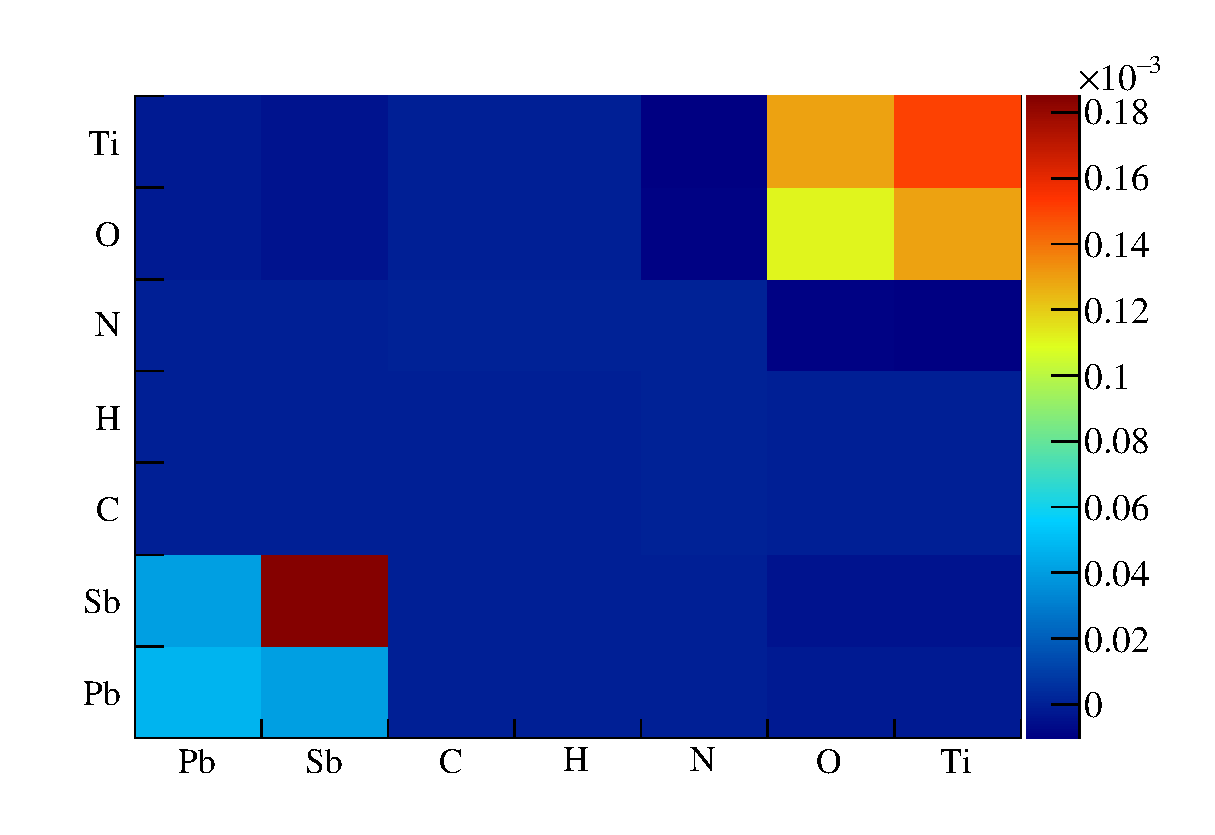
\includegraphics[width=10cm]{images/measurement/systematics/detector/mass/MassCov_DSECal_AllElements.eps}
  \caption{The covariance matrix for the mass of the contributing elements in the DS ECal, with all contributing elements considered.}
  \label{fig:MassCovDSECalAllElements}
\end{figure}
\begin{figure}[b!]
  \centering
  \includegraphics[width=10cm]{images/measurement/systematics/detector/mass/TotalMass_DSECal.eps}
  \caption{The total mass of the DS ECal active volume with (black) and without (blue) nitrogen and hydrogen as contributing elements.  The smooth lines are the Gaussian fits to the distributions.  Using the Gaussian mean and width as the mass central value and uncertainty respectively, the DS ECal active mass with (without) hydrogen and nitrogen is $4060\pm20$~kg ($3960\pm20$~kg).}
  \label{fig:TotalMassDSECal}
\end{figure}
\begin{figure}
\begin{minipage}{.5\linewidth}
  \centering
  \subfloat[Top/bottom ECal.]{\label{fig:MassCovTopBottomECalReducedElements}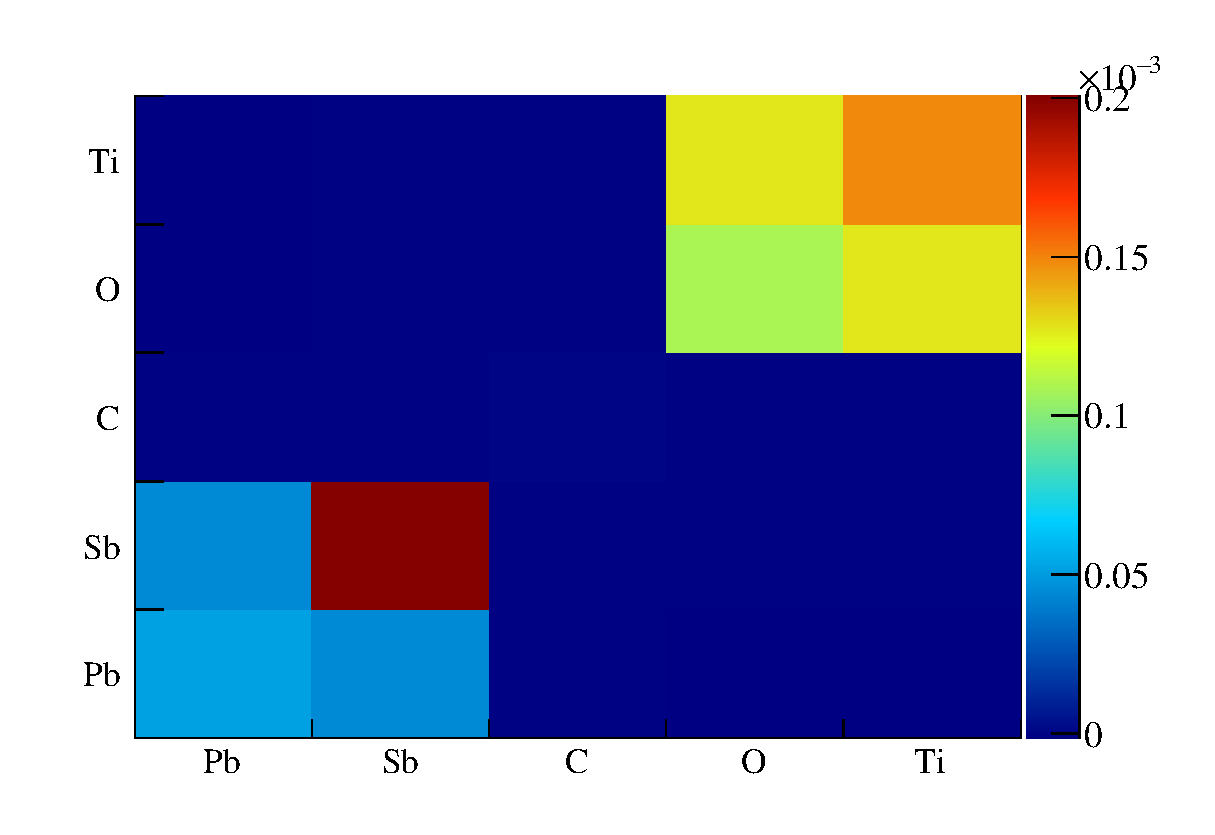
\includegraphics[width=7.5cm]{images/measurement/systematics/detector/mass/MassCov_TopBottomECal_ReducedElements.eps}}
\end{minipage}%
\begin{minipage}{.5\linewidth}
\centering
 \subfloat[Side ECal.]{\label{fig:MassCovSideECalReducedElements}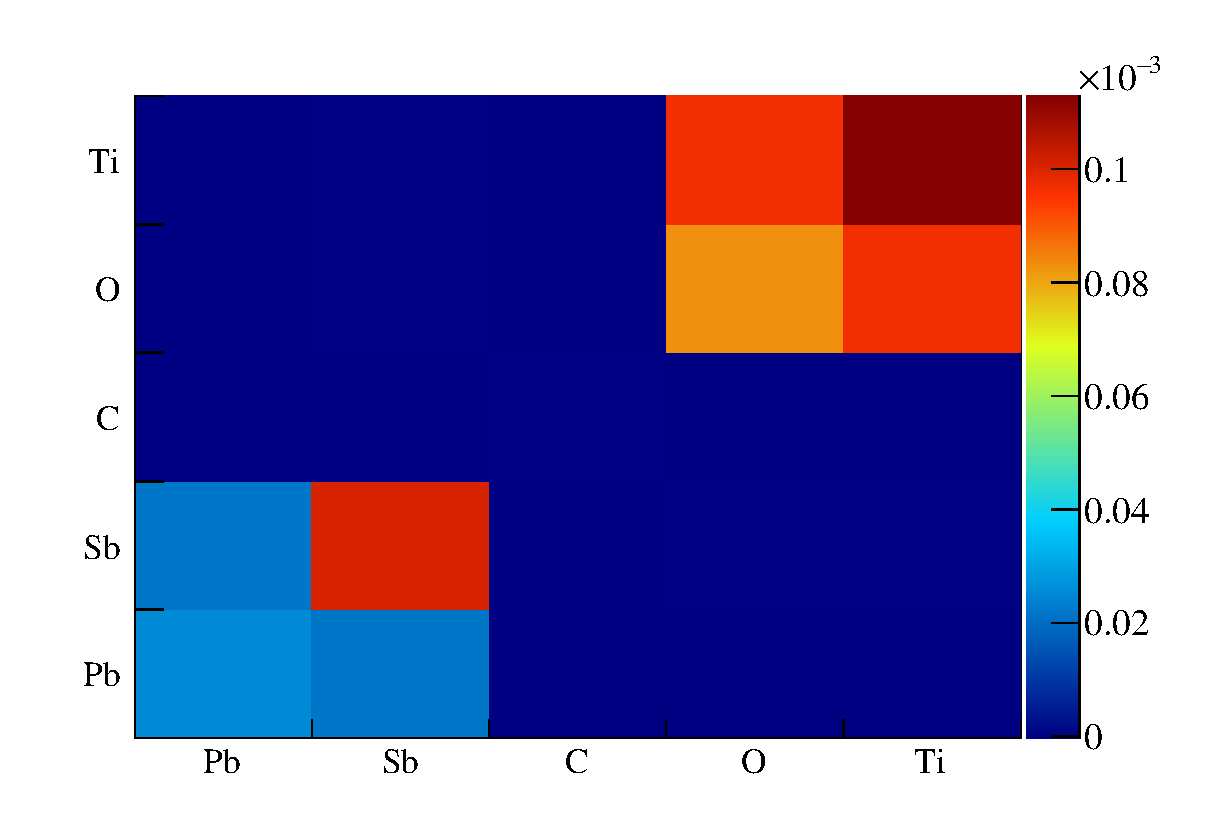
\includegraphics[width=7.5cm]{images/measurement/systematics/detector/mass/MassCov_SideECal_ReducedElements.eps}}

\end{minipage}\par\medskip
\centering
 \subfloat[DS ECal.]{\label{fig:MassCovDSECalReducedElements}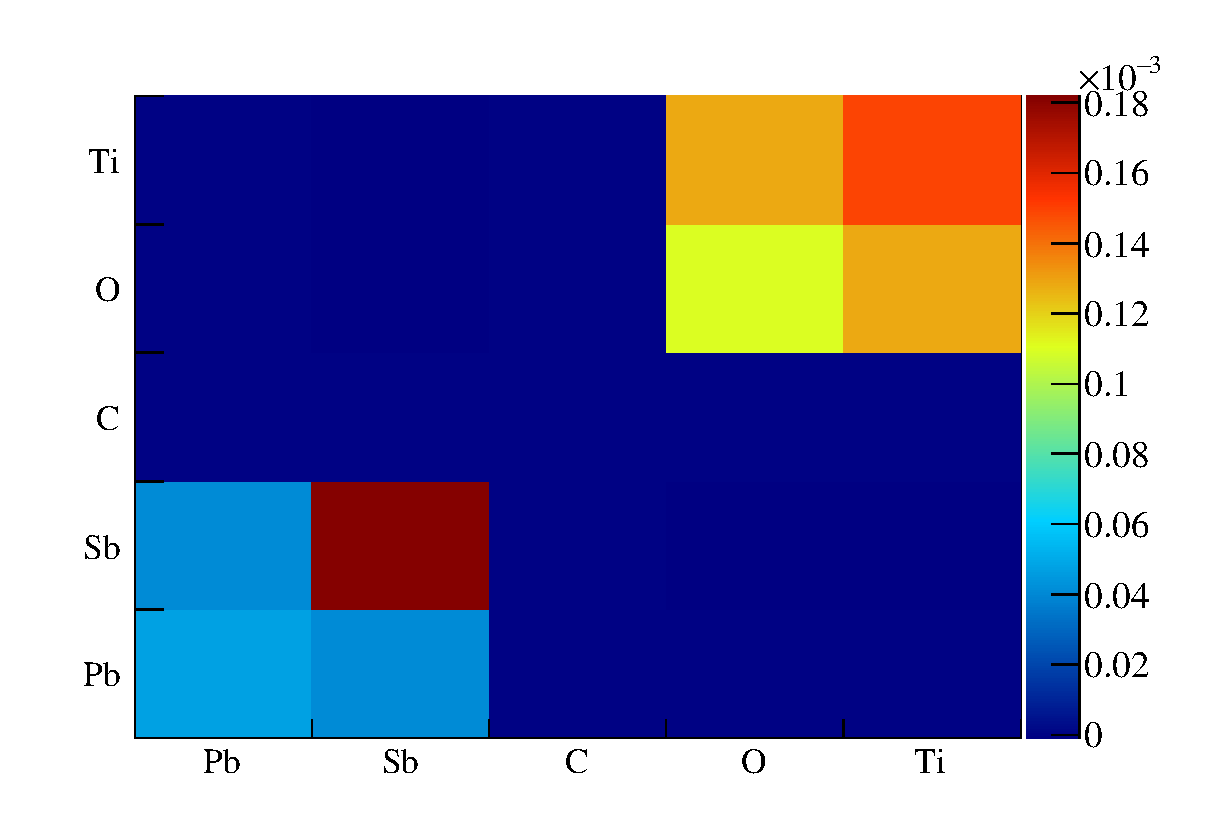
\includegraphics[width=7.5cm]{images/measurement/systematics/detector/mass/MassCov_DSECal_ReducedElements.eps}}

\caption{The fractional covariance matrix for the mass of each contributing element to an ECal module (hydrogen and nitrogen omitted).}
\label{fig:MassCovECalReducedElements}
\end{figure}
\subsubsection{Propagation of the mass systematic uncertainty}
\label{subsubsec:ECalMassSystematicPropagation}
The covariance matrices shown in Fig.~\ref{fig:MassCovECalReducedElements} were then used to generate systematic throws, in the same manner as the flux systematic uncertainty evaluation.  For the input into each systematic throw i.e. one run through of the selected Monte Carlo events, a set of event weights were generated for each of the seven ECal modules using the above mass covariance matrices.  Every neutrino interaction in the ECal active volume was weighted according to its target element.  As with the other systematic uncertainty evaluations, 1,000 systematic throws were generated and the subsequent covariance matrices were constructed which are shown in Fig.~\ref{fig:ECalMassCovarianceMatrices}.  The maximum uncertainty, which was for the DS ECal events, was found to be $0.39\%$. 
\begin{figure}%
  \centering
  \subfloat[Shape+normalisation.]{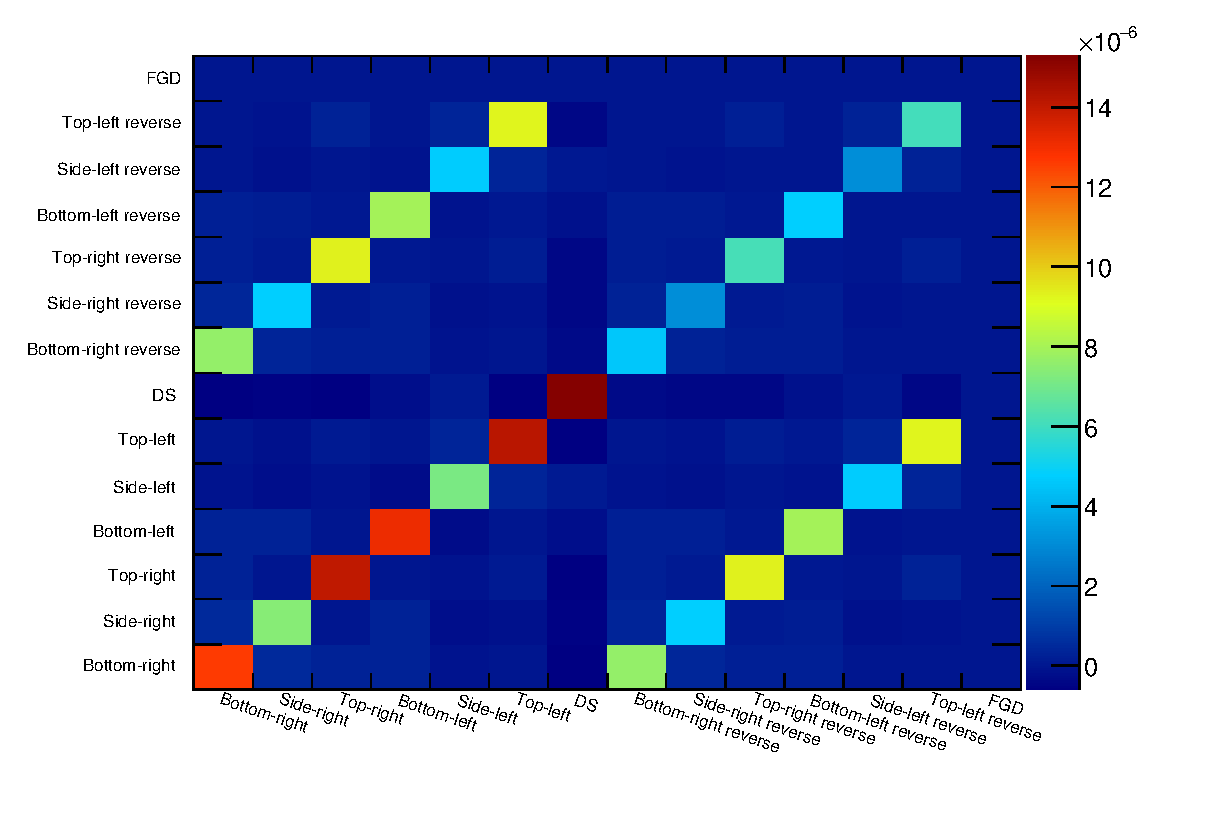
\includegraphics[width=8cm]{images/measurement/systematics/detector/mass/ecal_mass_covariance_matrix.eps} \label{fig:ECalMassShapeNormCovarianceMatrix}}
  \subfloat[Shape-only.]{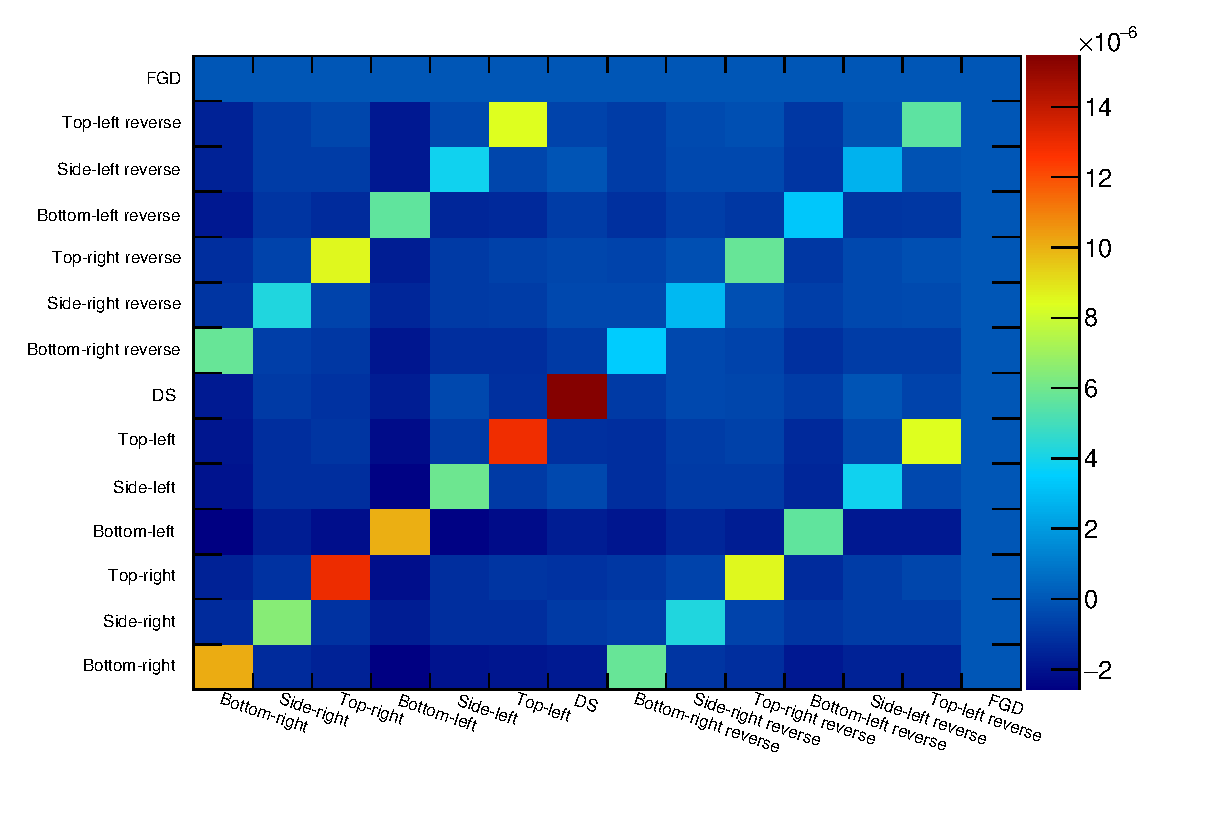
\includegraphics[width=8cm]{images/measurement/systematics/detector/mass/ecal_mass_shape_covariance_matrix.eps} \label{fig:ECalMassShapeOnlyCovarianceMatrix}}
  \caption{The sample covariance induced by the ECal mass uncertainties.}
  \label{fig:ECalMassCovarianceMatrices}
\end{figure}
\newline
\newline
An additional source of systematic uncertainty could come from the ECal's ability to reject OOFV backgrounds. As fig.~\ref{fig:ProngStackSelected} shows, the dominant background selected, particularly for the barrel ECals, is the OOFV background.  If the simulation of the ECal had a different OOFV background rejection capability to that of the actual ECal, the selected event composition between data and MC would differ, resulting in a systematic difference.  The only feasible way to assess this systematic uncertainty is to use control samples.  Unfortunately, only $\mu$ based control samples were available during the analysis.  However, fig,~\ref{fig:ProngStackSelected} shows that the one prong topology, which contains the largest number of selected events, has the biggest OOFV background contamination and as Fig.~\ref{fig:SelOOFVEventSurvivalBarrel} and Fig.~\ref{fig:SelOOFVEventSurvivalDS} show, $\mu$s are the dominant particle species in the surviving OOFV background.  To assess the systematic uncertainty, the $\mu$ based control samples, both data and MC, were passed through the selection and the number of reconstructed events which pass the fiducial volume cut were recorded, $N_{\textrm{CS}}^{\textrm{pass}}$.  The efficiency of the fiducial volume cut was then defined as
\begin{equation}
\epsilon_{\textrm{CS}} = \frac{N_{\textrm{CS}}^{\textrm{pass}}}{N_{\textrm{CS}}},
\label{eqn:OOFVCSEfficiency}
\end{equation}
where $N_{\textrm{CS}}$ is the number of reconstructed control sample events which enter the selection.  It is important to note why $N_{\textrm{CS}}^{\textrm{pass}}$ counts the number of events which pass the fiducial volume cut, rather than as the number of events which pass all of the selection cuts.  The reason for this is the inclusion of the reverse sample (background\Yoshi{-}{ADDRESSED - compound adjective}enriched sample) in the rate fit which includes any event which passes the fiducial volume cut, but fails the most upstream cut.  By calculating $\epsilon_{\textrm{CS}}$ separately for data and MC, the systematic uncertainty can then be defined as
\begin{equation}
\alpha_{\textrm{OOFV}} = \epsilon_{\textrm{CS}}^{\textrm{data}} - \epsilon_{\textrm{CS}}^{\textrm{MC}}.
\label{eqn:OOFVSystematic}
\end{equation}
The FGD cosmic control samples were used for this study, which are events with coincident reconstructed tracks in both FGDs and which occur outside of a beam spill window.  A summary of the information relevant for systematic uncertainty is located in table~\ref{table:OOFVSystematicSummary}.  
\begin{table}
  \begin{tabular}{ c c c c c c }
    ECal module(s) & $N_{\textrm{CS}}$ (MC) & $N_{\textrm{CS}}$ (data) & $\epsilon_{\textrm{CS}}$ (MC) & $\epsilon_{\textrm{CS}}$ (data) & $\alpha_{\textrm{OOFV}}$ \\ \hline \hline
    Barrel & 26560 & 42961 & 2.12$\%$ & 5.92$\%$ & 3.80$\%$ \\
    DS & 6225 & 22555 & 2.27$\%$ & 5.97$\%$ & 3.70$\%$ \\
  \end{tabular}
  \caption{Summary of the ECal OOFV systematic study when using the FGD cosmic control sample.}
  \label{table:OOFVSystematicSummary}
\end{table}
\newline
\newline
To propagate the effect of the systematic uncertainty, a similar approach to the flux systematic uncertainty propagation.  However, as the OOFV systematic uncertainty is a pair of single numbers rather than a covariance matrix, only two event weights (one for the barrel ECal and one for the DS ECal) were generated per systematic throw.  The event weights were used to reweight only the OOFV events in the sample and the subsequent sample covariance matrices were constructed, which are shown in Fig.~\ref{fig:ECalOOFVCovarianceMatrices}.  The largest uncertainty is in the bottom-left reverse sample and is 1.82$\%$.
\begin{figure}[t!]
  \centering
  \subfloat[Shape+normalisation.]{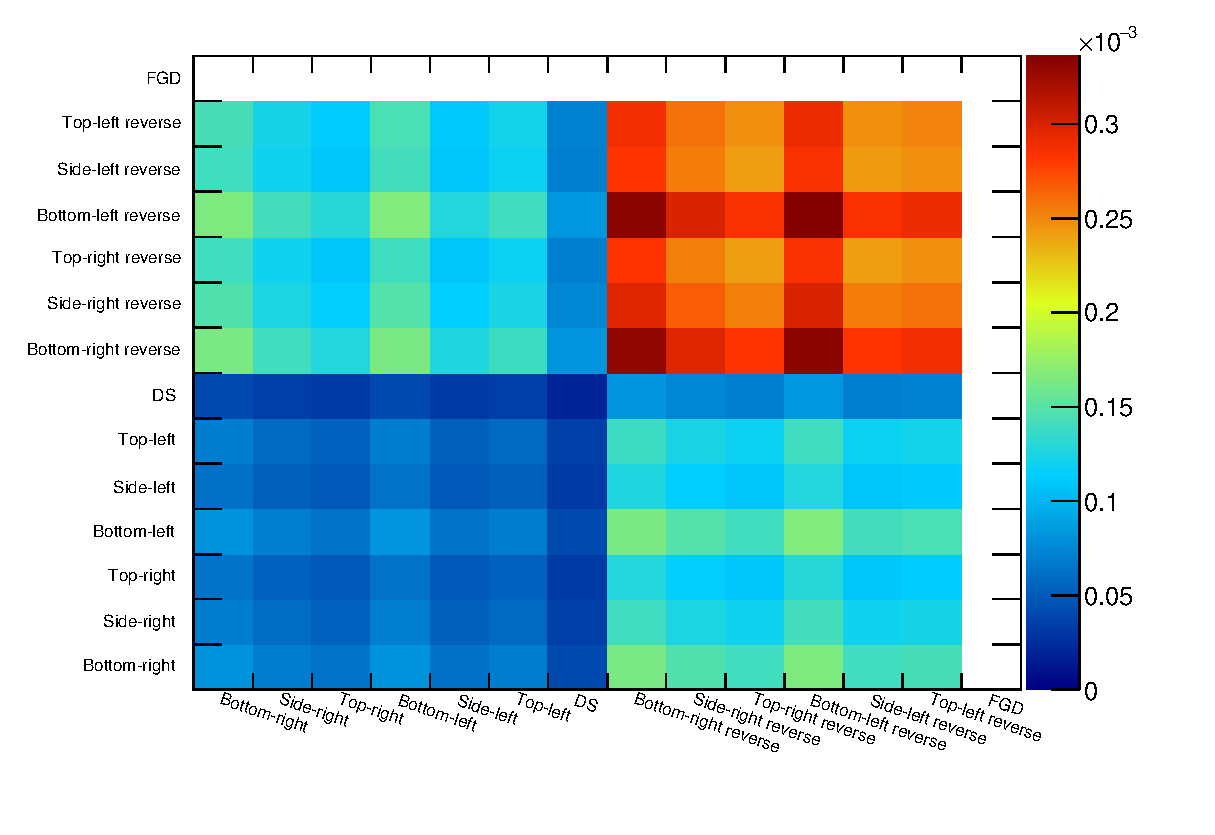
\includegraphics[width=8cm]{images/measurement/systematics/detector/oofv/ecal_oofv_covariance_matrix.eps} \label{fig:ECalOOFVShapeNormCovarianceMatrix}}
  \subfloat[Shape-only.]{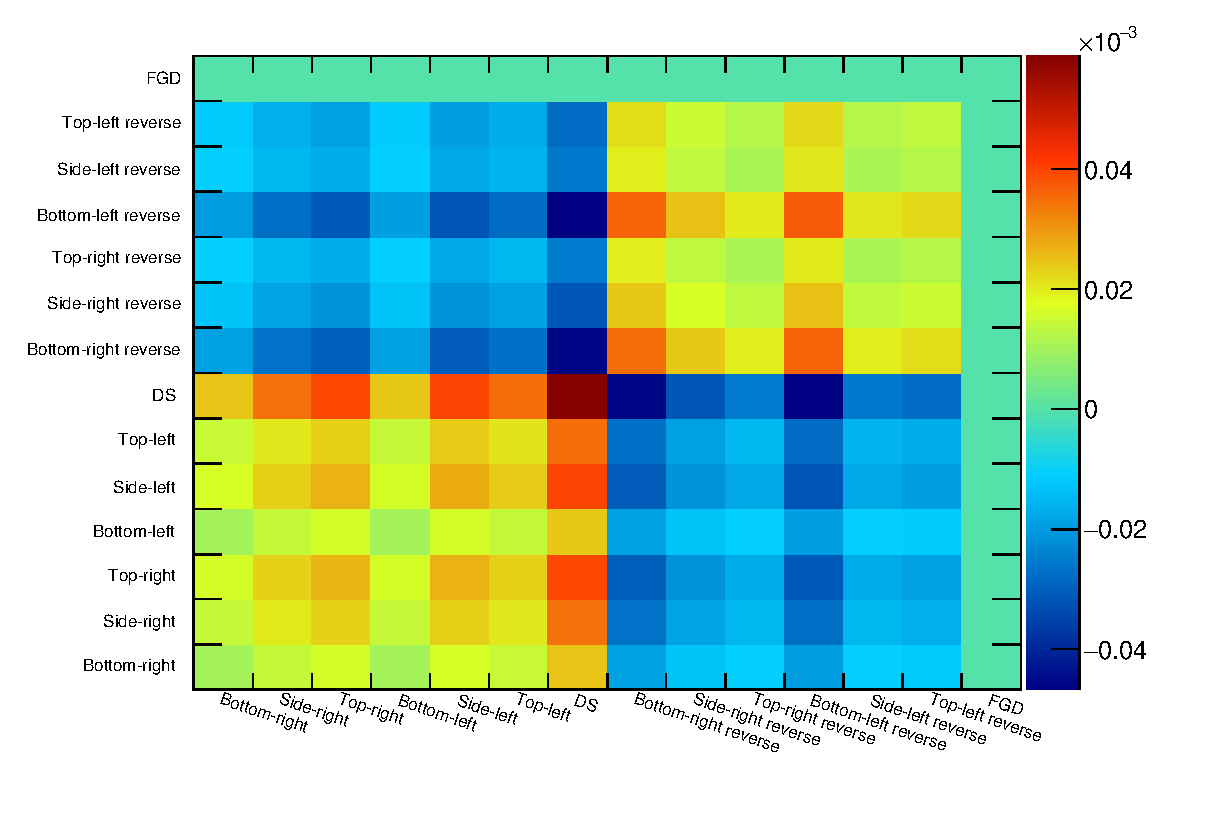
\includegraphics[width=8cm]{images/measurement/systematics/detector/oofv/ecal_oofv_shape_covariance_matrix.eps} \label{fig:ECalOOFVShapeOnlyCovarianceMatrix}}
  \caption{The sample covariance induced by the uncertainty in the ECal OOFV events.}
  \label{fig:ECalOOFVCovarianceMatrices}
\end{figure}
\newline
\newline
As described in section~\ref{sec:ReconstructionValidation}, a significant data/MC difference was found in the DS ECal reconstructed events when looking at the through-going muon control sample.  The 2D reconstructed track quality check required that tracks contained no layer gaps.  There was an unforeseen hit inefficiency in the DS ECal which was not modelled in MC, which would cause tracks to be rejected because of the 2D track quality check (see section~\ref{subsec:DataMotivatedValidation}).  Because this problem was found after significant progress had been made on the MC selection, it was decided that this bug would be treated as a systematic uncertainty in the analysis.  To assess this ad hoc systematic uncertainty, the quality check was relaxed to allow 2D tracks to skip one layer in a given view.  The reconstruction and selection was then applied to the sample and was compared to the nominal sample to construct the covariance matrices, which are shown in Fig.~\ref{fig:ECalHoughBugCovarianceMatrices}.
\begin{figure}[b!]
  \centering
  \subfloat[Shape+normalisation.]{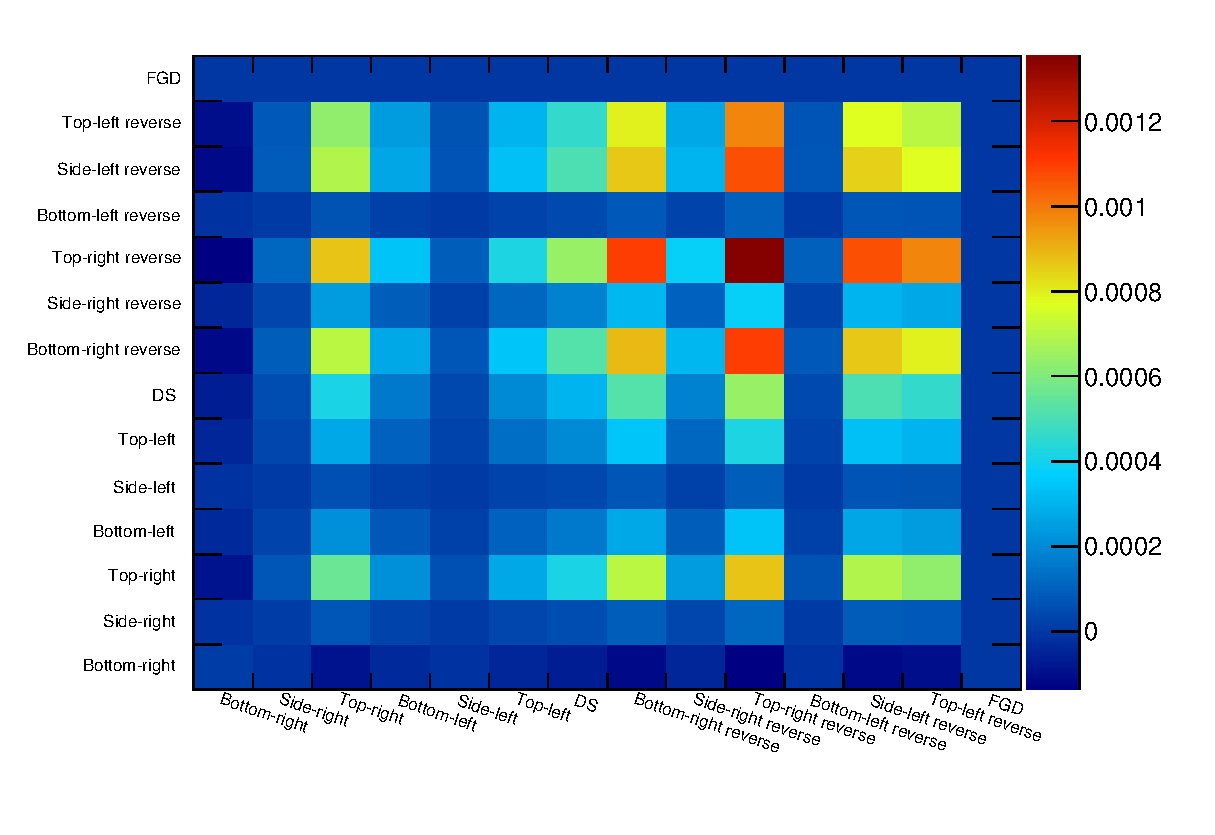
\includegraphics[width=8cm]{images/measurement/systematics/detector/bug/ecal_hough_covariance_matrix.eps} \label{fig:ECalHoughBugShapeNormCovarianceMatrix}}
  \subfloat[Shape-only.]{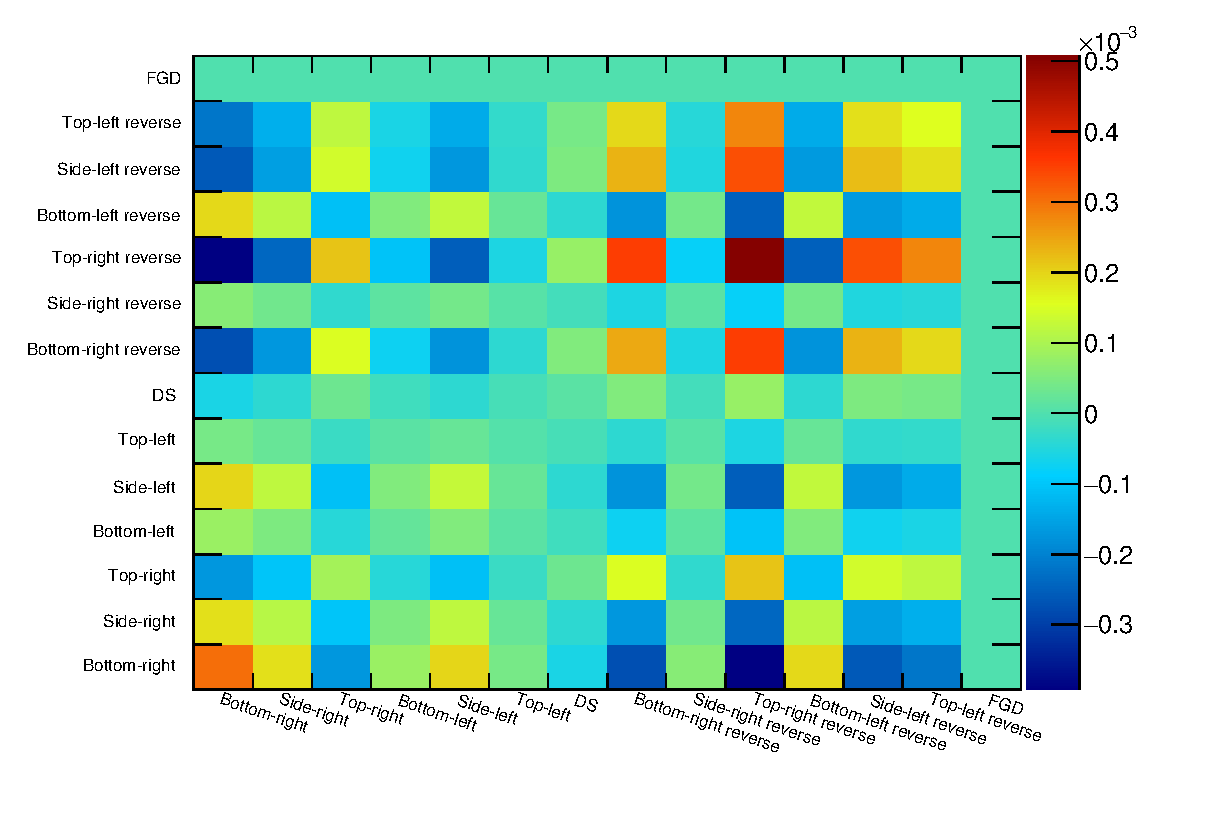
\includegraphics[width=8cm]{images/measurement/systematics/detector/bug/ecal_hough_shape_covariance_matrix.eps} \label{fig:ECalHoughBugShapeOnlyCovarianceMatrix}}
  \caption{The sample covariance induced by the bug fix to the reconstruction.}
  \label{fig:ECalHoughBugCovarianceMatrices}
\end{figure}
\subsection{FGD detector uncertainty evaluation}
\label{subsec:FGDDetectorSystematics}
The systematic uncertainties associated with the FGD are described extensively in~\cite{CCIncSelFGDTN}.  In recent times, there has been a significant push to develop a framework in which to analyse and propagate systematic uncertainties associated with ND280 analyses, which is called the PSYCHE framework.  Even though outer detector analyses have not been incorporated into PSYCHE, this is not true for Tracker analyses and so PSYCHE could be partly utilised in this analysis.  The design of PSYCHE allows the user to enable/disable relevant systematic uncertainties and then simultaneously propagate them through an analysis.  PSYCHE was set up to apply the FGD detector systematics and produce 1000 throws, in which every systematic uncertainty was simultaneously applied.  The output, in the form of a distribution of a varied number of selected CC events in the FGD, was then used to define the systematic uncertainty.  This distribution is shown in Fig.~\ref{fig:FGDSystematicsNEvents}.  The Gaussian fit to the thrown number of events implies that the number of FGD events is $(1.069\pm0.022)\times10^5$ events i.e. a $2.01\%$ uncertainty.  However, the number of nominal selected events is $1.054\times10^5$ and so the shift in the number of events suggests an additional $1.41\%$ error.  Combining these in quadrature, the FGD detector systematic uncertainty was found to be $2.51\%$.  This error purely relates to the number of CC events in the FGD and so does not correlate with any of the events in the ECal.
\begin{figure}
  \centering
  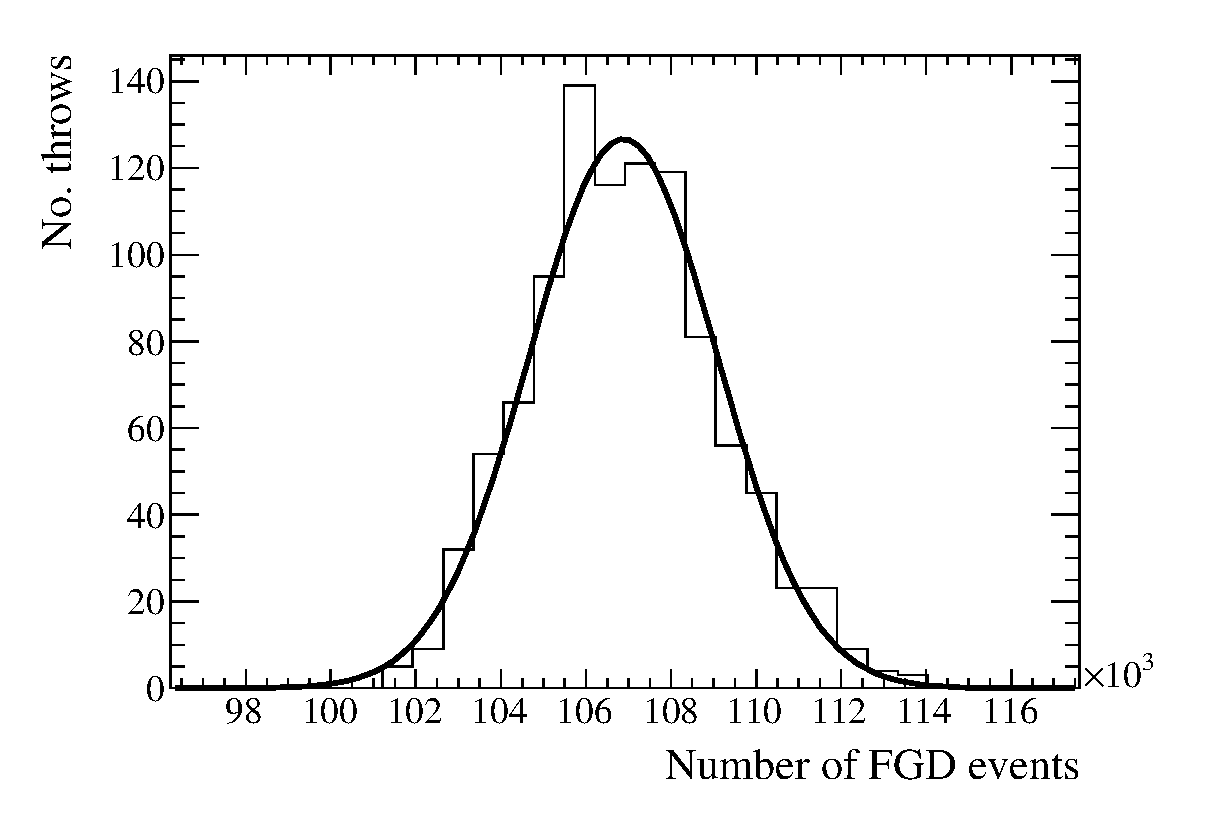
\includegraphics[width=10cm]{images/measurement/systematics/detector/fgd/fgd_systematics_nevents.eps}
  \caption{The number of selected FGD events for each systematic throw using PSYCHE.  The smooth line is a Gaussian fit to the number of events.}
  \label{fig:FGDSystematicsNEvents}
\end{figure}
\newline
\newline
The total detector covariance matrices are shown in Fig.~\ref{fig:DetectorCovarianceMatrices}.  These matrices were found by summing all of the detector related covariance matrices.  The exception to this is the FGD detector uncertainty in which the single variance was added to the FGD on-diagonal bin.  The largest uncertainty was found to be $5.04\%$.
\begin{figure}%
  \centering
  \subfloat[Shape+normalisation.]{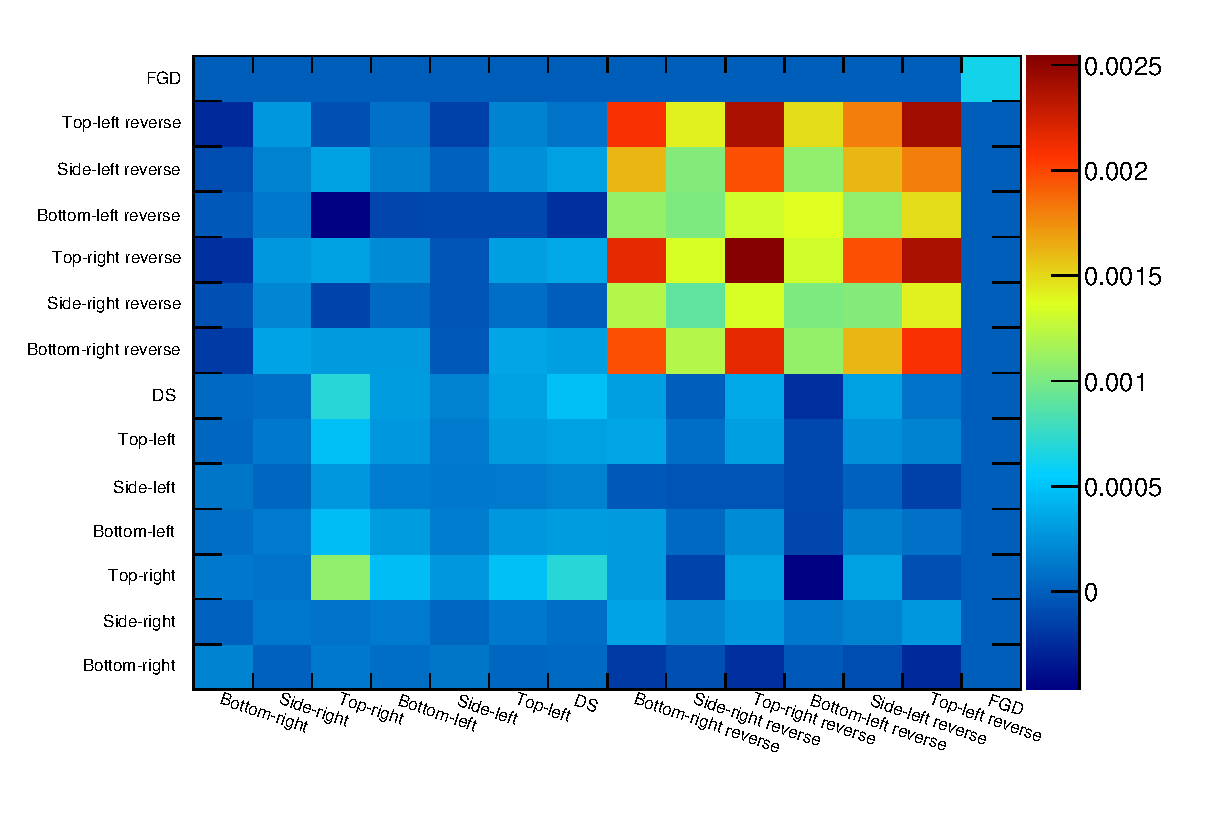
\includegraphics[width=8cm]{images/measurement/systematics/detector/total/detector_covariance_matrix.eps} \label{fig:DetectorCovarianceMatrix}}
  \subfloat[Shape-only.]{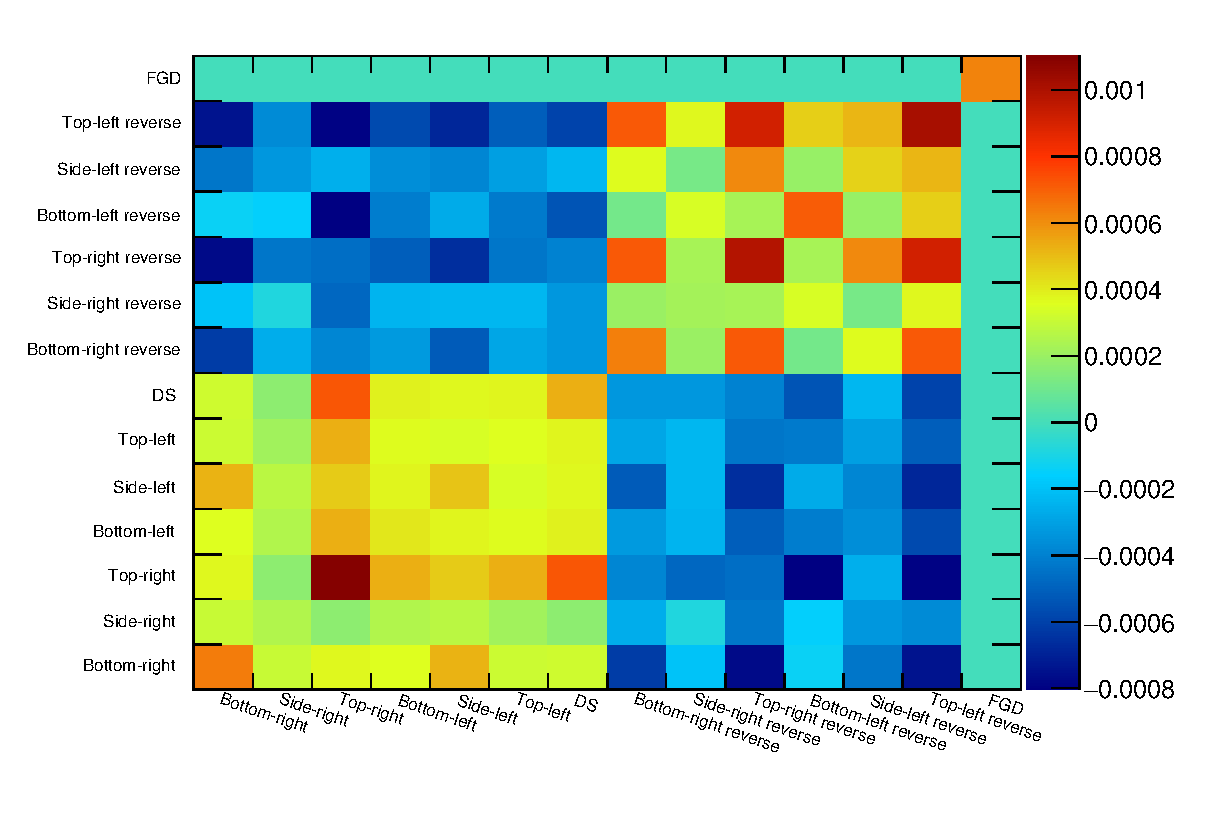
\includegraphics[width=8cm]{images/measurement/systematics/detector/total/detector_shape_covariance_matrix.eps} \label{fig:DetectorShapeCovarianceMatrix}}
  \caption{The sample covariance induced by all of the detector related uncertainties.}
  \label{fig:DetectorCovarianceMatrices}
\end{figure}
The total covariance matrices, combining all of the covariance matrices discussed above, are shown in Fig.~\ref{fig:TotalCovarianceMatrices}.  The largest uncertainty is $13.8\%$.
\begin{figure}%
  \centering
  \subfloat[Shape+normalisation.]{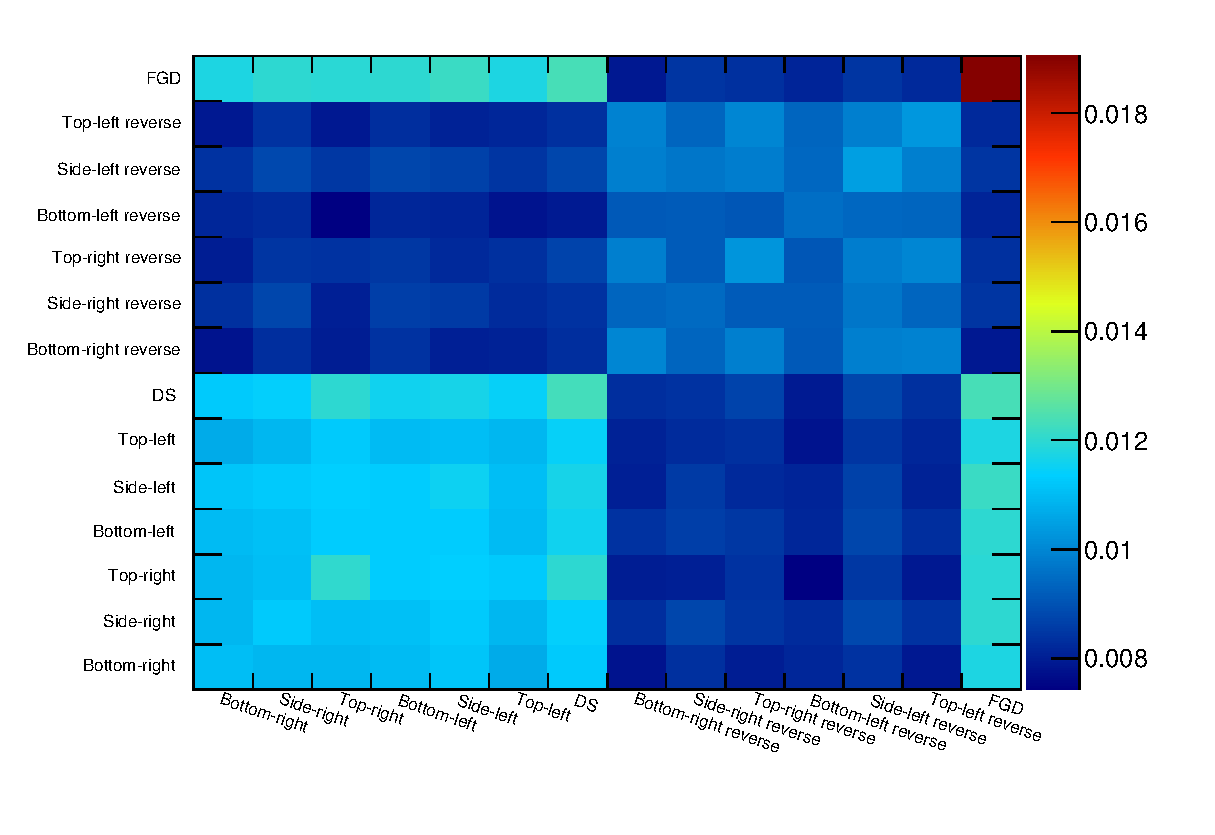
\includegraphics[width=8cm]{images/measurement/systematics/total/total_covariance_matrix.eps} \label{fig:TotalCovarianceMatrix}}
  \subfloat[Shape-only.]{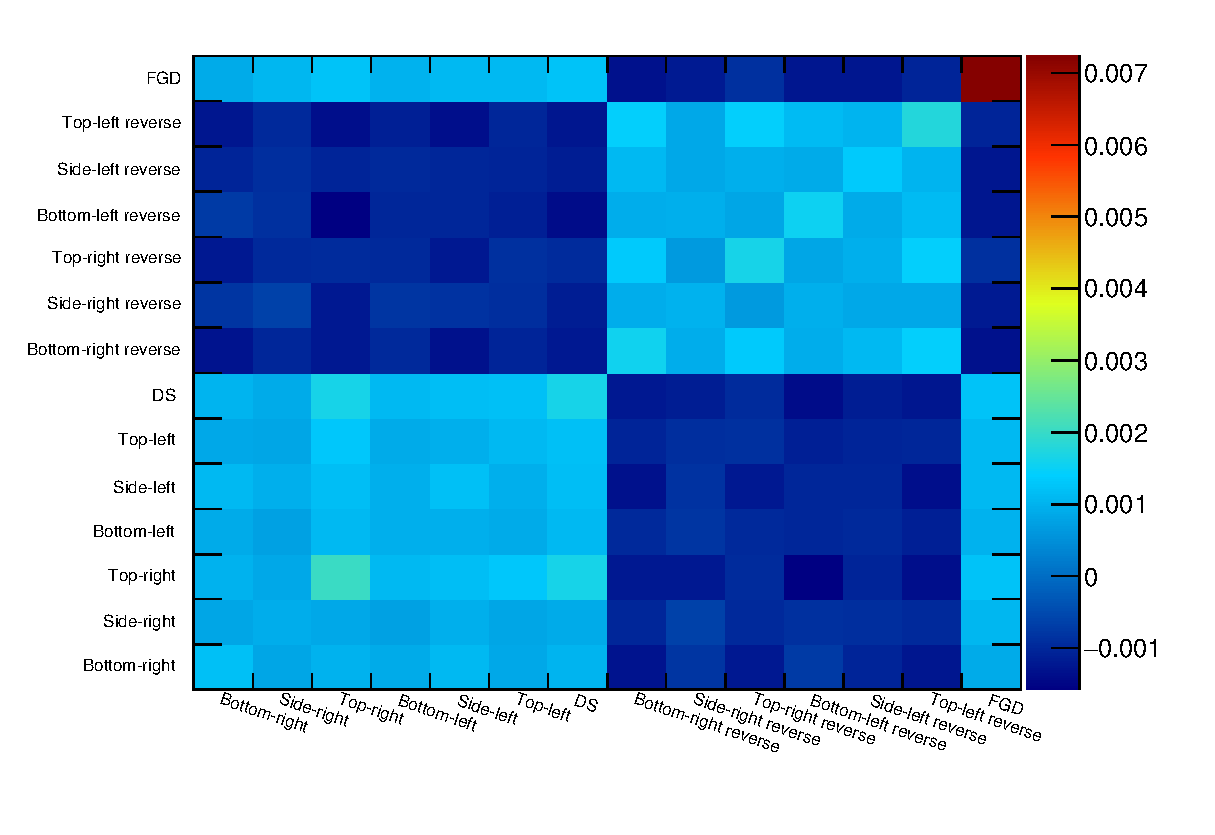
\includegraphics[width=8cm]{images/measurement/systematics/total/total_shape_covariance_matrix.eps} \label{fig:TotalShapeCovarianceMatrix}}
  \caption{The sample covariance induced by all of the systematic uncertainties.}
  \label{fig:TotalCovarianceMatrices}
\end{figure}
\newline
\newline
The selection presented in chapter~\ref{chap:NeutrinoInteractionSelection} heavily used Monte Carlo simulation of neutrino interactions to estimate the efficiency of the selection.  At the core of the simulation, NEUT was used to initially generate the simulated neutrino interactions.  Ideally, the selection efficiency should be a property of the selection itself.  However, because of the use of a neutrino generator in the simulation, it is possible that the selection could contain an element of generator dependency.  It is non-trivial to use a data control sample to assess a systematic uncertainty on the selection efficiency.  In fact, the only feasible way to address this analysis issue would be to use multiple neutrino generators as inputs to the same ND280 simulation and compare the differences.  Unfortunately, a large set of generators were not available for use in the time frame of the analysis.  In ND280 software productions, a large amount of neutrino events based on the GENIE neutrino generator~\cite{Andreopoulos201087} are produced, separately to the NEUT events.  So $2.5\times 10^{19}$~POT worth of GENIE events were passed through the ND280 software chain (including the enhanced reconstruction) and the selection presented in chapter~\ref{chap:NeutrinoInteractionSelection}.  No GENIE-based sand MC has ever been produced in ND280 software productions.  However, as this check only concerns changes to the selection efficiency, an absence of sand MC should not be a problem.  
\newline
\newline
The selected events distributions, separated into the prong topologies, are shown in Fig.~\ref{fig:ProngStackSelectedGENIE}.  The selection efficiencies for each prong topology are shown in Fig.~\ref{table:SelEfficiencyGENIE}.  As described in section~\ref{subsec:SelectionPerformance}, the selection efficiencies do not include neutrino events which were not reconstructed.  So, the topology combined efficiencies which do include said events are shown in table~\ref{table:FinalEffGENIE}.
\begin{figure}
  \centering
  \subfloat[Barrel ECals.]{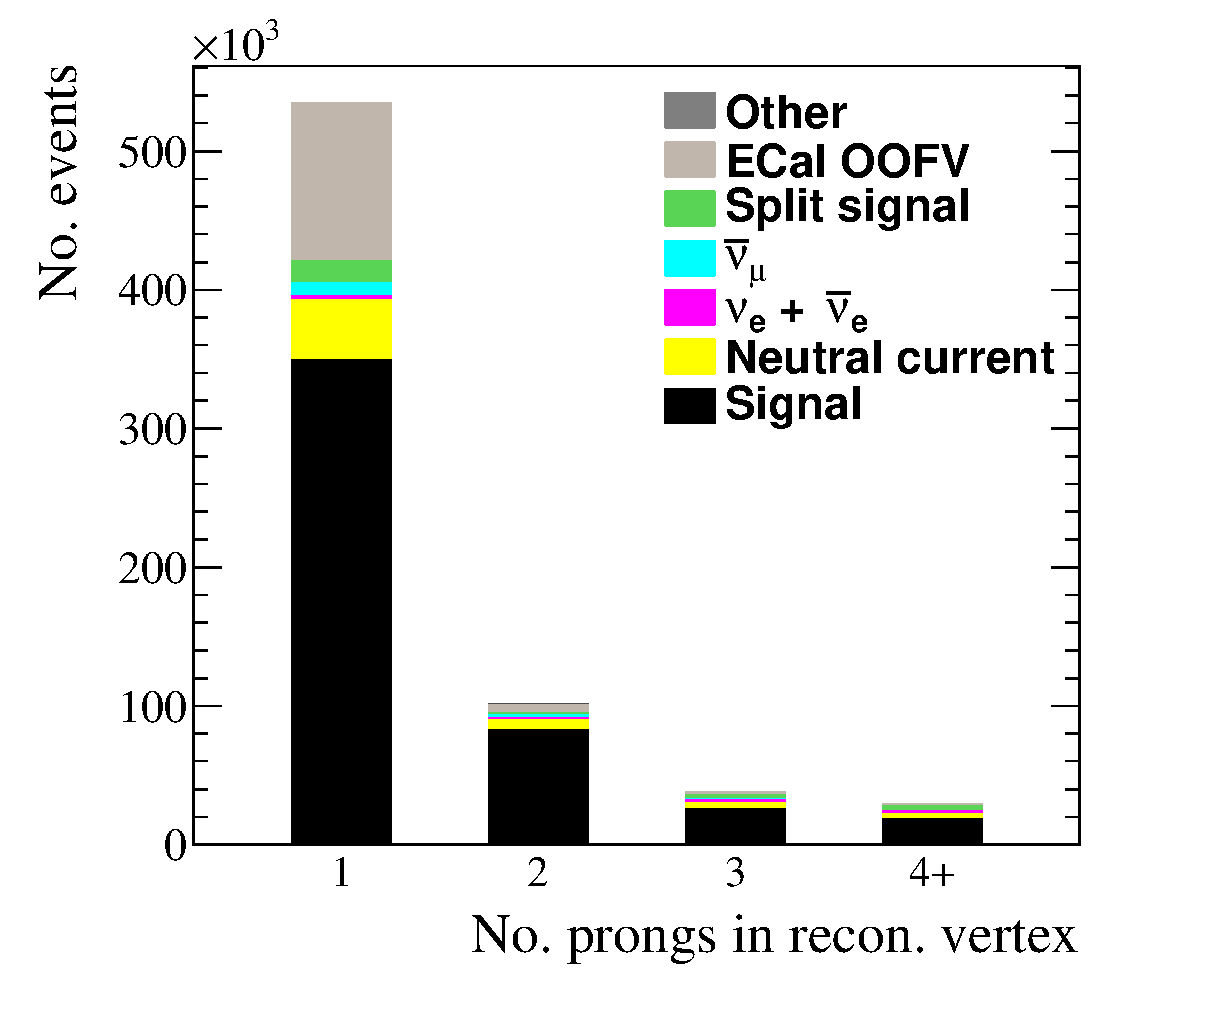
\includegraphics[width=9cm]{images/measurement/systematics/genie/ProngStack_Barrel_Selected_GENIE.eps} \label{fig:ProngStackBarrelSelectedGENIE}}
  \subfloat[DS ECal.]{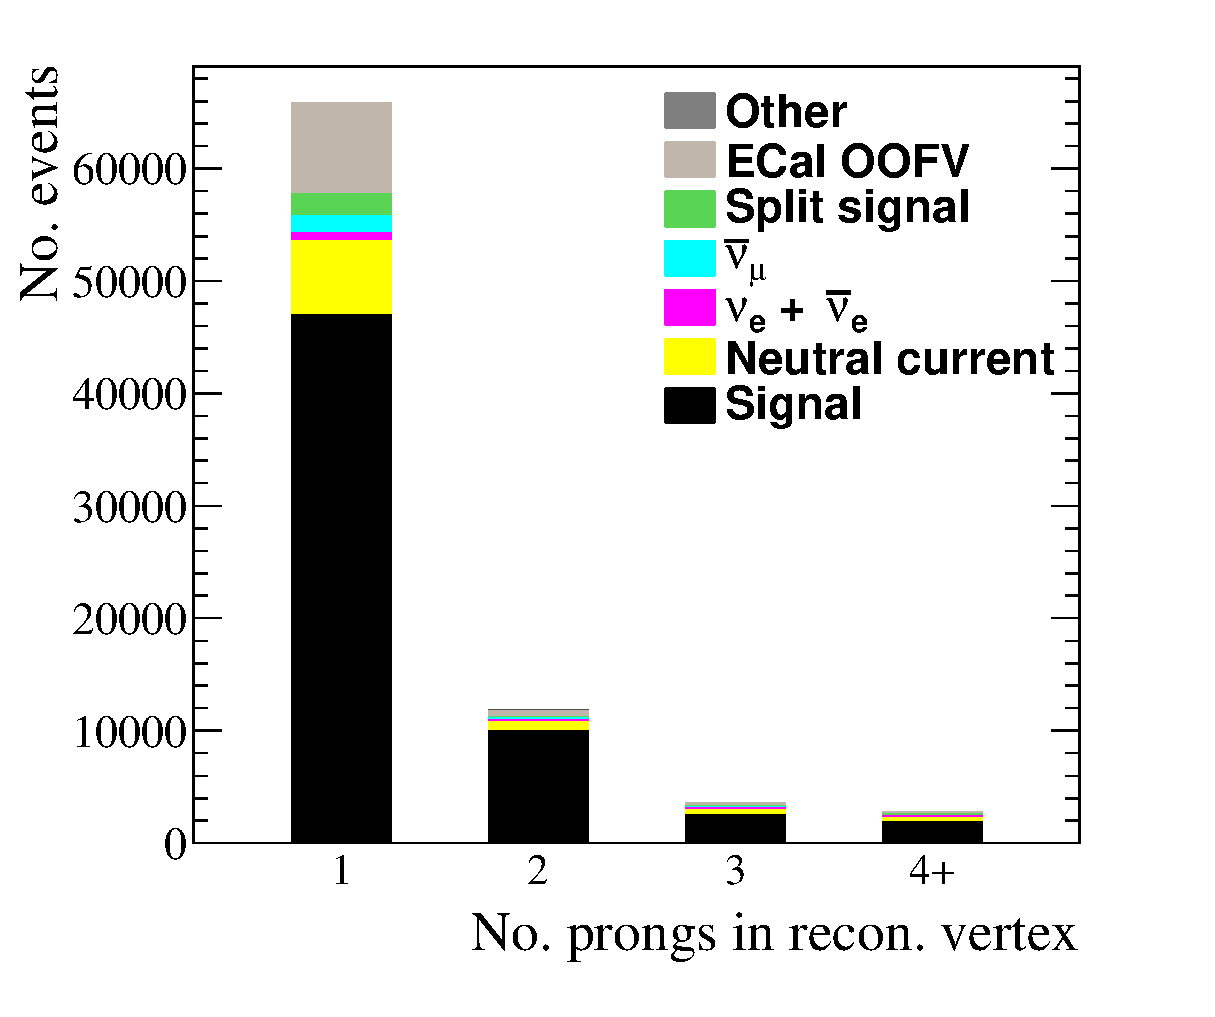
\includegraphics[width=9cm]{images/measurement/systematics/genie/ProngStack_DS_Selected_GENIE.eps} \label{fig:ProngStackDSSelectedGENIE}}
  \caption{The number of selected events in the GENIE-based Monte Carlo sample, separated out into the prong topologies.  Each event is categorised by the associated truth information from the simulation.}
  \label{fig:ProngStackSelectedGENIE}
\end{figure}
\begin{table}
  \begin{tabular}{ c c c c c }
    ECal & 1 prong topology & 2 prong topology & 3 prong topology & 4+ prong topology \\
    module & efficiency ($\%$)& efficiency ($\%$)& efficiency ($\%$)& efficiency ($\%$) \\ \hline \hline
    Barrel & 46.3 & 54.2 & 66.0 & 65.4 \\
    DS & 55.9 & 58.3 & 59.5 & 59.9\\
  \end{tabular}
  \caption{The selection efficiencies from the GENIE-based Monte Carlo sample for each prong topology and ECal module.}
  \label{table:SelEfficiencyGENIE}
\end{table}
\begin{table}
  \begin{tabular}{ c c }
    ECal module & Efficiency ($\%$) \\ \hline \hline
    Barrel & 40.7 \\
    DS & 49.9  \\
  \end{tabular}
  \caption{The topology combined efficiency for the GENIE-based Monte Carlo sample.  The efficiency values include simulated events which were not reconstructed.}
  \label{table:FinalEffGENIE}
\end{table}
\newline
\newline
Overall, there are differences in the selection efficiencies between NEUT and GENIE, particularly for the DS ECal.  However, when combining the topologies and including the events below reconstruction threshold, the efficiency differences are somewhat minor.  As described at the start of this chapter, the DS ECal will form the primary target and so it is the DS ECal efficiency which is the most important.  The DS ECal efficiency uncertainty is simply defined as the difference between the NEUT and GENIE efficiencies, which is $53.0\% - 49.9\% = 3.1\%$.  This error as a fraction of the nominal uncertainty is $5.85\%$.
\subsection{The measured cross-section uncertainty}
Using all of the information described in chapter~\ref{chap:NeutrinoInteractionSelection} and chapter~\ref{chap:CrossSectionMeasurement}, the $\nu_\mu$ CC-inclusive cross-section on lead will be calculated as
\begin{equation}
\label{eq:CrossSection}
\sigma^{\textrm{CC}}_{\textrm{Pb}} = \frac{R_{\textrm{Pb}}N^{\textrm{MC}}_{\textrm{Pb}}\eta_{\textrm{Pb}}}{T_{\textrm{Pb}}\Phi^{\textrm{MC}}\epsilon_{\textrm{Pb}}},
\end{equation}
where $R_{\textrm{Pb}}$ is the Pb normalisation returned from the rate fit, $N^{\textrm{MC}}_{\textrm{Pb}}$ is the number of selected events in the DS ECal, $T_{\textrm{Pb}}$ is the number of Pb nuclei present in the DS ECal, $\Phi^{\textrm{MC}}$ is the total flux used to create the MC and $\eta_{\textrm{Pb}}$ and $\epsilon_{\textrm{Pb}}$ are the purity and efficiency of the DS ECal selection.  The shape covariance matrix (shown in Fig.~\ref{fig:TotalShapeCovarianceMatrix}) will be used as an input to the fit.  This covariance matrix includes uncertainties on the flux and (partly) on the number of Pb nuclei.  Therefore, the error on $R_{\textrm{Pb}}$ will provide the error from the shape systematic uncertainties which means it is only necessary to include a couple of extra uncertainties on the actual measurement of the cross-section.  It is necessary to include the normalisation uncertainty on the number of selected DS ECal events.  This value, taken from Fig.~\ref{fig:TotalCovarianceMatrix} is $11.1\%$.  The error on the efficiency, as discussed above, is $5.85\%$. Despite having investigated systematic differences in the ECal mass, the simulation does not include antimony in the absorber sheets.  The absorber sheets are quoted as having a $0.2\%$ uncertainty on the antimony doping~\cite{1748-0221-8-10-P10019} which also needs to be included in the final uncertainty.  Combining all of this information, the final uncertainty on the measured cross-section will be
\begin{equation}
\label{eq:CrossSectionUncertainty}
\sigma_{\sigma^{\textrm{CC}}_{\textrm{Pb}}} = \sigma_{R_{\textrm{Pb}}} \pm 12.5\%,
\end{equation}
where $\sigma_{R_{\textrm{Pb}}}$ is the error on $R_{\textrm{Pb}}$ returned from the rate fit.

\section{Validation of method}
\label{sec:MethodValidation}
The ECal rate fit described in section~\ref{sec:ECalRateFit} requires validation to ensure that not only the machinery works as intended, but also to check that the fit is suitable for such an analysis.  The first set of validation checks performed deals with the former case.

\subsection{Validation of the fit machinery}
\label{subsec:FitMachineryValidation}
The initial validation method used the same Monte Carlo described in section~\ref{sec:InputSamples} to create toy datasets which were passed through the fitter.  To create said datasets, new normalisation parameters, $R^{\textrm{Val}}$, were defined which are shown in table~\ref{table:ValidationNormalizationSets}.  These new normalisation parameters scale the relevant Monte Carlo templates.  
\begin{table}
  \begin{tabular}{c | c c c }
    Normalisation set & $R^{\textrm{Pb}}$ & $R^{\textrm{C}}$ & $R^{\textrm{Other}}$\\ \hline \hline
    1 & 1.0 & 1.0 & 1.0 \\
    2 & 3.0 & 1.0 & 1.0 \\
    3 & 0.7 & 1.5 & 0.8 \\
    4 & 1.0 & 0 & 1.0 \\
    5 & -0.3 & 1.0 & 1.0 \\
  \end{tabular}
  \caption{The normalisation sets used in the machinery validation of the ECal rate fit.}
  \label{table:ValidationNormalizationSets}
\end{table}
\newline
\newline
For the MC population $\textrm{X}$ in each sub-detector sample $\imath$, the normalisation parameter is applied to create the new population as
\begin{equation}
n^{\textrm{X Val}}_{\imath} = R^{\textrm{X Val}}_{\imath} n^{\textrm{X Nom}}_{\imath},
\label{eq:ValidationScaledPopulation}
\end{equation}
where $n^{\textrm{X Nom}}_{\imath}$ is the number of events in population $\textrm{X}$ of sub-detector sample $\imath$ for the nominal MC.  The total number of events in each sub-detector sample is then constructed as 
\begin{equation}
N^{\textrm{Val}}_{\imath} = \sum^{\textrm{X}} n^{\textrm{X Val}}_{\imath}.
\label{eq:ValidationNEventsDetector}
\end{equation}
The final step in creation of the toy datasets was to vary the total number of events in the sub-detector samples.  The method chosen was the same as that used to generate event weights for the systematic uncertainty studies described in section~\ref{sec:SystematicUncertainties}.  The covariance matrix shown in Fig.~\ref{fig:TotalShapeCovarianceMatrix} was Cholesky decomposed and multiplied by a vector of random numbers, all drawn from a Gaussian of mean 0 and width 1.  The sub-detector sample weights were then created by adding 1 to each element of the multiplied vector.  Each scaled sub-detector sample, $N^{\textrm{Val}}_{\imath}$, was then reweighted by the relevant sample weight.  This toy dataset was then passed to the fitter and its output recorded.  The steps outlined above describe one pass of the fitter.  This process was repeated 10,000 times for each validation normalisation set.
\newline
\newline
The value of $R^{\textrm{Pb}}$ returned for each throw in parameter set 1 is shown in Fig.~\ref{fig:RateFitValParamSet1RPbFit}.  The Gaussian fit quantifies the performance of the fit: the mean specifies the final value and the width specifies a pseudo-error.  To further quantify how well the machinery works, the parameter pull, $P^{\textrm{X}}_{\imath}$, is defined as  
\begin{equation}
P^{\textrm{X}}_{\imath} = \frac{R^{\textrm{X Fit}}_{\imath} - R^{\textrm{X Val}}_{\imath}}{\sigma^{\textrm{X Fit}}_{\imath}},
\label{eq:FitParameterPull}
\end{equation}
where $R^{\textrm{X Fit}}_{\imath}$ and $\sigma^{\textrm{X Fit}}_{\imath}$ are the value and error of parameter $\textrm{X}$ returned from the fit for throw $\imath$ respectively.  The MINOS routine used in the fitter returns asymmetric errors and so care must be taken when deciding which error to use in equation~\ref{eq:FitParameterPull}.  It was decided that the positive error would be used when the fitter returned a value higher than the input.  $P^{\textrm{Pb}}$ for parameter set 1 is shown in Fig.~\ref{fig:RateFitValParamSet1RPbPull}.  The Gaussian fit to this distribution has a width close to, but slightly below, 1.  This suggests that the errors returned by the MINOS routine very slightly overestimate the error, but are still a very good representation of the uncertainty.
\begin{figure}%
  \centering
  \subfloat[The returned parameter for each throw.  The fitted Gaussian has a mean of 1.00 and a width of 0.04.]{\includegraphics[width=8cm]{images/measurement/validation/machinery/rateFitVal_RPbFit_ParamSet1.eps} \label{fig:RateFitValParamSet1RPbFit}}
  \subfloat[The parameter pull for each throw.  The fitted Gaussian has a mean of 0.01 and a width of 0.96.]{\includegraphics[width=8cm]{images/measurement/validation/machinery/rateFitVal_RPbPull_ParamSet1.eps} \label{fig:RateFitValParamSet1RPbPull}}
  \caption{Distributions of $R^{\textrm{Pb}}$ related information returned from the fitter for the 10,000 fake data throws.  The red dashed lines are Gaussian fits to the distributions.}
  \label{fig:RateFitValParamSet1RPb}
\end{figure}
\begin{figure}%
  \centering
  \subfloat[The mean fitted values for each normalisation parameter (black) compared with the input normalisation values (red).]{\includegraphics[width=8cm]{images/measurement/validation/machinery/rateFitVal_FitVals_ParamSet1.eps} \label{fig:RateFitValsParamSet1}}
  \subfloat[The means (black) and widths (blue) of the pull distributions after fitting with a Gaussian.]{\includegraphics[width=8cm]{images/measurement/validation/machinery/rateFitVal_FitPulls_ParamSet1.eps} \label{fig:RateFitPullsParamSet1}}
  \caption{Performance of the fit for the 10,000 fake data sets when using normalisation set 1.}
  \label{fig:RateFitValParamSet1}
\end{figure}
The performance of the fit for all of the normalisations in normalisation set 1 are shown in Fig.~\ref{fig:RateFitValParamSet1}.  In each case, the fitter returns the correct normalisation and the pull characteristics suggest the fit returns the correct error and is unbiased.  The performance of the fit for normalisation sets 2, 3, 4 and 5 are shown in Fig.~\ref{fig:RateFitValParamSet2}, Fig.~\ref{fig:RateFitValParamSet3}, Fig.~\ref{fig:RateFitValParamSet4} and Fig.~\ref{fig:RateFitValParamSet5} respectively.  Generally speaking, the fitter performs well for all of the situations.  It is clear that the output is sensible even when extreme situations are presented (normalisation set 2) as well as when minor shifts are applied to all three parameters (normalisation set 3).  Even in un-physical situations the fitter returns the input correctly (normalisation set 5).  It is only when a template is removed (normalisation set 4) that the fitter becomes biased.  However, as Fig.~\ref{fig:RateFitPullsParamSet4} shows, the bias is minor.
\begin{figure}%
  \centering
  \subfloat[The mean fitted values for each normalisation parameter (black) compared with the input normalisation values (red).]{\includegraphics[width=8cm]{images/measurement/validation/machinery/rateFitVal_FitVals_ParamSet2.eps} \label{fig:RateFitValsParamSet2}}
  \subfloat[The means (black) and widths (blue) of the pull distributions after fitting with a Gaussian.]{\includegraphics[width=8cm]{images/measurement/validation/machinery/rateFitVal_FitPulls_ParamSet2.eps} \label{fig:RateFitPullsParamSet2}}
  \caption{Performance of the fit for the 10,000 fake data sets when using normalisation set 2.}
  \label{fig:RateFitValParamSet2}
\end{figure}
\begin{figure}%
  \centering
  \subfloat[The mean fitted values for each normalisation parameter (black) compared with the input normalisation values (red).]{\includegraphics[width=8cm]{images/measurement/validation/machinery/rateFitVal_FitVals_ParamSet3.eps} \label{fig:RateFitValsParamSet3}}
  \subfloat[The means (black) and widths (blue) of the pull distributions after fitting with a Gaussian.]{\includegraphics[width=8cm]{images/measurement/validation/machinery/rateFitVal_FitPulls_ParamSet3.eps} \label{fig:RateFitPullsParamSet3}}
  \caption{Performance of the fit for the 10,000 fake data sets when using normalisation set 3.}
  \label{fig:RateFitValParamSet3}
\end{figure}
\begin{figure}%
  \centering
  \subfloat[The mean fitted values for each normalisation parameter (black) compared with the input normalisation values (red).]{\includegraphics[width=8cm]{images/measurement/validation/machinery/rateFitVal_FitVals_ParamSet4.eps} \label{fig:RateFitValsParamSet4}}
  \subfloat[The means (black) and widths (blue) of the pull distributions after fitting with a Gaussian.]{\includegraphics[width=8cm]{images/measurement/validation/machinery/rateFitVal_FitPulls_ParamSet4.eps} \label{fig:RateFitPullsParamSet4}}
  \caption{Performance of the fit for the 10,000 fake data sets when using normalisation set 4.}
  \label{fig:RateFitValParamSet4}
\end{figure}
\begin{figure}%
  \centering
  \subfloat[The mean fitted values for each normalisation parameter (black) compared with the input normalisation values (red).]{\includegraphics[width=8cm]{images/measurement/validation/machinery/rateFitVal_FitVals_ParamSet5.eps} \label{fig:RateFitValsParamSet5}}
  \subfloat[The means (black) and widths (blue) of the pull distributions after fitting with a Gaussian.]{\includegraphics[width=8cm]{images/measurement/validation/machinery/rateFitVal_FitPulls_ParamSet5.eps} \label{fig:RateFitPullsParamSet5}}
  \caption{Performance of the fit for the 10,000 fake data sets when using normalisation set 5.}
  \label{fig:RateFitValParamSet5}
\end{figure}
\begin{figure}%
  \centering
  \subfloat[The mean fitted values for each normalisation parameter (black) compared with the input normalisation values (red).]{\includegraphics[width=8cm]{images/measurement/validation/machinery/rateFitVal_FitVals_ParamSet1_NoReverse.eps} \label{fig:RateFitValsParamSet1NoReverse}}
  \subfloat[The means (black) and widths (blue) of the pull distributions after fitting with a Gaussian.]{\includegraphics[width=8cm]{images/measurement/validation/machinery/rateFitVal_FitPulls_ParamSet1_NoReverse.eps} \label{fig:RateFitPullsParamSet1NoReverse}}
  \caption{Performance of the fit with the reverse ECal samples removed for the 10,000 fake data sets when using normalisation set 1.}
  \label{fig:RateFitValParamSet1NoReverse}
\end{figure}
\newline
\newline
As discussed in section~\ref{sec:InputSamples}, a set of barrel ECal samples which contain events that failed the selection cuts are included.  To test that the inclusion of this sample is not degrading the performance, an extra set of 10,000 fake data throws were performed for normalisation set 1.  However, the reverse ECal samples were not included in the fitter.  The results of this test are shown in Fig.~\ref{fig:RateFitValParamSet1NoReverse}.  Comparing this with the performance of the fitter with the reverse sample included (Fig.~\ref{fig:RateFitValParamSet1}), it is clear that the absence of the reverse sample causes a wider range of normalisation values to be returned from the fitter.  Additionally, a small bias is introduced to all three normalisations.  While the issues present in the reverse-absent fitter are minor, It should be clear that the inclusion of the reverse ECal samples leads to more accurate and precise results.

\subsection{Physics validation of the fitter}
\label{subsec:PhysicsFitterValidation}
If the fitter truly works as intended, then it should be able to successfully fit one cross-section model to another.  As described in section~\ref{sec:SystematicUncertainties}, T2K produces a set of GENIE-based ND280 events during software production in addition to the NEUT-based events.  As the NEUT events are being used for the MC templates in the fitter, the GENIE samples make an excellent candidate for a fake data test.
\newline
\newline 
The same GENIE sample used in section~\ref{sec:SystematicUncertainties} was passed through the selection and binned into the ECal samples.  Unfortunately, no GENIE-based sand Monte Carlo or FGD sample were available for this study.  So, the same NEUT-based sand MC and FGD sample used in the MC template generation were used to fill this gap.  The MC templates were normalised to the same POT as the fake data.  The pre-fit samples are shown in Fig.~\ref{fig:MCTemplatesWithSystematicsGenieDataPreFit}.
\begin{figure}
  \centering
  \includegraphics[width=15cm]{images/measurement/validation/genie/MCTemplatesWithSystematics_GenieData_PreFit.eps}
  \caption{The pre-fit number of NEUT Monte Carlo events compared with GENIE fake data.  The red, blue and green histograms are the lead, carbon and other NEUT MC templates.  The brown error bars represent the shape-only systematic uncertainty on the number of NEUT MC events.  The black points are the GENIE fake data.}
  \label{fig:MCTemplatesWithSystematicsGenieDataPreFit}
\end{figure}
\newline
\newline
Before the NEUT MC templates were actually fit to the genie fake data, it was necessary to calculate what the fit should be predicting.  To calculate what the true GENIE to NEUT cross-section ratios are, the truth information provided by the MC simulation was used.  For both the GENIE and NEUT samples, the number of true interactions in the DS ECal were recorded, including the target element.  These numbers were weighted to the same POT and the ratio taken.  These values are shown in table~\ref{table:GENIEToNEUTTrueCrossSectioRatio}.  
\begin{table}
  \begin{tabular}{c c }
    $\frac{\sigma^{\textrm{Pb}}_{\textrm{GENIE}}}{\sigma^{\textrm{Pb}}_{\textrm{NEUT}}}$ &$\frac{\sigma^{\textrm{C}}_{\textrm{GENIE}}}{\sigma^{\textrm{C}}_{\textrm{NEUT}}}$\\ \hline \hline
    0.908 & 0.926  \\
  \end{tabular}
  \caption{The GENIE to NEUT cross-section ratios, calculated from the truth information provided by the ND280 simulation.}
  \label{table:GENIEToNEUTTrueCrossSectioRatio}
\end{table}
\newline
\newline
The MC templates and fake data shown in Fig.~\ref{fig:MCTemplatesWithSystematicsGenieDataPreFit} were then passed to the fitter, with the fitted normalisations shown in table~\ref{table:NEUTMCTemplatesGENIEDataPostFit} and a comparison of the post-fit MC templates with the GENIE fake data shown in Fig.~\ref{fig:MCTemplatesWithSystematicsGenieDataPostFit}.  The reduced $\chi^2$ of the fit was found to be 1.71.  
\begin{table}[b!]
  \begin{tabular}{c c }
    Normalisation parameter & Fitted value \\ \hline \hline
    $R^{\textrm{Pb}}$ & $0.79^{+0.08}_{-0.08}$  \\
    $R^{\textrm{C}}$ & $1.19^{+0.15}_{-0.13}$  \\
    $R^{\textrm{Other}}$ & $0.94^{+0.08}_{-0.08}$  \\
  \end{tabular}
  \caption{The values returned from the fitter when passing the NEUT MC templates and GENIE fake data shown in Fig.~\ref{fig:MCTemplatesWithSystematicsGenieDataPreFit}.}
  \label{table:NEUTMCTemplatesGENIEDataPostFit}
\end{table}
\begin{figure}
  \centering
  \includegraphics[width=15cm]{images/measurement/validation/genie/MCTemplatesWithSystematics_GenieData_PostFit.eps}
  \caption{The post-fit number of NEUT Monte Carlo events compared with GENIE fake data.  The red, blue and green histograms are the lead, carbon and other NEUT MC templates.  The brown error bars represent the shape-only systematic uncertainty on the number of NEUT MC events.  The black points are the GENIE fake data.}
  \label{fig:MCTemplatesWithSystematicsGenieDataPostFit}
\end{figure}
\newline
\newline
The values returned from the fit do not agree with the true values when considering only the errors returned from the fit.  If the extra $12.5\%$ uncertainty defined in equation~\ref{eq:CrossSectionUncertainty} is added in quadrature with the positive error on $R^{\textrm{Pb}}$, the fitted normalisation is in agreement with its corresponding true value.  It should be noted at this point that both the sand muon component and the FGD sample in the fake data are in fact NEUT, rather than GENIE.  So, this test is somewhat unrealistic.  While it is not trivial to produce a GENIE-based sand muon Monte Carlo, the FGD sample in the genie fake data can be re-weighted to better represent what the FGD sample should be.  Using the carbon cross-section ratio shown in table~\ref{table:GENIEToNEUTTrueCrossSectioRatio}, the carbon component of the FGD sample in the GENIE fake data was scaled.  This modified set of fake data was then passed to the fitter, along with the NEUT MC templates.  The returned normalisations are shown in table~\ref{table:NEUTMCTemplatesGENIEDataReweightFGDPostFit} and the comparison of the fitted MC templates with the fake data is shown in Fig.~\ref{fig:MCTemplatesWithSystematicsGenieDataReWeightdPostFit}.  It is clear that the situation is much improved as both the lead and carbon normalisation have moved towards their true values.  The carbon normalisation still disagrees with the simulated value\Yoshi{; however,}{ADDRESSED - was ``, however''} it has already been mentioned that the sand muon component of the GENIE fake data is actually NEUT.  Ideally, a GENIE-based set of sand muon MC events would be used in the fake data but due to time constraints this was not possible.  As the lead normalisation agrees with the generator prediction, this test can be considered a success.
\begin{table}
  \begin{tabular}{c c }
    Normalisation parameter & Fitted value \\ \hline \hline
    $R^{\textrm{Pb}}$ & $0.83^{+0.08}_{-0.08}$  \\
    $R^{\textrm{C}}$ & $1.09^{+0.14}_{-0.12}$  \\
    $R^{\textrm{Other}}$ & $0.95^{+0.08}_{-0.09}$  \\
  \end{tabular}
  \caption{The values returned from the fitter when passing the NEUT MC templates and GENIE fake data which contained a re-weighted FGD sample.}
  \label{table:NEUTMCTemplatesGENIEDataReweightFGDPostFit}
\end{table}
\begin{figure}
  \centering
  \includegraphics[width=15cm]{images/measurement/validation/genie/MCTemplatesWithSystematics_GenieDataReWeighted_PostFit.eps}
  \caption{The post-fit number of NEUT Monte Carlo events compared with GENIE fake data which has a re-weighted FGD sample.  The red, blue and green histograms are the lead, carbon and other NEUT MC templates.  The brown error bars represent the shape-only systematic uncertainty on the number of NEUT MC events.  The black points are the GENIE fake data.}
  \label{fig:MCTemplatesWithSystematicsGenieDataReWeightdPostFit}
\end{figure}

\section{Applying the fit to ND280 data}
\label{sec:ND280DataFit}
To measure the $\nu_\mu$ CC inclusive cross-section on lead, a sample of ECal data events from the neutrino beam must be passed through the selection presented in chapter~\ref{chap:NeutrinoInteractionSelection}.  However, an extra data quality check must be applied to the data events before the selection takes place.  These data quality checks are separated into two parts.  The first check ensures that the components of the beam-line were nominally operating when the data was collected.  This involves basic hardware checks, that the horn currents were operating within 5~kA of their mean value, that the beam angle was within 1~mrad of its mean value and that the muon rate was within 5$\%$ of its mean value.  The second check ensures that ND280 itself was operating optimally during data collection.  A dedicated group studies the sub-detector outputs on a per spill basis, ensuring that the sub-detectors (including the ECals) were operating correctly.  The output of these two checks are a pair of boolean flags which state whether the data that was provided by the beam and collected by ND280 were sound.  So, before data events are passed to the selection, these flags are queried and if either flag reports bad data, the event is rejected.
\newline
\newline
The data quality checks and the event selection described in chapter~\ref{chap:NeutrinoInteractionSelection} were applied to $1.31\times 10^{20}$~POT of neutrino beam data collected from T2K run 3C.  The FGD sample was also taken from run 3C, corresponding to $1.35\times10^{20}$~POT.  The number of selected events in each sample is summarised in table~\ref{table:NSelectedEventsMCDataAllSamples}.
\begin{table}
  \begin{tabular}{c c c}
    Sample & No. Selected (MC) & No. Selected (data) \\ \hline \hline
   Bottom right ECal & 55749 & 54396 \\
   Side right ECal & 54011 & 56583 \\
   Top right ECal & 32006 & 32233 \\
   Bottom left ECal & 65169 & 65448 \\
   Side left ECal & 68031 & 66095 \\
   Top left ECal & 32760 & 33470 \\
   DS ECal & 35420 & 34372 \\
   Bottom right ECal (Reverse) & 72112 & 70885 \\
   Side right ECal (Reverse) & 61159 & 64445 \\
   Top right ECal (Reverse) & 35997 & 36191 \\
   Bottom left ECal (Reverse) & 83059 & 80967 \\
   Side left ECal (Reverse) & 81240 & 84145 \\
   Top left ECal (Reverse) & 38282 & 40293 \\
   FGD & 5857 & 5992 \\
  \end{tabular}
  \caption{The number of selected events in each sample.}
  \label{table:NSelectedEventsMCDataAllSamples}
\end{table}
\newline
\newline
The samples were then passed to the fitter described in section~\ref{sec:ECalRateFit} and the parameters found are shown in table~\ref{table:NEUTMCTemplatesT2KDataFitParameters}.  The minimum $\chi^2$ per degree of freedom was found to be 13.4.  The MC template comparison with the data before and after the $\chi^2$ fit are shown in Fig.~\ref{fig:MCTemplatesWithSystematicsT2KDataPreFit} and Fig.~\ref{fig:MCTemplatesWithSystematicsT2KDataPostFit} respectively.  After the normalisation parameters had been returned from the fit, the $\chi^2/$NDOF as a function of the normalisation parameters could be found.  This was achieved by varying a single normalisation parameter whilst keeping all other normalisation parameters fixed at their $\chi^2$ minimum value.  At each step in the single normalisation parameter variation, the $\chi^2/$NDOF was calculated.  These results are shown in Fig.~\ref{fig:Chi2FunctionOfParameter}.
\begin{table}
  \begin{tabular}{c c }
    Normalisation parameter & Fitted value \\ \hline \hline
    $R^{\textrm{Pb}}$ & $1.58^{+0.10}_{-0.11}$  \\
    $R^{\textrm{C}}$ & $1.87^{+0.21}_{-0.18}$  \\
    $R^{\textrm{Other}}$ & $0.26^{+0.06}_{-0.05}$  \\
  \end{tabular}
  \caption{The values returned from the fitter when processing the NEUT MC templates with T2K data.}
  \label{table:NEUTMCTemplatesT2KDataFitParameters}
\end{table}
\begin{figure}[b!]
  \centering
  \includegraphics[width=15cm]{images/measurement/data/MCTemplatesWithSystematics_T2KData_PreFit.eps}
  \caption{The pre-fit number of NEUT Monte Carlo events compared with T2K data.  The red, blue and green histograms are the lead, carbon and other NEUT MC templates.  The brown error bars represent the shape-only systematic uncertainty on the number of NEUT MC events.  The black points are the T2K data.}
  \label{fig:MCTemplatesWithSystematicsT2KDataPreFit}
\end{figure}
\begin{figure}
  \centering
  \includegraphics[width=15cm]{images/measurement/data/MCTemplatesWithSystematics_T2KData_PostFit.eps}
  \caption{The post-fit number of NEUT Monte Carlo events compared with T2K data.  The red, blue and green histograms are the lead, carbon and other NEUT MC templates.  The brown error bars represent the shape-only systematic uncertainty on the number of NEUT MC events.  The black points are the T2K data.}
  \label{fig:MCTemplatesWithSystematicsT2KDataPostFit}
\end{figure}
\begin{figure}
\begin{minipage}{.5\linewidth}
  \centering
  \subfloat[$R^{\textrm{Pb}}$.]{\label{fig:Chi2FunctionOfParameterPb}\includegraphics[width=7.5cm]{images/measurement/data/Chi2_par0.eps}}
\end{minipage}%
\begin{minipage}{.5\linewidth}
\centering
  \subfloat[$R^{\textrm{C}}$.]{\label{fig:Chi2FunctionOfParameterC}\includegraphics[width=7.5cm]{images/measurement/data/Chi2_par1.eps}}
\end{minipage}\par\medskip
\centering
 \subfloat[$R^{\textrm{Other}}$.]{\label{fig:Chi2FunctionOfParameterOther}\includegraphics[width=7.5cm]{images/measurement/data/Chi2_par2.eps}}
\caption{The $\chi^2$/NDOF as a function of the normalisation parameters.}
\label{fig:Chi2FunctionOfParameter}
\end{figure}
\newline
\newline
It should be clear from Fig.~\ref{fig:MCTemplatesWithSystematicsT2KDataPostFit} that the Monte Carlo is not a good fit to the data.  Before the fitting, it is clear that there are shape differences between the data and Monte Carlo templates.  For example, there is a minor data deficit in the bottom-right ECal module and a larger data excess in the side-right ECal.  A similar situation occurs between the bottom-left reverse and side-left reverse samples.  Fig.~\ref{fig:ShapeCorrelationMatrix} shows the shape-only correlation matrix for the samples used in the fit.  The correlation matrix shows that all of the barrel samples are highly correlated with each other, as are all of the barrel-reverse samples.  This suggests that the fit has little freedom to easily resolve the shape differences.  This fact is enforced by the pre-fit information shown in Fig.~\ref{fig:MCTemplatesWithSystematicsT2KDataPostFit}, where the only way to resolve such shape differences with highly correlated constraints is to dramatically alter the normalisation of the templates. 
\begin{figure}
  \centering
  \includegraphics[width=15cm]{images/measurement/data/ShapeCorrelationMatrix.eps}
  \caption{The shape-only correlation matrix for the samples used in the fit.}
  \label{fig:ShapeCorrelationMatrix}
\end{figure}
The pre-fit information shown in Fig.~\ref{fig:MCTemplatesWithSystematicsT2KDataPreFit} can help to illuminate the underlying issue.  An area normalised comparison of a sub-set of the MC templates with the run 3C data is shown in Fig.~\ref{fig:SubsetMCTemplatesT2KDataBarrelModulesAreaNorm} for the barrel samples and Fig.~\ref{fig:SubsetMCTemplatesT2KDataBarrelReverseModulesAreaNorm} for the barrel-reverse samples.  
\begin{figure}%
  \centering
  \subfloat[The ECal interaction templates.]{\includegraphics[width=8cm]{images/measurement/data/ECalInteractionMCTemplates_T2KData_BarrelModules_AreaNorm.eps} \label{fig:ECalInteractionMCTemplatesT2KDataBarrelModulesAreaNorm}}
  \subfloat[The other template.]{\includegraphics[width=8cm]{images/measurement/data/BackgroundMCTemplates_T2KData_BarrelModules_AreaNorm.eps} \label{fig:BackgroundMCTemplatesT2KDataBarrelModulesAreaNorm}}
  \caption{An area-normalised comparison of a sub-set of the MC templates with data for the barrel ECal samples.  The coloured histograms and data points are the MC Templates and data respectively.  The red, blue and green histograms are the lead, carbon and other templates respectively.}
  \label{fig:SubsetMCTemplatesT2KDataBarrelModulesAreaNorm}
\end{figure}
\begin{figure}%
  \centering
  \subfloat[The ECal interaction templates.]{\includegraphics[width=8cm]{images/measurement/data/ECalInteractionMCTemplates_T2KData_BarrelReverseModules_AreaNorm.eps} \label{fig:ECalInteractionMCTemplatesT2KDataBarrelReverseModulesAreaNorm}}
  \subfloat[The other template.]{\includegraphics[width=8cm]{images/measurement/data/BackgroundMCTemplates_T2KData_BarrelReverseModules_AreaNorm.eps} \label{fig:BackgroundMCTemplatesT2KDataBarrelReverseModulesAreaNorm}}
  \caption{An area-normalised comparison of a sub-set of the MC templates with data for the barrel-reverse ECal samples.  The coloured histograms and data points are the MC Templates and data respectively.  The red, blue and green histograms are the lead, carbon and other templates respectively.}
  \label{fig:SubsetMCTemplatesT2KDataBarrelReverseModulesAreaNorm}
\end{figure}
As Fig.~\ref{fig:ECalInteractionMCTemplatesT2KDataBarrelModulesAreaNorm} and Fig.~\ref{fig:ECalInteractionMCTemplatesT2KDataBarrelReverseModulesAreaNorm} show, the shape of the ECal interaction templates in both the barrel and barrel-reverse samples generally follow the data shape.  This is not the case for the shape of the other template (Fig.~\ref{fig:BackgroundMCTemplatesT2KDataBarrelModulesAreaNorm} and Fig.~\ref{fig:BackgroundMCTemplatesT2KDataBarrelReverseModulesAreaNorm}).  This finding suggests that it is the composition of the other template that is the cause of the fit failure.  The other template contains all events which are not CC-carbon or CC-lead interactions.  As was found in chapter~\ref{chap:NeutrinoInteractionSelection} and shown in Fig.~\ref{fig:ProngStackBarrelSelected}, the dominant background is the ECal OOFV background which is the primary event category which falls into the other template.  The number of events in the other template as a function of true neutrino energy is shown in Fig.~\ref{fig:NEventsVsNeutrinoEnergyOtherMCTemplateBarrel} and Fig.~\ref{fig:NEventsVsNeutrinoEnergyOtherMCTemplateBarrelReverse} for the barrel and barrel-reverse samples respectively where the distributions have been separated into the true neutrino interaction location.  In all cases, entering backgrounds which originate from the magnet and sand are the dominant contributor.  These events sit in a region far away from the ND280 Tracker which is the only place where the neutrino flux has been studied in great detail. 
\begin{figure}
\begin{minipage}{.5\linewidth}
  \centering
  \subfloat[Bottom left ECal.]{\label{fig:NEventsVsNeutrinoEnergyOtherMCTemplateBLB}\includegraphics[width=7.5cm]{images/measurement/data/NEventsVsNeutrinoEnergy_OtherMCTemplate_BLB.eps}}
\end{minipage}%
\begin{minipage}{.5\linewidth}
  \centering
  \subfloat[Bottom right ECal.]{\label{fig:NEventsVsNeutrinoEnergyOtherMCTemplateBRB}\includegraphics[width=7.5cm]{images/measurement/data/NEventsVsNeutrinoEnergy_OtherMCTemplate_BRB.eps}}
\end{minipage}\par\medskip
\begin{minipage}{.5\linewidth}
  \centering
  \subfloat[Side left ECal.]{\label{fig:NEventsVsNeutrinoEnergyOtherMCTemplateSLB}\includegraphics[width=7.5cm]{images/measurement/data/NEventsVsNeutrinoEnergy_OtherMCTemplate_SLB.eps}}
\end{minipage}%
\begin{minipage}{.5\linewidth}
\centering
  \subfloat[Side right ECal.]{\label{fig:NEventsVsNeutrinoEnergyOtherMCTemplateSRB}\includegraphics[width=7.5cm]{images/measurement/data/NEventsVsNeutrinoEnergy_OtherMCTemplate_SRB.eps}}
\end{minipage}\par\medskip
\begin{minipage}{.5\linewidth}
  \centering
  \subfloat[Top left ECal.]{\label{fig:NEventsVsNeutrinoEnergyOtherMCTemplateTLB}\includegraphics[width=7.5cm]{images/measurement/data/NEventsVsNeutrinoEnergy_OtherMCTemplate_TLB.eps}}
\end{minipage}%
\begin{minipage}{.5\linewidth}
\centering
  \subfloat[Top right ECal.]{\label{fig:NEventsVsNeutrinoEnergyOtherMCTemplateTRB}\includegraphics[width=7.5cm]{images/measurement/data/NEventsVsNeutrinoEnergy_OtherMCTemplate_TRB.eps}}
\end{minipage}\par\medskip
\caption{The number of events in the other template as a function of true neutrino energy for the barrel ECal samples.  The distributions are broken down by true neutrino interaction location.}
\label{fig:NEventsVsNeutrinoEnergyOtherMCTemplateBarrel}
\end{figure}
\begin{figure}
\begin{minipage}{.5\linewidth}
  \centering
  \subfloat[Bottom left ECal.]{\label{fig:NEventsVsNeutrinoEnergyOtherMCTemplateBLBReverse}\includegraphics[width=7.5cm]{images/measurement/data/NEventsVsNeutrinoEnergy_OtherMCTemplate_BLBReverse.eps}}
\end{minipage}%
\begin{minipage}{.5\linewidth}
  \centering
  \subfloat[Bottom right ECal.]{\label{fig:NEventsVsNeutrinoEnergyOtherMCTemplateBRBReverse}\includegraphics[width=7.5cm]{images/measurement/data/NEventsVsNeutrinoEnergy_OtherMCTemplate_BRBReverse.eps}}
\end{minipage}\par\medskip
\begin{minipage}{.5\linewidth}
  \centering
  \subfloat[Side left ECal.]{\label{fig:NEventsVsNeutrinoEnergyOtherMCTemplateSLBReverse}\includegraphics[width=7.5cm]{images/measurement/data/NEventsVsNeutrinoEnergy_OtherMCTemplate_SLBReverse.eps}}
\end{minipage}%
\begin{minipage}{.5\linewidth}
\centering
  \subfloat[Side right ECal.]{\label{fig:NEventsVsNeutrinoEnergyOtherMCTemplateSRBReverse}\includegraphics[width=7.5cm]{images/measurement/data/NEventsVsNeutrinoEnergy_OtherMCTemplate_SRBReverse.eps}}
\end{minipage}\par\medskip
\begin{minipage}{.5\linewidth}
  \centering
  \subfloat[Top left ECal.]{\label{fig:NEventsVsNeutrinoEnergyOtherMCTemplateTLBReverse}\includegraphics[width=7.5cm]{images/measurement/data/NEventsVsNeutrinoEnergy_OtherMCTemplate_TLBReverse.eps}}
\end{minipage}%
\begin{minipage}{.5\linewidth}
\centering
  \subfloat[Top right ECal.]{\label{fig:NEventsVsNeutrinoEnergyOtherMCTemplateTRBReverse}\includegraphics[width=7.5cm]{images/measurement/data/NEventsVsNeutrinoEnergy_OtherMCTemplate_TRBReverse.eps}}
\end{minipage}\par\medskip
\caption{The number of events in the other template as a function of true neutrino energy for the barrel reverse ECal samples.  The distributions are broken down by true neutrino interaction location.}
\label{fig:NEventsVsNeutrinoEnergyOtherMCTemplateBarrelReverse}
\end{figure}
\newline
\newline
Comparisons of data and MC can help to illuminate what the underlying cause is.  Fig.~\ref{fig:ClusterNHitsCutLevelGT0} shows the number of events which pass the fiducial volume cut as a function of the number of hits in the reconstructed ECal cluster for both data and MC.  Firstly, it is important to state why this particular set of events are being shown; the definition of the reverse selection is any event which passes the fiducial volume cut i.e. all events in Fig.~\ref{fig:ClusterNHitsCutLevelGT0} have to enter the ECal rate fit in one of the samples (selected or reverse).  What is particularly interesting about these distributions is that there appears to be two significant areas of discrepancy between data and MC.  The first discrepancy is an excess of data events with a low number of hits in the reconstructed clusters and is common to all barrel-ECal modules.  A hand-scan of these events in the event display showed well reconstructed, 1-prong like events in each ECal module which appear to aim forwards, towards the magnet region.  While an in depth study of these events is needed, it is possible that a mismodelling of the $\nu_\mu$ cross-section on iron has caused such events to not appear in the MC.  The second significant area of discrepancy, also shown in Fig.~\ref{fig:ClusterNHitsCutLevelGT0}, is where there the number of hits in the reconstructed clusters is between 30 and 40.  Unlike the first discrepancy, this problem is only an issue for all left ECals and the bottom-right ECal.  What is notable about this discrepancy is that it sits in a region where the sand MC reaches its maximum.  It has already been discussed that the sand MC is not well modelled and so it is not surprising that a discrepancy between data and MC would occur here.  It is, however\Yoshi{}{This ``however'' is okay, by the way}, troubling that these discrepancies exist after the fiducial volume cut has been applied which means that this undefined behaviour enters the analysis in some way.  The efficiency of these events under the cut streams seem to have a module dependence and, as they have to appear in the analysis somewhere, this causes a non-trivial migration of such events between the selected samples and the reverse samples.
\begin{figure}
\begin{minipage}{.5\linewidth}
  \centering
  \subfloat[Bottom left ECal.]{\label{fig:ClusterNHitsCutLevelGT0BLB}\includegraphics[width=7.5cm]{images/measurement/data/ClusterNHits_CutLevelGT0_BLB.eps}}
\end{minipage}%
\begin{minipage}{.5\linewidth}
  \centering
  \subfloat[Bottom right ECal.]{\label{fig:ClusterNHitsCutLevelGT0BRB}\includegraphics[width=7.5cm]{images/measurement/data/ClusterNHits_CutLevelGT0_BRB.eps}}
\end{minipage}\par\medskip
\begin{minipage}{.5\linewidth}
  \centering
  \subfloat[Side left ECal.]{\label{fig:ClusterNHitsCutLevelGT0SLB}\includegraphics[width=7.5cm]{images/measurement/data/ClusterNHits_CutLevelGT0_SLB.eps}}
\end{minipage}%
\begin{minipage}{.5\linewidth}
\centering
  \subfloat[Side right ECal.]{\label{fig:ClusterNHitsCutLevelGT0SRB}\includegraphics[width=7.5cm]{images/measurement/data/ClusterNHits_CutLevelGT0_SRB.eps}}
\end{minipage}\par\medskip
\begin{minipage}{.5\linewidth}
  \centering
  \subfloat[Top left ECal.]{\label{fig:ClusterNHitsCutLevelGT0TLB}\includegraphics[width=7.5cm]{images/measurement/data/ClusterNHits_CutLevelGT0_TLB.eps}}
\end{minipage}%
\begin{minipage}{.5\linewidth}
\centering
  \subfloat[Top right ECal.]{\label{fig:ClusterNHitsCutLevelGT0TRB}\includegraphics[width=7.5cm]{images/measurement/data/ClusterNHits_CutLevelGT0_TRB.eps}}
\end{minipage}\par\medskip
\caption{The number of events which pass the fiducial volume cut as a function of the number of hits in the reconstructed cluster.  The red and blue histograms show the number of beam MC events and sand MC events respectively.  The black points show the run 3C data.}
\label{fig:ClusterNHitsCutLevelGT0}
\end{figure}
\newline
\newline
Under normal circumstances, the background modelling needs extra study.  However, due to time constraints, it is sufficient to introduce an ad hoc uncertainty which encompasses the lack of background understanding.  The background modelling has already been discussed as a possible cause of the fit failure and the barrel-reverse samples, which contain the largest background, can be used to quantify this lack of understanding.  Table~\ref{table:NSelToNRevRatio} shows the ratio of the number of events in each barrel sample to the number of events in each barrel-reverse sample for both data and MC.  Also included in table~\ref{table:NSelToNRevRatio} is the percentage difference between the data and MC ratio and it should be noted that this percentage difference has a geometric dependence.  This strong dependence provides an extra hint that this background uncertainty is perhaps correlated with the neutrino beam flux.  Regardless of the provenance of the underlying issue, the ratios presented in table~\ref{table:NSelToNRevRatio} provide a good candidate to describe this ad hoc uncertainty.  The ratio itself essentially describes the size of the signal enhanced regions to the background enhanced regions.  By quantifying this data and Monte Carlo difference, a crude uncertainty on the migration of events between the signal and background regions is crudely assessed.  To include this extra information in the fit, the percentage difference shown in the fourth column of table~\ref{table:NSelToNRevRatio} needs to be included in the shape-only covariance matrix.  Specifically, for each barrel sample and its reverse counterpart, the corresponding percentage difference is added to the diagonal element of the covariance matrix.  Using the modified covariance matrix as an input, the fit was then re-run using the NEUT MC templates and run 3C data.  The number of events (post-fit) for each sample are shown in Fig.~\ref{fig:MCTemplatesWithSystematicsT2KDataPostFitWithFudge} and the normalisation parameters found by the fit are shown in table~\ref{table:NEUTMCTemplatesT2KDataFitParametersWithFudge}.  The minimum $\chi^2$/NDOF returned by the fit was 2.54.
\begin{table}
  \begin{tabular}{c c c c }
    Barrel module & NSel/NRev (MC) & NSel/NRev (data) & \% diff \\ \hline \hline
    Bottom right & 0.773 & 0.767 & 0.7\% \\
    Side right & 0.883 & 0.878 & 0.6\% \\
    Top right & 0.889 & 0.891 & 0.2\% \\
    Bottom left & 0.785 & 0.808 & 2.9\% \\
    Side left & 0.837 & 0.785 & 6.2\% \\
    Top left & 0.856 & 0.831 & 2.9\% \\
  \end{tabular}
  \caption{Comparison of the number of events between the barrel and barrel-reverse samples.  The second and third column show the ratio of the number of events in the barrel samples to the number of events in the barrel-reverse samples for Monte Carlo and data respectively.  The fourth column shows the percentage difference between the Monte Carlo and data ratios.}
  \label{table:NSelToNRevRatio}
\end{table}
\begin{figure}
  \centering
  \includegraphics[width=15cm]{images/measurement/data/MCTemplatesWithSystematics_T2KData_PostFit_WithErrorFudge.eps}
  \caption{The post-fit number of NEUT Monte Carlo events compared with T2K data when including the ad hoc uncertainty shown in table~\ref{table:NSelToNRevRatio}.  The red, blue and green histograms are the lead, carbon and other NEUT MC templates.  The brown error bars represent the shape-only systematic and ad hoc uncertainties on the number of NEUT MC events.  The black points are the T2K data.}
  \label{fig:MCTemplatesWithSystematicsT2KDataPostFitWithFudge}
\end{figure}
\begin{table}
  \begin{tabular}{c c }
    Normalisation parameter & Fitted value \\ \hline \hline
    $R^{\textrm{Pb}}$ & $1.10^{+0.11}_{-0.10}$  \\
    $R^{\textrm{C}}$ & $1.10^{+0.14}_{-0.12}$  \\
    $R^{\textrm{Other}}$ & $0.90^{+0.10}_{-0.11}$  \\
  \end{tabular}
  \caption{The values returned from the fitter modified with the ad hoc uncertainty  when processing the NEUT MC templates with T2K data.}
  \label{table:NEUTMCTemplatesT2KDataFitParametersWithFudge}
\end{table}
\newline
\newline
The output of the fitter is more reassuring.  The reduced $\chi^2$, while still a little high, suggests that the Monte Carlo is a much better fit to the data.  Notably, all of the fitted normalisation parameters agree with the NEUT prediction within their shape-only error.

\section{The $\nu_\mu$ charged current inclusive cross-section on lead}
\label{sec:PbCrossSection}
Using the fitted value of $R^{\textrm{Pb}}$, the cross-section can be calculated using equation~\ref{eq:CrossSection} and event information from the DS ECal.  As described in section~\ref{sec:SystematicUncertainties}, the errors on $R^{\textrm{Pb}}$ returned from the fitter provides the shape systematic uncertainties.  To calculate the full error, the extra error shown in equation~\ref{eq:CrossSectionUncertainty} (12.5$\%)$ can be added in quadrature with the shape-only errors for $R^{\textrm{Pb}}$.  Following this route, the value of $R^{\textrm{Pb}}$ and its percentage uncertainty, which is the same percentage uncertainty value for the CC inclusive cross-section, was found to be
\begin{equation}
R^{\textrm{Pb}} = 1.10^{+16.4\%}_{-15.5\%}.
\label{eq:RPbWithFullPercentageError}
\end{equation}
The dimensions and quantity of the lead absorbers in the DS ECal are described in chapter~\ref{chap:T2KExperiment} and section~\ref{sec:SystematicUncertainties}.  Taking the density of lead to be 11.34~g/cm$^{3}$, the total mass of lead in the DS ECal is 2661~kg.  The atomic mass of lead is $207.2\pm0.1$ atomic units~\cite{LeadAtomicUnits}, which infers there are $7.74\times10^{27}$ lead nuclei present in the Monte Carlo simulation of the DS ECal.  The lack of antimony in the simulation has already been quantified in the final uncertainty above.
\newline
\newline
The selection presented in chapter~\ref{chap:NeutrinoInteractionSelection} had a $53.0\%$ efficiency and $72.4\%$ purity for selecting charged-current neutrino interactions in the active volume of the DS ECal.  Considering interactions on lead alone, the efficiency and purity are $53.8\%$ and $49.7\%$ respectively with 32427 reconstructed events selected when scaled to the collected data POT.
\newline
\newline
Fig.~\ref{fig:Run3CFlux} shows the simulated neutrino flux (per $10^{21}$~POT) for T2K run 3C.  
\begin{figure}
  \centering
  \includegraphics[width=15cm]{images/measurement/xsec/run3c_flux.eps}
  \caption{The simulated flux for T2K run 3C as a function of neutrino energy.}
  \label{fig:Run3CFlux}
\end{figure}
The POT-scaled integral of this distribution provides the total neutrino flux used in this study.  As the analysis ran over $1.31\times10^{20}$~POT, the integral of Fig.~\ref{fig:Run3CFlux} multiplied by the collected POT gives a total neutrino flux of $2.53\times10^{12}$~cm$^{-2}$.
\newline
\newline
Collating all of this information together and applying equation~\ref{eq:CrossSection}, the T2K flux-averaged $\nu_\mu$ charged current cross-section on lead is measured as 
\begin{equation}
\langle \sigma^{\textrm{CC}}_{\textrm{Pb}} \rangle_{\phi} = 8.13^{+1.33}_{-1.26} \times 10^{-39} \textrm{ cm}^2 \textrm{ nucleon}^{-1}.
\end{equation}





